\documentclass[12pt]{article}
\usepackage[utf8]{inputenc}
\usepackage{amsmath, amssymb}
\usepackage[margin=1in]{geometry}
\usepackage{enumitem}
\usepackage{parskip} 
\usepackage[allcolors=blue]{hyperref}
\usepackage{graphicx}
\usepackage{titlesec}
\usepackage{fancyhdr}
\usepackage{wasysym}
\usepackage{amsthm}
\usepackage{xcolor}
\usepackage{minitoc}
\usepackage{tikz-cd}

\hypersetup{colorlinks=true, urlcolor=blue}

\setenumerate[0]{label=\alph*.}
\newcommand{\ans}{\underline{\hspace{.5in}}}

\numberwithin{equation}{subsection}
\swapnumbers
\newtheorem{thm}[subsection]{Theorem}

\newtheorem{prop}[subsection]{Proposition}
\newtheorem{lem}[subsection]{Lemma}
\newtheorem{defn}[subsection]{Definition}
\newtheorem{corollary}[subsection]{Corollary}

\newtheoremstyle{note}% <name>
{3pt}% <Space above>
{3pt}% <Space below>
{}% <Body font>
{}% <Indent amount>
{\itshape}% <Theorem head font>
{.}% <Punctuation after theorem head>
{.5em}% <Space after theorem headi>
{}% <Theorem head spec (can be left empty, meaning `normal')>
\theoremstyle{note}
\newtheorem{example}[subsection]{Example}
\newtheorem{remark}[subsection]{Remark}
\newtheorem{algm}[subsection]{Algorithm}
\newtheorem{warning}[subsection]{Warning}

\titleformat{\subsection}
  {\normalfont\fontsize{12}{12}\bfseries}{\thesubsection}{1em}{}
 
 \titleformat{\section}
  {\normalfont\fontsize{14}{14}\bfseries}{\thesection}{1em}{}
 
\pagestyle{fancy} 
%\lhead{Abstract algebra} 

\setcounter{tocdepth}{1}
\renewcommand{\contentsname}{Sections}

\renewcommand*{\thefootnote}{[\arabic{footnote}]}
\newcommand{\Mod}[1]{\ (\mathrm{mod}\ #1)}


\setlength{\headheight}{15pt}

\makeatletter
\renewcommand*\l@section{\@dottedtocline{1}{1.5em}{2.3em}}
\makeatother

\newcommand{\GL}{\operatorname{GL}}
\newcommand{\R}{\mathbf{R}}
\newcommand{\Z}{\mathbf{Z}}
\newcommand{\Q}{\mathbf{Q}}
\newcommand{\C}{\mathbf{C}}
\newcommand{\N}{\mathbf{N}}
\newcommand{\SL}{\operatorname{SL}}
\newcommand{\Or}{\operatorname{O}}
\newcommand{\SO}{\operatorname{SO}}
\newcommand{\Sym}{\operatorname{Sym}}
\newcommand{\Alt}{\operatorname{Alt}}
\newcommand{\Id}{\operatorname{Id}}
\newcommand{\nrml}{\trianglelefteq}
\newcommand{\img}{\operatorname{im}}
\newcommand{\Hom}{\operatorname{Hom}}
\newcommand{\sgn}{\operatorname{sgn}}
\newcommand{\Aut}{\operatorname{Aut}}
\newcommand{\Stab}{\operatorname{Stab}}
\begin{document}

%Section 1 - Set theory
%\input{section1}

%%%%%%%%%%%%%%%%%%%

\title{ \textbf{Abstract Algebra and Number Theory \\ Course notes and exercises
 }}
\author{\small Duncan Clark, PhD}
\date{\small Last updated: \today}

\setcounter{section}{-1}
\maketitle
\tableofcontents

\section{Preface}


\subsection{How to use these notes} These course notes and exercises are intended to serve as an aid to the class. Notes for sections contain big picture ideas, definitions, statements and proofs of theorems and main propositions, and worked out examples (when appropriate). They are not meant as a substitution for attending class, but rather as a reference. 

I \textit{highly encourage} you to work through the exercises as we cover the topics in class. My intention is to have problems at various difficulty levels (problems prefaced with the symbol * are challenge problems). Keep in mind, the struggle you experience when trying and failing at a problem \textit{is} learning---keep at it and ask me questions as you have them. 


Terms in \textbf{bold} are typically (parts of) definitions. Definitions are the basis of mathematics, and this course is one in your mathematical journey where they become very important. In this course we also learn a handful of nontrivial theorems. In addition to solving problems, a good place to start with studying is to know the definitions and theorems for the content covered: i.e., know why the definition does what we want it to, and  what each of the theorems are, how to use them, and why the conditions are needed.

\subsection{Computational resources}
We will learn a variety of algorithms that become somewhat tedious to execute by hand.  WolframAlpha is perhaps the easiest to use due to its natural language processing of input queries (though is somewhat limited in its modularity). Knowledge of programming is not strictly required for this course, but some familiarity with computational packages (i.e., Numpy via Python, MATLAB is also suitable) can go a long way.



\subsection{Licensing}
This note and exercise packet is licensed under the \href{https://creativecommons.org/licenses/by-nc-sa/4.0/}{Creative Commons CS BY-NC-SA 4.0 License}. \[
\includegraphics{Images/by-nc-sa}\]
\newpage
\section{Set theory}
(Most) modern mathematics uses the language of \textit{set theory} to make precise statements. Even if you've never used set theory explicitly, I'm sure you already have \textit{some} familiarity with the formality involved. Abstractly, a \textbf{set} is just a collection of \textbf{things}\footnote{Things which, themselves, must be sets. Is this paradoxical?}, where by \textit{collection} we mean an unordered list without repeat entries. 

Sets can have finite or infinitely many things in them. For finite sets there's nothing wrong with just listing the elements of the set, i.e., \[ A = \{ a,b,c\}\] Sets are the same (i.e., "equal") when they contain the same things. That is, if $a,b,c$ are distinct things then the following sets are all equal \[ \{a,b,c\} = \{b,c,a\} = \{a,a,b,c\}\]

The set $\{ \}$ which has no elements is called the \textbf{empty set}. Typically we use $\emptyset$ to denote this set.


\subsection{Set builder notation}
Often it is not feasible to define a set by simply listing all of its elements.  \textbf{Set builder notation} is a useful formality for describing the elements of a set based on some rule. For instance, writing the statement \[ A= \{x : \text{$x$ is an even integer}\}\] defines the set $A=\{\dots, -2, 0, 2, 4, 6, \dots\}$. Note here that the ``...'' on either end denote that \textit{the evident pattern should continue}. An upshot to set-builder notation is that is gets around the somewhat imprecise "evident pattern" by giving a description of the properties shared by generic elements in your set.

Similarly, \[B=\{ x: \text{ $x$ is a real number and $2<x\leq 3$}\}\] defines the half-open interval $(2,3]$.

In general, you can think of set builder notation as telling you the following meta-information \[\{ \text{ ``stuff''} : \text{properties that this stuff has to have} \}\]

\begin{example} Some common symbols for useful sets are listed below
\begin{itemize}
	\item The set of integers $\mathbf{Z}=\{\cdots, -2, -1, 0, 1, 2, 3, \cdots\}$
	\item The set of strictly positive integers $\mathbf{N}=\{1,2,3,4,\cdots\}$, i.e.,  ``natural numbers'' (There's always a nitpicking issue of do we want $0$ to be a natural number or not\footnote{You may have strong opinions on this if you're a computer scientist (or if you're in France)}, but this is the symbol we'll use)
	\item The set of nonnegative integers $\mathbf{Z}_{\geq 0}=\{0,1,2,3,\cdots\}$
	\item The set of rational numbers $\mathbf{Q}=\{ p/q : p\in \mathbf{Z} \text{ and } q\in \mathbf{N} \}$, i.e., ``fractions''
	\item The set of real numbers $\mathbf{R}$ (\textit{Question: how do you define this?})
	\item The set of complex numbers $\mathbf{C}=\{ a+bi : a, b \in \mathbf{R}\}$
	\item The empty set $\emptyset$, i.e., ``the set with no elements'' 
\end{itemize}
\end{example} 
It may seem silly now to have a set with no elements, but it's perhaps one of the most useful sets of all. 

\subsection{Set operations} 
Sets do not live in isolation, we need operations with which to compare them. Let $A$ be a set. We need a symbol to talk about things that are in this set. We call such things \textbf{elements} and write $x\in A$ to mean ``$x$ is an element of $A$''. 

Similarly, if  $B$ is also a set then writing $A\subset B$ means ``$A$ is a subset of $B$''. That is, any element $x\in A$ is also an element $x\in B$. 

\begin{defn}
Let $A,B$ be sets. We say that $A$ and $B$ are \textbf{equal} if both $A\subset B$ and $B\subset A$. If $A$ and $B$ are equal we write $A=B$.
\end{defn}


If $A\subset B$ we will also write $A^{c}$ to mean the \textbf{complement} of $A$ (in $B$). That is, $A^{c}=B\setminus A$.


\begin{defn}
Let $A$ and $B$ be sets. The following are also sets
\begin{align*}
	& A \cup B = \{ x : x\in A \text{ or } x\in B\} &&\text{ ``$A$ \textbf{union} $B$'' }\\
	& A \cap B = \{ x : x\in A \text{ and } x\in B\} &&\text{ ``$A$ \textbf{intersect} $B$'' }\\
	& A \setminus B = \{ x : x\in A \text{ and } x\notin B\}&& \text{ ``$A$ \textbf{minus} $B$'' }\\
	& A\times B = \{ (x,y) : x\in A \text{ and } y\in B\}&& \text{ ``$A$ \textbf{times} $B$'' or the \textbf{product} of $A$ and $B$} 
\end{align*}
\end{defn}

Note when taking the product of a set $A$ with itself we usually write $A^2=A\times A$, $A^3=A\times A\times A$, etc.\footnote{Hence the notation you may recall from calculus: $\mathbf{R}^2$ the real plane, $\mathbf{R}^3$ the real space, etc.}. Two sets $A$ and $B$ are said to be \textbf{disjoint} if $A \cap B = \emptyset$. 

 

\subsection{Power sets} If $A$ is a set, we write $\mathcal{P}(A)$ to denote the \textbf{power set} of $A$. In words $\mathcal{P}(A)$ is the collection of all subsets of $A$ (note that $\emptyset$ is trivially a subset). We give a precise mathematical definition as \begin{equation} \mathcal{P}(A)=\{ X : X\subset A\} \end{equation} 

\subsection{Functions} A \textbf{function} is a rule that assigns elements from one set to elements in another set. We write $f\colon A\to B$ to say that $f$ is a function from set $A$ to set $B$. $A$ is called the \textbf{domain}.  If $x\in A$ we write $f(x)$ for the image of $x$ under $f$ in $B$\footnote{Note: $f(x)$ is an element of the set $B$, $f$ is the function. If you want to talk about a function while mentioning a generic input, you can use the notation $f\colon x\mapsto f(x)$.}.

The set $f(A)$ defined by \[f(A)=\{ f(x) : x\in A\} \subset B\] is called the \textbf{image} or \textbf{range} of $f$ (in $B$). Similarly, if $Y\subset B$ is a subset then $f^{-1}(Y)=\{a\in A: f(a)\in Y\}$ is called the \textbf{pre-image} of $f$ (in $A$).

\begin{example} Note that in the world of set theory, everything has to be a set. That means functions are sets; that is,  a function $f\colon A\to B$ is just the collection \begin{equation} G_f= \{ (a,f(a)) : a\in A\} \subset A\times B\end{equation} The letter $G$ here is suggestive of graph, which is what this set is (given that we have ``pictures'' for $A$ and $B$). Conversely, any set $G\subset A\times B$ such that for each $a\in A$ there is a unique $b\in B$ ($b=f(a)$) with $(a,b)\in G$ is the graph of a function $f$. When is a function is indeed a function we say that it is \textbf{well-defined}.
\end{example}


\subsection{Injective and surjective functions} Let $A, B$ be sets and $f$ a function $f\colon A\to B$.
\begin{itemize}
	\item We say that $f$ is \textbf{injective} (or \textbf{one-to-one}) if for any elements $x\in A$ and $y\in A$ such that $f(x)=f(y)$, then $x=y$. 
	\item We say that $f$ is \textbf{surjective} (or \textbf{onto}) if for any element $x\in B$ there is an element $a\in A$ such that $f(a)=x$
	\item A function $f$ is called \textbf{bijective} if $f$ is both injective and surjective. 
\end{itemize}

\subsection{Inverse functions} For any set $A$, the \textbf{identity function} on $A$, denoted $\mathbf{1}_A$ is the function $A\to A$ such that $\mathbf{1}_A(x)=x$ for all $x\in A$. Let $A,B$ be sets and $f\colon A\to B$, $g\colon B\to A$ be functions. We say that $f$ and $g$ are \textbf{inverse} if both \[ g\circ f = \mathbf{1}_A \quad \text{ and } \quad f\circ g = \mathbf{1}_B\] 
If $f$ and $g$ are inverse we write $g=f^{-1}$ (and similarly, $f=g^{-1}$). It's a nice exercise then to show the following: If a function $f\colon A\to B$ is bijective, it must have an inverse. 

\subsection{Equivalence relations}
An \textbf{equivalence relation} $\sim$ on a set $X$ is a way of creating a new set by equating elements from $X$ if they share some common feature. Think of $\sim$ as an abstraction of usual equality ``='' of numbers---it must satisfy certain axioms. 

Given a set $X$ an equivalence relation $\sim$ must satisfy the following properties 
\begin{itemize}
	\item $x\sim x$ for all $x\in X$
	\item If $x,y\in X$ such that $x\sim y$, then $y\sim x$
	\item If $x,y,z\in X$ such that $x\sim y$ and $y\sim z$, then $x\sim z$
\end{itemize}

For instance, you can define the relation $\sim$ on $\mathbf{Z}$ by $n\sim m$ if $n-m$ is an even integer. 

In the same way that functions are \textit{sets}, equivalence relations are also sets. You can check that $\sim$ being an equivalence relation on $X$ is same as being a subset of $S\subset X\times X$ such that $x\sim y$ if and only if $(x,y)\in S$. 

\subsection{Partitions of a set} 
Any equivalence relation on $X$ defines a \textbf{partition} of $X$ into disjoint pieces $X_i$, for $i$ in some indexing set $I$, by $x,y\in X_i$ if and only if $x\sim y$. These sets $X_i$ must satisfy the following properties \begin{itemize} 
\item $X=\bigcup_{i\in I} X_i$
\item $X_i\cap X_j=\emptyset$ if $i\neq j$.
\end{itemize}
It's a good exercise to check that this goes the other way as well: that is, that partitions of $X$ are in one-to-one correspondence with equivalence relations on $X$. Given an equivalence relation $\sim$ on a set $X$ we write $X/\sim$ for the associated partition by set of equivalence classes. 

\subsection{Exercises}
\begin{enumerate}[label=\arabic*.]
	\item Let $A=\{a,b,c\}, B=\{1,2,3\}$ and $C=\{x\}$. List the elements in each of the following sets 
	\begin{enumerate}
		\item $A\cup B$
		\item $A \cap (B\cup C)$
		\item $B\times C$
		\item $A\times B\times C\times \emptyset$
	\end{enumerate}
	
		\item Let $A$ and $B$ be subsets of some set $X$ and write $A^{c}$, $B^{c}$ for their complements (in $X$). Prove the following\footnote{These are often called \href{https://en.wikipedia.org/wiki/De_Morgan\%27s_laws}{De Morgan's Laws}}
	\begin{enumerate}
		\item $(A\cup B)^{c}=A^c\cap B^c$
		\item $(A\cap B)^c=A^c \cup B^c$
	\end{enumerate}
		
	\item Let $S=\{1,2,3,4,5\}$ and defined $\pi\colon S\to S$ by the following \[ \pi(1)=2, \quad \pi(2)=3, \quad \pi(3)=1, \quad \pi(4)=5, \quad \pi(5)=4\]
	\begin{enumerate}
		\item Prove that $\pi$ is a bijection
		\item Describe $\pi^{-1}$
		\item Is there any $k$ such that $\pi^k=\underbrace{\pi\circ\pi\circ \cdots \circ \pi}_{\text{$k$ times}}=\mathbf{1}_S$?
	\end{enumerate}
	
	\item Let $f\colon X\to Y$ and $g\colon Y\to Z$ both be bijective functions. Show that $(g\circ f)^{-1}=f^{-1}\circ g^{-1}$. 
	
	\item For each of the following functions determine (i) if the function is well-defined, (ii) if the function is injective, (iii) if the function is surjective~\begin{enumerate}
		\item $f\colon \mathbf{R}\to \mathbf{R}$, $f(x)=e^x$
		\item $g\colon \mathbf{Z}\to\mathbf{Z}$, $g(n)=\dfrac{n(n+1)}{2}$
		\item $h\colon \mathbf{N}\to\mathbf{Q}$, $h(n)=\dfrac{1}{n}$
		\item $s\colon \mathbf{Z}\to \mathbf{R}$, $s(x)=\sin(\pi x/2)$
		\item $q\colon \mathbf{R}\to\mathbf{Z}$, $q(x)=\lfloor x\rfloor$ \quad (note that $\lfloor x\rfloor$ is defined as the largest integer $n\leq x$).
	\end{enumerate}
	
	\item Define a function $f\colon\mathbf{N}\to \mathbf{N}$ that is injective but not surjective. Define a function $\mathbf{Q}\to\mathbf{Z}$ that is surjective but not injective.  
	
	\item Your friend Jimbo tries to define a function $f\colon \mathbf{Q}\to\mathbf{Z}$ given by $f(p/q)=p$. Explain why this is not well-defined. 
	
	\item Let $f\colon X\to Y$ be a function and $A,B\subset X$. Show that $f(A\cap B)\subset f(A)\cap f(B)$. Give an example where the two sets are not equal. 
	
	\item Define an equivalence relation $\sim$ on $\mathbf{Z}\times \mathbf{\mathbf{N}}$ so that the associated set of partitions is equal to $\mathbf{Q}$. 
	
	\item Show that the following produces an equivalence relation on $\mathbf{R}^2 \setminus \{ (0,0)\}$: $(a,b)\sim (x,y)$ if there is a real number $c\neq 0$ such that $a=cx$ and $b=cy$.\footnote{The associated set of equivalence classes is called the \href{https://en.wikipedia.org/wiki/Real_projective_plane}{\textit{real projective plane}} and is equal to the set of lines through the origin in $\mathbf{R}^2$. This set can be topologized in a standard way, and is one of the classic examples of a non-orientable surface (See also the \href{https://en.wikipedia.org/wiki/Klein_bottle}{Klein bottle} and \href{https://en.wikipedia.org/wiki/M\%C3\%B6bius_strip}{M\"obius strip}).}
	
	\item For a finite set $X$, let $|X|$ denote the number of elements of $X$. Let $X$ be a finite set. Does the following define an equivalence relation on $\mathcal{P}(X)$? For $A,B\subset X$, $A\sim B$ if and only $|A|=|B|$. 
	
	\item Write $\operatorname{GL}(2,\mathbf{R})$ for the set of $2\times 2$ invertible matrices with real entries. Define a relation $\sim$ on $\operatorname{GL}(2,\mathbf{R})$ as follows. Matrices $A,B$ have $A\sim B$ if and only if there is an invertible matrix $P\in \operatorname{GL}(2,\mathbf{R})$ such that $A=PBP^{-1}$. Show that this is an equivalence relation. What is the associated set of equivalence classes?
	
	\item Let's call a set $X$ \textbf{countable} if there is a surjection $\mathbf{N}\to X$ (or equivalently, an injection $X\to \mathbf{N}$). Show that the following sets are countable.
	\begin{enumerate}
		\item The set of even integers
		\item The set of prime numbers
		\item The power set $\mathcal{P}(S)$ for $S=\{1,2,3\}$
		\item \textit{Challenge}. The set $\mathbf{Q}$ of rational numbers
	\end{enumerate}
	
	\item \textit{Challenge}. A set which is not countable is called \textbf{uncountable}. Which of the following sets do you think are uncountable. 
	\begin{enumerate}
		\item $\mathbf{Z}$
		\item $\mathbf{N}\cup \{\smiley\}$
		\item $\mathbf{R}$ 
		 {\color{violet}
		 
		 \textit{Hint:} Complete the argument shown in class: Suppose that there is an onto function $f$ from $\mathbf{N}$ to the interval $(0,1)\subset \mathbf{R}$. For $n\in \mathbf{N}$, write $f(n)=0.a_{n,1}a_{n,2}a_{n,3}a_{n,4}\cdots$ as the infinite decimal corresponding to $f(n)$. Define $b\in (0,1)$ by its decimal expansion $b=0.b_1b_2b_3b_4\cdots$ where $b_i$ is given by \[ b_i=\begin{cases} 7 & \text{if } a_{i,i}=6 \\ 6 & \text{otherwise} \end{cases} \] The claim is not $b$ is not in the range of $f$. See also \href{https://en.wikipedia.org/wiki/Cantor\%27s_diagonal_argument}{Cantor's diagonal argument}. }
		
		\item The set of all (straight) lines in the plane $\mathbf{R}^2$. 
	\end{enumerate}
	
	\item \textit{Challenge}. Let $X\neq \emptyset$ be a set. How many functions are there $f\colon X\to \emptyset$? How many functions are there $\emptyset \to \emptyset$?
		
\end{enumerate}



%%%%%%%%%%%%%%%%%%







%%%%%%%%%%%%%%%
\section{Divisors and prime numbers}

We now begin our section on number theory. One of the oldest fields of mathematics, number theory classically deals with understanding the properties of the integers. As you probably know, integers can be \textit{added} and \textit{multiplied}---the additive structure of $\mathbf{Z}$ is fairly straightforward---it's the multiplicative structure that is very rich. 

\subsection{Divisors}
Let $n,m$ be integers. We say that $m$ \textbf{divides} $n$ if there is another integer $q$ such that $n=mq$. In notation this is written $m \mid n$. Given that $n,n'$ are integers with $n'\mid n$ we call $n'$ a \textbf{divisor} of $n$. Note that trivially, $1$ divides all integers. 

\subsection{The division algorithm}

It's one thing to know \textit{if} an integer divides another, but it leaves the question of \textit{how} still open. An answer comes from one of the oldest algorithms: the \textit{division algorithm}. This is in essence ``long division" as you know it, but let's be very careful in explaining \textit{why} this is permitted.

\begin{thm}[The division algorithm] \label{div-alg}
	Given integers $n,m$ with $m>0$, there are unique integers $q,r$ with $0\leq r< m$ such that \[ n = mq+r\]
\end{thm}

\begin{proof}
	Let $n,m$ be given with $m>0$. What we need to do here is construct the numbers $q,r$ claimed to exist by this theorem. Let's define the set $S$ by \[ S= \{n-km : k\in \mathbf{Z} \text{ and } n-km\geq 0\}\] Think of $S$ as a collection of ``possible remainders'' for the division. Note right away that if $0\in{S}$ we're done, since then $r=0$ and $q$ is given by the $k$ such that $n-km=0$. Also, if $n=0$ this problem is solved trivially. 
	
	So let's suppose that $0\neq S$. The first claim is that $S\neq \emptyset$. If $n>0$ note $n-0\cdot m =n\in S$, if $n<0$ then since $m>0$, we must have $n-(2n)m=n(1-2m)\in S$. Either way $S\neq \emptyset$. 
	
	Now $S\subset \mathbf{N}$ by construction, so from theorem \ref{well-ord} we know $S$ has a least element. Let's call it $r$. We then have $r=n-mq$ for some $q\in \mathbf{Z}$. We claim that these $r,q$ are the integers we want. Note that $r\geq 0$ by design. Let's show that $r<m$. Suppose otherwise, that is $r\geq m$. Set $r'=n-m(q+1)$. Note that \[ r'=n-mq-m=r-m\geq 0\] but also $r'<r$. This is a contradiction, since $r$ was assumed to be the smallest element of $S$. Therefore we have integers $q,r$ with $0\leq r<m$ such that  \[ n=mq+r\] as claimed.
	
	Now we show that this decomposition is unique. Suppose there were another pair $q',r'$ such that $n=mq'+r'$ and $0\leq r' < m$. Without loss of generality, assume $r'>r$. Then we must have \[ mq+r=mq'+r'\] so that $m(q'-q)=r'-r$. But that is to say that $m$ divides $r'-r$. However, $0\leq r'-r< m$, and therefore $r'-r=0$. Thus $r=r'$ and $q=q'$.
\end{proof}

The term $q$ is called the \textbf{quotient} and $r$ the \textbf{remainder}. Note that $m \mid n$ if and only if the corresponding remainder $r=0$. 

\subsection{Common divisors}
Given integers $n,m$ we say that $d\in \mathbf{Z}$ is a \textbf{common divisor} of $n$ and $m$ if both $d\mid n$ and $d\mid m$. Note that the collection of common divisors of $n,m$ is a finite subset of $\mathbf{Z}$ so must have a largest element. 

We say that $d\in \mathbf{Z}$ is the \textbf{greatest common divisor} of $n$ and $m$ if the following are satisfied
\begin{itemize}
	\item $d>0$ 
	\item $d$ is a common divisor of $n$ and $m$ 
	\item for any other common divisor $d'$ of $n$ and $m$, we have $d'\mid d$
\end{itemize}
Notation-wise we write $\gcd(n,m)$ for the greatest common divisor of $n,m$. A pair of integers $n,m$ is called \textbf{relatively prime} if $\gcd(n,m)=1$. 



%\begin{proof} %This proof is similar in spirit to theorem \ref{div-alg}. Consider the set $S$ of $\mathbf{Z}$-linear combinations of $n,m$ which result in positive numbers, i.e., \[ S=\{ nr+ms : r,s\in\mathbf{Z} \text{ and } nr+ms>0\} \] Since $S\subset\mathbf{N}$ $S$ must have a smallest element. Call it $d$. The claim is that $d=\gcd(n,m)$. So we need to show $d\mid n$ and $d\mid n$, the argument is essentially the same for both parts so let's show that $d\mid n$. Write $n=dq+r$ with $0\leq r<d$ as guaranteed from theorem \ref{div-alg}. Suppose that $r\neq 0$. Then we can write \begin{align*}
	%r=n-dq=n-(nr+ms)q=n(1-r)+m(sq)
%\end{align*}
%and so $r$ is an element of $S$ with $r<d$---a contradiction. Since $d$ is the smallest element of $S$, $d$ is also the \textit{greatest} common divisor of $n,m$, since any (positive) divisor $d'$ of $d$ has $d'\leq d$. 
%\end{proof}

As it turns out, computing the gcd of a pair of integers is an extremely useful tool (we'll see this is our section on cryptography later on). One famous and useful algorithm for doing so is the Euclidean algorithm\footnote{Named after Euclid, the famous ancient Greek mathematician, and who you might recall from Euclidean geometry}.





\begin{example}[The Euclidean algorithm\footnote{Euclid, \textit{Elements} Book 7, proposition 2}] \label{Euc-alg}
	Let $n,m\in \mathbf{Z}$. We will describe an algorithm for how to determine $\gcd(n,m)$ by repeatedly using theorem \ref{div-alg}. Without loss of generality, let's assume that $n,m\geq 0$ and that $n>m$. First note that $\gcd(n,0)=n$, since any integer divides $0$ trivially. So, let's use theorem \ref{div-alg} to write \begin{equation} \label{euc-alg-eq} n=mq+r, \quad 0\leq r<m \end{equation} Now, we claim that $\gcd(n,m)=\gcd(m,r)$. This follows from noting that from \eqref{euc-alg-eq} if $d\mid m$ then $d\mid n$ if and only if $d\mid r$. 
	
	Note what has happened: we've reduced the ``size'' of the numbers appearing and have kept the came greatest common divisor. Here's where the algorithm comes in. Define $(q_i,r_i)_{i\geq 1}$ of pairs of integers as follows. For $i\geq 1$, use the division algorithm theorem \ref{div-alg} to define $q_i,r_i$ as follows: \begin{align}\label{gcd-exists-descent} 
		n&=mq_1+r_1 \nonumber \\
		m&=r_1 q_2+r_2 \nonumber \\®
		r_1&= r_2 q_3+r_3 \nonumber \\
		r_2& = r_3q_4 + r_4  \\
		&\vdots \nonumber
	\end{align}
	where $r_{i-1}=r_{i}q_{i+1}+r_{i+1}$ for $i\geq 1$. The claim is that $r_k=0$ for some $k$. Note that from theorem \ref{div-alg}, we must have $r_i\geq 0$ for all $i\geq 1$, and $m> r_1>r_2>r_3>\cdots$\footnote{In fact more is ture, see Sec. \ref{nt-ex} Ex. \ref{gcd-speed} }. So, since there are only finitely many positive integers strictly less than $m$, it must be the case that $r_k=0$ for some $k$. 
	
	Suppose that $k$ is the smallest $k$ with $r_k=0$. The claim is that $r_{k-1}=\gcd(n,m)$. This follows from the above discussion, since each step in \eqref{gcd-exists-descent} preserves the greatest common divisor and so \[ \gcd(n,m)=\gcd(m,r_1)=\gcd(r_1,r_2)=\cdots = \gcd(r_{k-1},r_k)=\gcd(d,0)=d\] 
\end{example}

Moreover, the steps from \eqref{gcd-exists-descent} can be reversed to produce integers $r,s$ such that $d=nr+ms$, resulting in a constructive proof of the following theorem. This is something of a pain to do by hand, but a computer is more than happy to calculate it for you.

\begin{thm}\label{gcd-exists}
	For any pair of integers $n,m$ there are integers $r,s$ such that $\gcd(n,m)=nr+ms$.
\end{thm}

\begin{corollary}[B\'ezout's identity] \label{bez}
	Let $n,m\in\mathbf{Z}$ such that $n,m$ are coprime. Then there are integers $r,s\in\mathbf{Z}$ such that $1=nr+ms$. 
\end{corollary}

Corollary \ref{bez} can be thought of geometrically as follows: If $n,m$ are coprime integers, then the \textit{line} \[1=nx+my\] in the $xy$-plane $\mathbf{R}^2$ must pass through some integer lattice point (i.e., point of the form $(r,s)\in\mathbf{Z}^2\subset \mathbf{R}^2$). In fact more is true, as knowing just one solution $(r,s)$ to the greatest common divisor problem produces \textit{all} possible integer solutions as follows.

\begin{thm} \label{gcd-solutions}
	Let $n,m\in\mathbf{Z}$ and write $d=\gcd(n,m)$. Suppose that $(r,s)$ is solution to the equation $d=nr+ms$. Then the set of all solutions $(x,y)$ to $d=nx+my$ is given by \[ \left\{ (r+km/d,s-kn/d) : k\in\mathbf{Z}\right\} \] 
\end{thm}

\subsection{Prime numbers}
Of important use in number theory are the prime numbers. If you are familiar with the idea of a \textit{basis} from linear algebra, you can think of the set of primes as ``multiplicative basis'' for the integers with respect to the multiplication. Let's start with a definition.


\begin{defn}
	An positive integer $p\geq 2$ is \textbf{prime} if the only (positive) divisors of $p$ are $1$ and $p$. \end{defn}
It's somewhat of a moot point, but $1$ is not prime. You can think of an equivalent description of a prime number as one whose set of (positive) divisors has exactly two elements. 

Let's define $\mathbf{P}$ to be the collection of all prime integers. Clearly $\mathbf{P}\subset \mathbf{N}$, and if we were to enumerate the prime numbers we'd have a list that begins \[ \mathbf{P}=\{ 2,3,5,7,11,13,17,19,23,29,31,37,\cdots \}. \]
We'll see later on that prime numbers play a very important role in the number of elements that can appear in (finite) groups. For now, let's build up some intuition about prime numbers and learn some tools that we can use in working with them. 


\begin{thm} \label{lotta-primes}
	There are infinitely many prime numbers.
\end{thm}

{\begin{proof}
	This is a recent proof, dating back to Euclid circa 300BC\footnote{Euclid, \textit{Elements} Book 9, Proposition 20}. Suppose that $\mathbf{P}$ were finite. Then there is $k\geq 1$ such that \[ \mathbf{P}=\{p_1,p_2,p_3,\cdots,p_k\}\] We'll show that this list cannot be complete. Define an integer $n$ as follows: \[n = p_1p_2\cdots p_k +1\]  The claim is now that $n$ has a prime factor $q$ not contained in $\mathbf{P}$. 
	
	Since $n\in\mathbf{N}$ it is either a prime or not. If $n$ is a prime, then since $n>p$ for each $p\in\mathbf{P}$ (by construction) it can't be in $\mathbf{P}$. Oops, looks like our list was not complete. 
	
	If $n$ isn't prime, then it must have a divisor $p$ which is prime. Let $p\in \mathbf{P}$ be such a divisor. Then $p\mid n$. But then also $p\mid p_1p_2\cdots p_k=(n-1)$. So, $p\mid (n-(n-1))=1$. But no prime divides $1$, so $p$ could not have come from the collection $\mathbf{P}$. 
	
	Either way, $\mathbf{P}$ was not a complete list of all primes. Since $k$ was arbitrary, $| \mathbf{P} |> k$ for all $k\geq 1$, so $\mathbf{P}$ must be infinite. 
\end{proof}}

The next theorem tells us a precise manner in which the primes form a ``multiplicative basis'' for the integers.

\begin{thm}[Unique decomposition into prime components] \label{fta}
	For any $n\geq 2$, there is a unique list of prime numbers $p_1,p_2, \cdots, p_k\in \mathbf{P}$ together with exponents $m_1,m_2, \cdots,m_k\geq 1$ such that \[n=p_1^{m_1}p_2^{m_2}\cdots p_k^{m_k}\]
\end{thm}

\begin{proof} First let's show that such a decomposition into primes exists. Let $S\subset \mathbf{N}$ be the collection of integers ($\geq 2$) that don't have such a decomposition. If $S\neq \emptyset$, then $S$ has a smallest element, call it $n$. By assumption $n$ cannot be prime, so $n=ab$ for some integers $a,b>1$. But then both $a<n$ and $b<n$, so $a,b\notin S$. Therefore $a,b$ have decompositions into prime numbers, and so $n$ must as well. Thus $S=\emptyset$. 

Now we show uniqueness. This is a good application of induction\footnote{Technically this uses what is often called \textit{complete induction} but the two are equivalent}. Clearly $2$ has a unique decomposition into prime numbers. So let's assume that we have an $n\in\mathbf{N}$ such that all integers $n'$ with $2\leq n'<n$ have unique decompositions into primes. Suppose that $n$ has two decompositions \[ n=p_1^{m_1}p_2^m{m_2}\cdots p_k^{m_k}=q_1^{r_1}q_2^{r_2}\cdots q_{\ell}^{r_{\ell}}\] into primes, and let's arrange them such that $p_1$ and $q_1$ are the smallest such prime factors appearing in the list. Note that if $k=\ell=1$ we're done, so there's really only something interesting going on here when these are at least $2$.  

By assumption both $p_1$ and $q_1$ divide $n$, so $p_1\mid q_i$ for some $i$, and $q_1\mid p_j$ for some $j$\footnote{Why is this? This requires what is sometimes called \textit{Euclid's lemma}, see Ex. \ref{Euclid-lemma} in section \ref{nt-ex}}. Thus $p_1=q_i$ and $q_1=p_j$. But also by assumption $p_1\leq p_j =q_1\leq q_i=p_1$, so $p_1=q_1$. So $n/p_1$ is also an integer, and $n'=n/p_1<n$, so $n'$ has a unique decomposition into primes. Thus $n$ does as well. 
\end{proof}

\begin{remark}
In fitting with the fashionable trend of the mid 1800s of naming things the ``Fundamental theorem of $X$"\footnote{See \href{https://en.wikipedia.org/wiki/Fundamental_theorem_of_calculus}{Fundamental theorem of calculus}, \href{https://en.wikipedia.org/wiki/Fundamental_theorem_of_algebra}{Fundamental theorem of algebra}, \href{https://en.wikipedia.org/wiki/Fundamental_theorem_of_Galois_theory}{Fundamental theorem of Galois theory}, etc.}, Theorem \ref{fta} is sometimes called the \textit{Fundamental theorem of arithmetic}.

\end{remark}
\subsection{Exercises} \label{nt-ex}
\begin{enumerate}[label=\arabic*.]
	\item (Euclid's Lemma)\label{Euclid-lemma} Let $n,m\in \mathbf{Z}$ and $p$ be a prime. Use corollary \ref{bez} to show that if $p\mid nm$ then either $p\mid n$ or $p\mid m$. Is this still true if $p$ is not a prime number? 
	
		{\color{violet} Proof provided in class: Suppose $p,n,m$ given and that $p$ does not divide $n$. We'll show $p\mid m$. Since $p$ is prime, if $p$ does not divide $n$ then $\gcd(p,n)=1$. So, there must be integers $r,s$ such that $1=pr+ns$ by theorem \ref{bez}. Multiplying by $m$ we have $m=prm+nsm$. Now $p\mid prm$ and $p\mid nsm=snm$ by assumption, so $p$ divides the right hand side. Thus $p\mid m$.}
	
	\item \label{mod-n} Let $n,m$ be integers with $m>0$. Write $n=mq+r$ as guaranteed by Theorem \ref{div-alg}, and define $n\Mod{m}$ as the remainder $r$ from this theorem. Note that $n\Mod{m} \in \{0,1,2,3,\cdots, m-1\}$ by construction. 
	
	Prove  that the following relation $\sim$ on $\mathbf{Z}$ is an equivalence relation \[n\sim n' \text{ if and only if } n=n'\Mod{m}\]
	
	\item Modify the proof of theorem \ref{lotta-primes} to show that there are infinitely many primes of the form $4k+1$ for some $k\in\mathbf{Z}$.
	
	\item Prove corollary \ref{gcd-solutions}, then use it to describe all solutions $(x,y)$ with $x,y\in\mathbf{Z}$ such that $105x+121y=1$. 
	
	\item Either by hand or via a program which you write, compute $\gcd(19789, 23548)$ and $\gcd(22241739, 19848039)$.
	
	\item Use theorem \ref{div-alg} to show that every perfect square (i.e., integer of the form $n^2$ for some $n\in\mathbf{N}$) is of the form $4k$ or $4k+1$ for some $k\in\mathbf{N}$
	
	\item Prove that if $p\in \mathbf{N}, p\geq 2$ such that $2^{p}-1$ is prime, then $p$ is prime. 
	
	{\color{violet} Hint: If $p=ab$, then factor $2^{ab}-1=(2^a)^b-1$}
	
	\item \label{gcd-speed} Show that for $(r_i)_{i\geq 1}$ the sequence of remainders created in example \ref{Euc-alg} that $r_{i+2}< r_i/2$ for $i\geq 1$. Use this to produce an upper bound on the number of iterates required by the Euclidean algorithm in terms of the number of digits in the base 2 expansions of $n$ and $m$.
	
	\item Let $u,v,w\in\mathbf{Z}$. Conjecture what must be true about $u,v,w$ for there to exist $x,y,z\in\mathbf{Z}$ such that $ux+vy+wz=1$. Can you prove your conjecture?
	
	\item \textit{Challenge}. Let $\mathbf{Z}[i]$ denote the set of \textit{Gaussian integers} \[ \mathbf{Z}[i]=\{ a+bi : i^2=-1 \text{ and } a,b\in \mathbf{Z}\} \]
	$\mathbf{Z}[i]$ has a similar structure to $\mathbf{Z}$, in that Gaussian integers can be added, subtracted, and multiplied; and it's possible to talk about divisors: that is $a+bi \mid c+di$ if there is $u+vi\in\mathbf{Z}[i]$ such that $(a+bi)(u+vi)=c+di$. Given $a+bi\in\mathbf{Z}[i]$ define its \textbf{norm} by $|a+bi|=a^2+b^2$. We say a Gaussian integer $p+qi$ is \textbf{prime} if it has no divisors $a+bi$ with norm $a^2+b^2\neq 1, p^2+q^2$. 
	
	 \begin{enumerate}
	 	\item Enumerate the sets of Gaussian integers with norms equal to $1$, $3$, and $5$
	 	\item Compute a list of all prime Gaussian integers $p+qi$ of norm $p^2+q^2 \leq 25$. 
		\item Prove that if a Gaussian integer $p+0i$ is prime then $p=4k+3$ for some $k\in\mathbf{Z}$. 
	\end{enumerate}
	
	
	\item \textit{Challenge}. Show that $\sqrt{2}$ is not a rational number by showing that there are no integers $n,m\in\mathbf{Z}$ such that $n^2=2m^2$. 
	
	\item \textit{Challenge}. This problem is a nice alternative proof of theorem \ref{lotta-primes} originally attributed to Euler. Some notation: given a sequence $(a_i)_{i\geq 1}$ of real numbers, let's write \[ \prod_{i=1}^n a_i = a_1\cdot a_2 \cdots a_n, \; (n\geq 1) \qquad \text{ and } \qquad \prod_{i=1}^{\infty} a_i = \lim_{n\to \infty} \prod_{i=1}^n a_i \]
	\begin{enumerate}
		\item Enumerate $\mathbf{P}=\{p_1,p_2,p_3,\cdots\}$ such that $p_1\leq p_2\leq p_3 \leq \cdots $. Use the Geometric sum formula $\sum_{k=0}^{\infty} a^k = 1/(1-a)$ for $|a|<1$ and theorem \ref{fta} to show that \[ \prod_{i=1}^{\infty} \dfrac{1}{1-(1/p_i)} =\sum_{n=1}^{\infty} \dfrac{1}{n} \]
		\item Use that $\sum_{n=1}^{\infty} 1/n=\infty$ to argue why part a. tells us that the set $\mathbf{P}$ must be infinite.	
	\end{enumerate}
	
\end{enumerate}


\section{The algebra of modular arithmetic}

Let $n\in\mathbf{Z}$, $n>1$ be given and define the set $n\mathbf{Z}\subset \mathbf{Z}$ by \begin{equation} \label{nZ} n\mathbf{Z}=\{nk : k\in\mathbf{Z}\}. \end{equation} Define an equivalence relation $\sim$ on $\mathbf{Z}$ such that $a\sim b$ if and only if $a-b\in n\mathbf{Z}$. The set corresponding set of equivalence classes $\mathbf{Z}/\sim$ is denoted $\mathbf{Z}_n$\footnote{This won't be a problem for us but this notation is somewhat discouraged in general, since $\mathbf{Z}_p$ sometimes is used to denote the \href{https://en.wikipedia.org/wiki/P-adic_number}{$p$-adic integers}.} and is called the \textbf{set of integers modulo $n$}. Other notation for this set includes $\mathbf{Z}/n\mathbf{Z}$ or $\mathbf{Z}/(n)$---we'll understand where this notation comes from soon enough. 


\subsection{The ring of integers mod $n$}
	Let $n>1$ be given.  As a set, $\mathbf{Z}_n$ consists of the equivalence classes of $\sim$: that is if we write $[k]$ for the set $\{k+mn : m\in\mathbf{Z}\}$ then \[ \mathbf{Z}_n=\{[0],[1],[2],[3],\cdots,[n-1]\}\] Here's where it gets interesting: the set $\mathbf{Z}_n$ isn't \textit{just} a set though. Since we began with a set $\mathbf{Z}$ \textit{together} with its operations $+$ and $\cdot$, we can ask if these operations still carry over to well defined notions of ``addition'' and ``multiplication'' on the set of equivalence classes $\mathbf{Z}_n$. 
	
	Let's define operations $+$ and $\cdot$ on $\mathbf{Z}_n$ as follows: For $[a],[b]\in\mathbf{Z}_n$, \begin{equation} \label{add-mult-modn} [a]+[b]:=[a+b] \qquad \qquad  [a]\cdot [b]:=[ab]\end{equation} 
It's useful to drop the brackets and just write $a$ for the equivalence class $[a]\in\mathbf{Z}_n$. When we want to then distinguish $a\in\mathbf{Z}_n$ from $a$ as an integer, we can append our equations with $\Mod{n}$\footnote{As in Exercise \ref{mod-n} in section \ref{nt-ex}, for any $a\in\mathbf{Z}$, $a\Mod{n}$ is defined to be the remainder upon dividing $a$ by $n$.} to specify that everything should be taken modulo $n$. We'll explore this more in depth later, but what's happening is that we've dividded out by a ``nice'' equivalence relation, so $\mathbf{Z}_n$ inherits algebraic structure from the set $\mathbf{Z}$. The following theorem tells us that these operations behave as one ``expects'' for addition and multiplication. In more precise terms, it tells us that $\mathbf{Z}_n$ is a (commutative) ring. 




\begin{thm} \label{mod-n-ar}
	Let $n>1$ be given, and $a,b,c\in\mathbf{Z}_n$. With operations $+$ and $\cdot$ defined on $\mathbf{Z}_n$ as in \eqref{add-mult-modn},  the following identities hold
	\begin{enumerate}
		\item $a+b=b+a\Mod{n}$
		\item $a\cdot b=b\cdot a \Mod{n}$
		\item $(a+b)+c=a+(b+c)\Mod{n}$
		\item $(a\cdot b)\cdot c=a\cdot (b\cdot c)\Mod{n}$
		\item $a+0=a\Mod{n}$
		\item $a\cdot 1=a\Mod{n}$
		\item $a\cdot(b+c)=a\cdot b+a\cdot c\Mod{n}$
		\item There is a unique number $-a\in\mathbf{Z}_n$ such that $a+(-a)=0\Mod{n}$
		\item If $\gcd(a,n)=1$ there is a unique $a^{-1}\in\mathbf{Z}_n$ such that $a\cdot a^{-1}=1\Mod{n}$
	\end{enumerate}
\end{thm}

Arithmetic, as performed with the rules of addition and multiplication above in theorem \ref{mod-n-ar} is referred to as \textbf{modular arithmetic}.

\begin{example}[Cayley Table for $\mathbf{Z}_5$]One helpful way to visualize the additive and multiplicative structure of $\mathbf{Z}_n$ is via \href{https://en.wikipedia.org/wiki/Cayley_table}{\textit{Cayley tables}}. The Cayley table for addition and multiplication in $\mathbf{Z}_5$ is given below


\begin{equation}
	\begin{tabular}{ l | l l l l l } 
	+ & 0 & 1 & 2 & 3 & 4\\ \hline
	0 & 0 & 1 & 2 & 3 & 4 \\ 
	1 & 1 & 2 & 3 & 4 & 0 \\ 
	2 & 2 & 3 & 4  & 0 & 1 \\
	3 & 3 & 4 & 0 & 1 & 2\\
	4 & 4 & 0 & 1 & 2 & 3 \end{tabular}
	\qquad \qquad 
		\begin{tabular}{ l | l l l l l } 
	$\cdot$ & 0 & 1 & 2 & 3 & 4\\ \hline
	0 & 0 & 0 & 0 & 0 & 0 \\ 
	1 & 0 & 1 & 2 & 3 & 4 \\ 
	2 & 0 & 2 & 4  & 1 & 3 \\
	3 & 0 & 3 & 1 & 4 & 2\\
	4 & 0 & 4 & 3 & 2 & 1  \end{tabular}
\end{equation}
\end{example}

While $\mathbf{Z}_n$ may still have operations that resemble $+$ and $\cdot$ from $\mathbf{Z}$, we run into ``oddities' when solving equations in $\mathbf{Z}_n$ that aren't always present in $\mathbf{Z}$ (or $\mathbf{Q}$ or $\mathbf{R}$). For instance, in $\mathbf{Z}_6$ we have \[2\cdot 3= 6=0\Mod{6}\] which goes against our very intuition about what happens when a product equals zero\footnote{In this case, elements $2,3\in\mathbf{Z}_6$ are called \textbf{zero divisors}. Note that if the modulus $n$ is not prime, $\mathbf{Z}_n$ has nonzero zero divisors (\textit{can you show this?})}. Therefore, we're going to need some guidance on what type of solutions to expect when ``doing algebra'' with modular arithmetic. 

\subsection{Linear equations in $\mathbf{Z}_n$}
The simplest type of equations are linear equations: i.e., things of the form $ax=c$. In $\mathbf{Q}$ and $\mathbf{R}$ solutions to these equations are straightforward: there is always a unique solution, granted $a\neq 0$, specifically, $x=c/a$. In $\mathbf{Z}$, we have that $ax=c$ has a unique solution if and only if $a\mid c$. In $\mathbf{Z}_n$ arithmetic, the story is similar, but depends in a crucial way on how $a,c$ and $n$ relate. What's interesting is that in $\mathbf{Z}_n$ equations such as $ax=c\Mod{n}$ can have \textit{multiple} solutions. 

Some terminology first: any equation $ax=c\Mod{n}$ is a \textbf{linear equation} in $\mathbf{Z}_n$. These are also sometimes called \textbf{linear congruences}\footnote{More generally, equations in $\mathbf{Z}_n$ are sometimes referred to as \textit{congruences} or \textit{congruence equations}}.


\begin{thm}\label{lin-cong}
	Let $n>1$ be given and $a,c\in\mathbf{Z}$. Set $d=\gcd(a,n)$. Then:
	\begin{itemize}
		\item If $d$ does not divide $c$, $ax=c\Mod{n}$ has no solutions
		\item If $d\mid c$, then $ax=c\Mod{n}$ has exactly $d$ distinct solutions in $\mathbf{Z}_n$. Furthermore, any such solution is of the form \begin{equation} \label{lin-cong-solutions} x=(cx_0+kn)/d \Mod{n}, \qquad \qquad k=0,1,2,3,\cdots,d-1\end{equation} where $x_0$ comes from any solution $(x_0,y_0)$ to the equation $ax+ny=d$.
	\end{itemize}
\end{thm}

\begin{corollary}
	With the setup of theorem \ref{lin-cong} above, if $\gcd(a,n)=1$ then there is a unique solution in $\mathbf{Z}_n$ to $ax=c\Mod{n}$ for any $c\in \mathbf{Z}_n$ obtained as $cx_0\Mod{n}$ where $x_0$ is any solution to $ax+ny=1$. 
\end{corollary}
It's one thing to know that a solution \textit{should} exist, but we'd like to actually produce such a solution in an efficient manner. Rather than give a formal prove of the above, we'll provide the following ``proof by example" for each of the the cases one might find themselves in when needing to apply theorem \ref{lin-cong}.

\begin{example}[``Proof by example" -- solving congruences modulo $n$]
Suppose we have the equation \begin{equation} \label{cong-ex1} 3x=7\Mod{11}\end{equation} and want to solve for $x$. Appealing to theorem \ref{lin-cong} we have $\gcd(3,11)=1$, so we expect a unique solution to \eqref{cong-ex1} in $\mathbf{Z}_{11}$\footnote{Actually, $\mathbf{Z}_{11}$ (or more generally $\mathbf{Z}_p$ for $p$ some prime) is a \textit{field}, so there are always multiplicative inverses to any nonzero element}.  Note that a solution to \eqref{cong-ex1} comes from finding a solution $3x=7+11k$ for some $k\in\mathbf{Z}$. Written differently, $3x+11(-k)=7$. Note that we can always find a solution $(x_0,y_0)$to the equation $3x+11y=1$ (since $\gcd(3,11)=1$) using theorem \ref{gcd-exists} or the Euclidean algorithm. At that point, since $1\mid 7$, we can multiply this by $7$ to get: \[ 3(7x_0)+11(7y_0)=7.\] All that we need then is to take the remainder modulo 11 of $7x_0$ to get the desired solution. In this case it's $x=6$, since $3\cdot 6=18=7+11=7\Mod{11}$.

Similarly, we can consider a nonexample as following. Suppose we want to apply the same idea from above to find a solution to \begin{equation} \label{cong-ex2} 9x=7\Mod{15}\end{equation} Rewriting, we'd want a solution to $9x-15k=7$. Since $\gcd(9,15)=3$, by theorem \ref{gcd-exists}, we'd be guaranteed to find a solution $(x_0,y_0)$ to $9x+15y=3$. However, 3 does not divide 7, so there's no integer to multiply by to get this into the desired form of $9x+15y=7$. 

Last, let's see what happens when we run into multiple solutions. Consider \begin{equation} \label{cong-ex3} 12x=9\Mod{15}\end{equation} First we check: $\gcd(12,15)=3$ and $3\mid 9$, so we're expecting $3$ distinct solutions in $\mathbf{Z}_{15}$ to \eqref{cong-ex3}. First we can find a solution $(x_0,y_0)$ to $12x+15y=3$, for instance $(4,-3)$. This gives a solution $12(4\cdot 3)+15(3\cdot (-3))=3\cdot 3=9$. We can then check that the solutions to \eqref{cong-ex3} in $\mathbf{Z}_{15}$ are $2,7$ and $12$ by using formula \eqref{lin-cong-solutions} as follows  \begin{itemize} 
	\item $k=0$: $\dfrac{9\cdot 4+0\cdot 15}{3}=12$
	 \item $k=1$: $\dfrac{9\cdot 4+1\cdot15}{3}=12+5=17=2\Mod{15}$
	 \item $k=2$: $\dfrac{9\cdot 4+2\cdot15}{3}=12+10=22=7\Mod{15}$
	 \end{itemize} 
\end{example}

It's also worth pointing out that you always \textit{could} solve equations like \eqref{cong-ex1}, \eqref{cong-ex2}, or \eqref{cong-ex3} by brute force (i.e., checking all possibilities). This might seem reasonable if the modulus is small, but when working with large moduli (for instance, when dealing with encryption algorithms) it's good to have a systematic approach. Also, when finding multiple solutions to a linear congruence, the solutions will always be spaced out by the same factor of $n/d$\footnote{Why is this? It follows from theorem \ref{gcd-solutions}, this is a good exercise to show why.}


%\begin{remark}Note in theorem \ref{lin-cong} if $\gcd(a,n)$ then the equation $ax=c\Mod{n}$ has exactly one solution in $\mathbf{Z}_n$. In this case we \textit{could} make the assertion that $x=c/a\Mod{n}$. However, this gives some insight into what it really means to \textit{divide}. Writing $x=p/q$ (in any set where multiplication is defined) is just shorthand for saying that $x$ is a solution to the equation$qx=p$, this notation becomes unambiguous as to \textit{what} solution only when we know that there is only one solution to such equation. \end{remark}

\subsection{Polynomial equations in $\mathbf{Z}_n$}
In general it is very difficult to solve higher order polynomial equations in $\mathbf{Z}_n$ by any single systematic process. This is not particularly unexpected, it's also similarly difficult to \textit{algebraically} solve polynomial equations in $\mathbf{R}$ once the degree gets too large\footnote{You probably know the quadratic formula. There are similar ``formulas'' for \href{https://en.wikipedia.org/wiki/Cubic_equation\#General_cubic_formula}{3rd} and \href{https://en.wikipedia.org/wiki/Quartic_equation\#The_general_case}{4th} degree polynomials, but \href{https://en.wikipedia.org/wiki/Abe\%E2\%80\%93Ruffini_theorem}{no general solution for the roots of 5th and higher degree} involving only ``simple'' functions like the square root}. We'll develop some further techniques in the next section. For now, we can rest assured that at least the following comforting fact is still true, at least when the modulus is a prime.

\begin{thm}\label{prime-roots}
Let $p$ be a prime number and $f(x)=a_0+a_1x+a_2x^2+\cdots+a_dx^d$ be a degree $d$ polynomial such that for $i=0,\dots,d$ $a_i\in\mathbf{Z}_p$ and $a_d\neq 0$. Then the equation $f(x)=0\Mod{p}$ has at most $d$ solutions in $\mathbf{Z}_p$. 

\end{thm}

\begin{remark} This theorem is useful in showing, say, that the only self-inverse elements in $\mathbf{Z}_p$ are $1$ and $p-1$. Note that $1^2=1$ and $(p-1)^2=p^2-2p+1=1\Mod{p}$. If $p$ is a prime then $x^2=1\Mod{p}$ has at most two solutions, there they are: two distinct solutions, at least when $p>2$.
\end{remark}
\subsection{Equations with a prime modulus}


\begin{thm}[Fermat's little theorem]\label{flt}
	Let $p$ be a prime and $a\neq 0\in\mathbf{Z}_p$, then $a^{p-1}=1\Mod{p}$.
\end{thm}

When we start with group theory, we'll find short and slicker proof of theorem \ref{flt}. The following is more direct. First, we'll need a lemma

\begin{lem} \label{flt-lem} Let $p$ be a prime and $a\neq 0\in\mathbf{Z}_p$. Then, the sets $\{a,2a,3a,\cdots,(p-1)a\}$ and $\{1,2,3,\cdots,p-1\}$ are equal in $\mathbf{Z}_p$.
\end{lem}
\begin{proof}
	Since $p$ is prime $p$ does not divide $a$ or $1,\dots,p-1$., so it's enough to show that the two sets have the same cardinality. Suppose that there were some numbers $k,\ell$ such that $ka=\ell a\Mod{p}$. Then $a(k-\ell)=0\Mod{p}$ so $p\mid a(k-\ell)$. Now, $p$ does not divide $a$, so $p\mid k-\ell$. Without loss of generality, $k\geq \ell$ (in $\mathbf{Z}$), but also $k-\ell < p$ since $k,\ell<p$ to begin with. So, $k-\ell=0$. That is to say, all the entires from $\{a,2a,3a,\cdots,(p-1)a\}$ are distinct. 
\end{proof}

\begin{proof}[Proof of theorem \ref{flt}]
From the lemma, $\{a,2a,3a,\cdots,(p-1)a\}$ and $\{1,2,3,\cdots,p-1\}$ are equal sets in $\mathbf{Z}_p$. So, the products of all their elements must be the same. That is, \[ a (2a) (3a) \cdots ((p-1)a)=1\cdot2 \cdot 3\cdots (p-1) \Mod{p}\] But, the numbers $1,2,3,\dots,p-1$ are all coprime to $p$, so can be canceled out in the equality above\footnote{Said differently, there is a multiplicative inverse, i.e., solution to $ax=1\Mod{p}$ for each of these elements in $\mathbf{Z}_p$---see theorem \ref{lin-cong}}. This gives that $a^{p-1}=1\Mod{p}$ as required. 
\end{proof}

\subsection{Equations with a composite modulus}

A main difference we'll see is that inverses are more difficult to discuss when working with a composite modulus. For instance, in $\mathbf{Z}_6$, there's only solutions to $ax=1\Mod{6}$ for $a\in\{1,5\}$, specifically only if $a$ is coprime with 6. This motivates the following definition. 

\begin{defn}[Euler's totient function] \label{totient}
	Let $n\geq 1$, define $\varphi(n)$ to be the number of integers $m$ with $1\leq m\leq n$ such that $m$ is coprime to $n$. 
\end{defn}

The function $\varphi\colon \mathbf{N}\to\mathbf{N}$ given by definition \ref{totient} is called \textit{Euler's totient\footnote{As far as I can tell, there is no non-circular definition of the word ``totient'' as anything other than the number of primes less than a given number} function} (also \textit{Euler's phi function}). It counts the number of elements $a\in \mathbf{Z}_n$ that have solutions to $ax=1\Mod{n}$, and as well see, fits nicely into discussing the multiplicative structure of $\mathbf{Z}_n$ as a group. 

It's not hard to check that if $p$ is a prime, then $\varphi(p)=p-1$. In fact, $\varphi$ has a lot of additional structure. We'll show one such fact about $\varphi$ in proposition \ref{mult-varphi}, but will first need the following lemma.


\begin{thm}[Chinese remainder theorem] \label{crt}
Let $m,n>1$ such that $\gcd(m,n)=1$ and pick elements $b\in\mathbf{Z}_m,c\in\mathbf{Z}_n$. Then, the system $x=b\Mod{m},x=c\Mod{n}$ has a unique solution $x\in\mathbf{Z}_{mn}$.
\end{thm}
	
\begin{proof} First, note that any solution to $x=b\Mod{m}$ is of the form $x=my+b$ where $y$ is some integer. Substituting this into the second equation we get $my+b=c\Mod{n}$ and so $my=c-b\Mod{n}$. Since $\gcd(m,n)=1$, we must have a unique solution $y_0$ to this equation in $\mathbf{Z}_n$. Then $x_0=my_0+b$ is the desired solution to the system. 
\end{proof}

Theorem \ref{crt} takes its takes it name from a problem posed in the book \textit{Sunzi Suanjing}\begin{quote}``There are certain things whose number is unknown. If we count them by threes, we have two left over; by fives, we have three left over; and by sevens, two are left over. How many things are there?''\end{quote}
A more general statement of the Chinese remainder theorem is left as an exercise (see ex. \ref{gcrt} in Section \ref{mod-ex}).

\begin{prop} \label{mult-varphi}
	Let $m,n>0$ be given such that $\gcd(m,n)=1$. Then $\varphi(mn)=\varphi(m)\varphi(n)$.
\end{prop} 


\begin{proof}Let $S=\{ a : 0 < a < mn \text{ and } \gcd(a,mn)=1\}$ and \[S'=\{(b,c) : 0<b<m, 0<c<n \text{ and } \gcd(b,m)=\gcd(c,n)=1\}\] Define a function $f\colon S\to S'$ by $f(a)=(a\Mod{m},a\Mod{n})$. It's enough to show that $f$ is a bijection. To show $f$ is injective, suppose that $a,a'\in S$ such that $a=a'\Mod{m}$ and $a=a'\Mod{n}$. Then both $m,n$ divide $a-a'$, so since $m,n$ coprime their product must divide $a-a'$ as well. But then $a=a'\Mod{mn}$. That $f$ is surjective comes follows from theorem \ref{crt}.\end{proof}

	
	For now, we have the following theorem (compare with theorem \ref{flt}). The proof of this theorem is more or less a direct modification to the proof of that theorem, and is left as an exercise (ex. \ref{euler-thm-proof} in section \ref{mod-ex}). 


\begin{thm}[Euler's theorem] \label{euler-thm-composite}
	Let $n>1$ and $a\in\mathbf{Z}_n$ such that $\gcd(a,n)=1$, then $a^{\varphi(n)}=1\Mod{n}$
\end{thm}

\begin{remark}
	Note if $n$ is composite it is generally \textbf{not} true that $a^{n-1}=1\Mod{n}$. For instance, in $\mathbf{Z}_6$, we have $a^{5}=a\neq 1$ for $a=2,3,4,5$ (check this). There are \textit{some} moduli for which an analogous statement to theorem \ref{flt} holds without the modulus being prime\footnote{That is, $a^{n-1}=1\Mod{n}$ for all $a$ coprime to $n$}. Such numbers are called \href{https://en.wikipedia.org/wiki/Carmichael_number}{\textit{Carmichael numbers}}, the smallest such is 561 (see ex. \ref{Carmichael} in section \ref{mod-ex})
\end{remark}	

\subsection{Exercises} \label{mod-ex}
\begin{enumerate}[label=\arabic*.]

	\item Prove theorem \ref{mod-n-ar}.
	\item Prove that theorem \ref{euler-thm-composite} implies theorem \ref{flt}
	\item Find \textit{all} solutions to the following equations
		\begin{enumerate}
			\item $7x=3\Mod{15}$
			\item $6x=5\Mod{15}$
			\item $9x=3\Mod{5}$
			\item $3x=1\Mod{6}$
			\item $x^2=1\Mod{8}$
			\item $x^2=2\Mod{7}$		
			\item $6025x=11113 \Mod{511111}$
		\end{enumerate}
	\item True or False: For any $a,b\in\mathbf{Z}_n$, $(a+b)^n=a^n+b^n\Mod{n}$. What if $n$ is a prime number?
	
	\item Let's call $a\in\mathbf{Z}_n$, $a\neq 0$, a \textbf{zero divisor} if there is $b\in\mathbf{Z}_n$, $b\neq 0$, such that $ab=0\Mod{n}$. Prove that $\mathbf{Z}_n$ has zero divisors if and only if $n$ is a composite number (i.e., not prime). 
	
	\item Let $n>1$. Prove that the elements $1$ and $0$ in $\mathbf{Z}_n$ guaranteed to exist from theorem \ref{mod-n-ar} are not equal
	
	\item Find all roots of $f(x)=x^2+x$ in $\mathbf{Z}_5$ and $\mathbf{Z}_6$. Does this violate theorem \ref{prime-roots}?
	
	\item Use Fermat's little theorem (theorem \ref{flt}) or Euler's theorem (theorem \ref{euler-thm-composite}) together with the method of successive squares to evaluate the following
	\begin{enumerate}
		\item $3^{77}\Mod{31}$
		\item $10^{101}\Mod{79}$
		\item $(-6)^{1266}\Mod{151}$%$(-18)^{1266}\Mod{453}$
	\end{enumerate}
	
	\item Use Fermat's little theorem  to prove that $x^2=-1\Mod{p}$ has no solutions when $p$ is a prime of the form $p=4k+3$ (see also ex. \ref{quad-res} in this section). Conversely prove that $x^2=-1\Mod{p}$ always has a solution when $p$ is of the form $4k+1$ for some $k\in\mathbf{Z}$.
	
	\item Prove that $(p-1)!=(p-1)(p-2)\cdots2\cdot =-1 \Mod{p}$ for $p$ a prime. Use this to show that if $p=4k+1$, then $((p-1)/2)!$ is a solution to $x^2=-1\Mod{p}$. Why does this argument not work for $p$ of the form $4k+3$?
	
	
	
	\item \label{gcrt} Prove the following \textit{Generalized Chinese remainder theorem} (see theorem \ref{crt}) 
	
	Let $k>1$ be given along with numbers $n_1,\dots,n_k$ such that $\gcd(n_i,n_j)=1$ for $1\leq i\neq j\leq k$ (i.e., the numbers $n_i$ are pairwise coprime). For $i=1,\dots,k$ let $a_i\in\mathbf{Z}_{n_i}$ be given. Show that the system of equations \[ x=a_1\Mod{n_1}, \quad x=a_2\Mod{n_2} ,\quad \cdots, \quad  x=a_k\Mod{n_k}\] has a unique solution $x\in\mathbf{Z}_{n}$, where $n=n_1n_2\cdots n_k$.  
	
	\item Show that if $n=pq$ for $p,q$ distinct primes, then $\varphi(n)=(p-1)(q-1)$. 
	
	\item Let $n>1$ be given. Prove that the total number of elements $a\in \mathbf{Z}_n$ such that there is a solution to $ax=1\Mod{n}$ is equal to $\varphi(n)$\footnote{The subset $U_n\subset \mathbf{Z}_n$ of such elements is called the \textit{group of units} mod $n$. We'll see this again later.}.
	\item Let $n\geq 1$, and write $D(n)$ for the set of integers $d>0$ such that $d\mid n$. Prove that \[ \sum_{d\in D(n)} \varphi(d)=n\]
	\item \label{quad-res} Let $p$ be a prime and set $R_p\subset\mathbf{Z}_p$ to be the set \[R_p=\{n^2 : n\in\mathbf{Z}_p, n\neq 0\}\] Calculate $R_p$ for primes $p\leq 20$, then make a conjecture about the cardinality (number of elements) of $R_p$. Can you prove this conjecture?\footnote{The set $R_p$ is called the set of \textit{quadratic residues} mod $p$. If we have time we'll take more about these, including discussing Legendre symbols and \href{https://en.wikipedia.org/wiki/Quadratic_reciprocity}{quadratic reciprocity}.}
	
	{\color{violet} 
	Hint/proof: As done in class: $|R_p|=(p-1)/2$ for $p$ an odd prime. This follows from two claims: (i) For $x=1,2,\dots,(p-1)/2$, $x^2=(p-x)^2$, and (ii) the set $S=\{1,2,\dots,(p-1)/2\}$ ``creates'' all quadratic residues, in that $R_p=\{x^2 : x\in S\}$.
	
	}
	
	\item \label{euler-thm-proof} Modify the argument given in the proof of theorem \ref{flt} to prove theorem \ref{euler-thm-composite}.
	\item \textit{Challenge}. From theorem \ref{flt} it follows that $x^p=x\Mod{p}$ for any prime $p$ and $x\in\mathbf{Z}_p$. 
	\begin{enumerate} 
	\item Determine the number of \textit{distinct}\footnote{i.e., consider two polynomials the same if their values are the same for all $x\in\mathbf{Z}_p$ (even if they have different expressions)} polynomial functions $\mathbf{Z}_p\to \mathbf{Z}_p$
	\item \textit{True or False}. Every function $\mathbf{Z}_p\to\mathbf{Z}_p$ can be represented by a polynomial
	\end{enumerate} 
	\item \textit{Challenge}. Let $n\geq 1$ and write $n=p_1^{m_1}p_2^{m_2}\cdots p_k^{m_k}$ for its prime decomposition. Compute Euler's totient function $\varphi(n)$. (\textit{Hint: start with proving that $\varphi(p^k)=p^{k-1}(p-1)$ for $p$ a prime}).
	\item \textit{Challenge}. \label{Carmichael} Use that $561=3\cdot 11\cdot 17$ to show that $a^{560}=1\Mod{561}$ for all $a$ such that $\gcd(a,561)=1$.

\end{enumerate}
	



\section{Cryptography and RSA encryption}
Cryptography is a fairly modern branch of mathematics that really has blossomed since the advent of modern computers. Historically, the first example of a cyptosystem is usually the \href{https://en.wikipedia.org/wiki/Caesar_cipher}{Caesar cipher}, attributed to Roman emperor Julius Caesar. Evidently, the idea was to encode messages of military important by shifting the letters down the alphabet as follows:
\begin{itemize}
	\item Enumerate the alphabet (we'll use the modern English alphabet) \texttt{A}=0, \texttt{B}=1, \texttt{C}=2, $\cdots$, \texttt{Z}=25
	\item Write your message as a string of elements from $\mathbf{Z}_{26}$, \[ \texttt{ILIKECATS}=8 \, 11\, 8 \,14\, 4\,2\, 0\, 19\, 18\]
	\item Apply the cipher: i.e., take the string of elements in $\mathbf{Z}_{26}$ and apply the encryption function $E_n$ described below to each element of the string (note this is just ``shift by $n\Mod{26}$'')\[E_n(x)=x+n\Mod{26}\]
	\item For instance, our message above, encoded with a shift of $6$ would look like \[ 14 \,17\, 14\, 16\, 10\, 8\, 5\, 25\, 24=\texttt{OROQKIFZY}\]
	\item This encoded message is what you share. You can decode by applying the following to each entry from the string \[ D_6(x)=x-6\Mod{26}\] 
	\end{itemize}
As far as encryption algorithms go this one is \textit{pretty bad}. The problem being that letters in the English alphabet are not evenly distributed in their frequency of appearance in words, so it's often quite simply to break these codes by brute force\footnote{I believe newspapers used to include a code-breaking game of this type as part of the weekly games such as Crosswords, Sudoko, etc.}. More superficial issues include that the ``space'' character has not been encoded, so longer phrases could be hard to parse (this is easily fixed and not a problem with the particular encryption method, however). 
	

	


\subsection{Public key cryptography}
The Caesar cipher also has the more nuanced issue that in order to both encode and decode a message the \textit{shift} must be set ahead of time. That is, both parties much meet or somehow otherwise agree on the shift. In modern language, this is a \textit{private key} encryption algorithm. There's reasons to want to use private key algorithms, but for modern use it's often desirable to for someone to be able to send you an encrypted message, using publicly available information, in a way such that only you are able to decode the message.  Specifically, you shouldn't have to meet the sender ahead of time or agree on any kind of encoding style upfront. 

	
With this in mind, the idea behind \textit{public key} cryptography is to have two ``keys'' available; 
\begin{itemize}
	\item A \textbf{public key} that is freely available. This is what people use to encode a message to send \textit{to you}
	\item A \textbf{private key} that you keep secret. This is what you use to \textit{decrypt} messages that were sent to you
\end{itemize}

A good encryption algorithm then should be ``relatively easy'' to encrypt messages using the public key, and also relatively easy to decrypt messages using your private key; but should be very difficult to decrypt an encoded message without knowledge of the private key. 

\subsection{The RSA algorithm}
There are many modern encryption algorithms of varying usefulness and usability. Our focus will be on the RSA\footnote{Named for the first (public) inventors: Rivest, Shamir, and Adleman; a group of computer scientists working at MIT. Interestingly, an equivalent system was described by a British intelligence agency earlier that decade, but kept secret, only to be declassified in the 1990s.} encryption algorithm as initially developed in the late 1970s. The basis of the RSA encryption algorithm is that factoring a number into prime components is a \textit{technically difficult} problem. Recall from theorem \ref{fta} that any number $n>1$ has a unique decomposition into its prime factors. From an existence standpoint this theorem is trivial, but from a construction standpoint, actually producing these factors is very difficult. This shouldn't necessarily be a surprise though: we know that any polynomial $f\colon\mathbf{C}\to\mathbf{C}$ factors uniquely as a product of linear terms; this can be used conceptually just fine, but actually finding the roots of a given (high degree) polynomial is often very difficult.


Let $p,q$ be prime numbers and set $n=pq$. The idea here is that $p,q$ should be ``large'' so that factoring $n$ (even knowing that it is a product of only two primes) is a difficult problem. For instance, if you're given the number $346171992671$, it's not immediately obvious that \begin{equation}346171992671= 444449 \cdot 778879\footnote{or even that the two numbers 444449 and 778879 are primes (they are)}\end{equation}
How then to use this information to encode a message? We can use the following theorem

\begin{thm} \label{k-th-root}
Let $n>1$ and integers $b,e$ be given. If $\gcd(b,n)=1$ and $\gcd(e,\varphi(n))=1$, the equation $x^e=b\Mod{n}$ has a solution. 
\end{thm}

\begin{proof} This proof is not particularly difficult, and even constructs for us a method for computing the desires solution $x$. Since $\gcd(e,\varphi(n))=1$, there is an integer $d$ with $ed=1\Mod{\varphi(n)}$ (theorem \ref{lin-cong}). Then by Euler's theorem (theorem \ref{euler-thm-composite}), $b=b^{ed}=(b^d)^e \Mod{n}$. So, $x=b^d$. 
\end{proof}

The idea behind RSA is then to use a modulus $n$ which is the product of two ``large'' primes, and bundle the security of the encryption algorithm into the computational difficulty of producing the factorization of $n$\footnote{In fact, the RSA laboratories put out a list of \href{https://en.wikipedia.org/wiki/RSA_Factoring_Challenge}{factorization challenges} with cash prizes in the 1990s. Though the challenge has now been ended, many of the numbers presented remain unfactored.}. The process is described below:

\begin{algm}[RSA encryption] To encode or decode a message via RSA encryption \label{RSA-algm}
\begin{itemize}
	\item Pick $n=pq$ for (large) primes $p,q$ (from theorem \ref{mult-varphi}, we know $\varphi(n)=(p-1)(q-1)$)
	\item Pick a number $e$ with $\gcd(e,\varphi(n))$. 
	\item Compute the inverse to $e\Mod{\varphi(n)}$; i.e. find a solution $d$ to $ed=1\Mod{\varphi(n)}$ (this can be done using the Euclidean algorithm).
	\item Your \textbf{public key} is the pair $(n,e)$. A message can be encoded by the encryption function \begin{equation} E(x)=x^e\Mod{n}\end{equation}
	\item Your \textbf{private key} is the pair $(n,d)$. An encoded message is decoded by \begin{equation}D(x)=x^{d}\Mod{n}\end{equation}
\end{itemize}
\end{algm}

Theorem \ref{k-th-root} then tells us that $D(E(x))=x$, since \[D(E(x))=(x^e)^d=x^{ed}=x^{1+\ell \varphi(n)}=x\Mod{n}\] (The number $\ell$ here is some number expressing that $km=1\Mod{\varphi(n)}$. 

\begin{remark}Note that if you start with the primes $p,q$ each step from algorithm \ref{RSA-algm} is computable using algorithms we've learned; in particular finding $d$ is doable since \[\varphi(n)=\varphi(pq)=\varphi(p)\varphi(q)=(p-1)(q-1)\] Once you've created the public and private keys, it's then possible to discard the original primes $p,q$ keeping only the number $n$. Another observation is that using RSA does require encoded your message as a \textit{number} first of all, but this is fairly routine from a modern-computer standpoint, using \href{https://www.cs.drexel.edu/~popyack/Courses/CSP/Fa17/notes/10.1_Cryptography/ASCII.html}{ASCII} or some other agreed upon standard. 

\href{https://www.cs.drexel.edu/~popyack/Courses/CSP/Fa17/notes/10.1_Cryptography/RSAWorksheetv4e.html}{Here} is a useful tool for creating public and private key pairs for RSA encryption. \end{remark}

\begin{example} \label{RSA-example}
Let's return to my message of feeling admiration from before. We'll encode it via ASCII this time, including spacing between the words to aid in readability. My message then becomes: \[ \texttt{I LIKE CATS} = 073\, 032\, 076\, 073\, 075\, 069\, 032\, 067\, 065\, 084\, 083 \] where each three digit chunk is the corresponding number for that character in ASCII. I'll pick relatively small numbers, $p=113, q=379$, so that $n=42827$. I'll use $e=59$ and $d=17939$, from which \[ed=1058401=1\Mod{\varphi(42827)}\]
Applying the encryption function $E(x)=x^e\Mod{42827}$ to each of the three-digit chunks from my message, we get the encoded message \[ 23546\, 9264\, 7826\, 23546\, 15435\, 34031\, 9264\, 1738 \,35221\, 3371\, 41478  \]
So if, say, you wanted to express to me that you also like cats, this is what you would create and send to me using the public key $(42827,59)$. I'm then free to decode the message by applying the decryption function $D$ below to each entry \[ D(x)=x^{17939} \Mod{42827}\] 
\end{example}

\subsection{Additional thoughts on RSA}
There is a slight problem with applying algorithm \ref{RSA-algm} in general. Suppose $n=pq$ is given along with integers $e,d$ as needed for RSA, and let $M$ be the message we wish to send. To send $M$ via RSA we need to encode $M$ first as a number in $\mathbf{Z}_{n}$. There is a slight problem in applying theorem \ref{k-th-root} to \textit{any} message $M$ since we need to ensure that $M$ is coprime to $n$. In practice this is usually not so much of an issue; for instance if $p,q$ are at least $129$ and we encode our message one ASCII character at a time (which is a number in $\mathbf{Z}_{128}$, then we'll never run into this problem (\textit{why is this?}). When actually applying RSA, typically the primes are \textit{huge} (100+ digits), in which case the probability of picking a non-invertible element of $\mathbf{Z}_{pq}$ is fairly small (see Exercise \ref{prob-RSA} in section \ref{RSA-ex}).

Moreover, like any cryptosystem, RSA is susceptible to attacks on its integrity. There is currently a somewhat pressing desire to move away from RSA given that quantum computers are likely to essentially trivialize the exact type of factorization problem it relies on for security\footnote{The mathematics of this are beyond the scope of our course, but there's some good \href{https://youtu.be/-UrdExQW0cs?si=QaniK-f26fjQKmVA}{YouTube videos} that partially explain the ideas}. Regardless, it's a good real-world use for our introduction to modular arithmetic, and many more powerful encryption algorithms still rely on some of the basic ideas from RSA. 


\subsection{Exercises}\label{RSA-ex}
\begin{enumerate}[label=\arabic*.]
\item The following text is encoded using a Caesar cipher. Determine the message
\begin{quote}
	\texttt{Hvscfsa: Ozz bohifoz biapsfg ofs wbhsfsghwbu. \\
	Dfcct: Qcbgwrsf hvs gsh G ct ibwbhsfsghwbu bohifoz biapsfg. Pm hvs kszz cfrsfwbu dfwbqwdzs, hvwg gsh vog o gaozzsgh asapsf. Pih hvs gaozzsgh ibwbhsfsghwbu biapsf wg o jsfm wbhsfsghwbu biapsf! Qcbhforwqhwcb. Hvig G wg sadhm, obr ozz bohifoz biapsfg ofs wbhsfsghwbu.}
\end{quote}
\item Use prime numbers $p=7829$ and $q=7177$ to produce a public and private key pair for RSA encryption.
\item Using the decryption key (42827,17939) provided in example \ref{RSA-example}, decrypt the following message\footnote{\href{https://www.boxentriq.com/code-breaking/modular-exponentiation}{This tool} might be useful} (written in \href{https://www.cs.cmu.edu/~pattis/15-1XX/common/handouts/ascii.html}{ASCII})\begin{quote} 
19372 22685 17036 1418 9264 33614 8144 9264 23190 16449 29181 9264 22685 29181 42777 9264 33614 29181 17036 39922 23618 39922 8144 17036 33614 29181 12639 9264 17036 33101 9264 42387 39922 22685 23618 29181 
\end{quote}

\item \label{prob-RSA} Given primes $p,q$ what what is the probability of picking a message $M$ in $\mathbf{Z}_{pq}$ that is not encryptable via RSA? Is this problem made better or worse by changing the modulus to $n=p^2q$?
\end{enumerate}




%%%%%%%%%%%%%%%%%%%%%%%%%%%%%%%%%%%%%%%%%
\section[Group theory]{Group theory: Definitions and terminology}
	Our first foray in modular arithmetic gives us a good foundation for working with algebraic structures distinct from that of the integers or real numbers. One way to capture the arithmetic of $\mathbf{Z}_n$ abstractly is to use the language of \textit{groups}. Historically group theory arose from attempting to understanding the (geometric) symmetries of an object: this idea is still very much use today in fields such as algebraic topology and geometry.

\subsection{Binary operations}
In order to understand groups, we start with the idea of a \textbf{binary operation} on a set. 

\begin{defn}[Binary operation]
Let $X$ be a set. A \textbf{binary operation} is a function $X\times X\to X$. 
\end{defn}
This is an extremely general definition, but we know many examples already.
\begin{example}$\mathbf{Z}$ has a binary operation ``+" (that we commonly call addition) defined by \begin{equation} +\colon \mathbf{Z}\times \mathbf{Z}\to \mathbf{Z}\qquad (a,b)\mapsto a+b \end{equation}
The integers also have an operation `` $\;\cdot\;$" (which we call multiplication) defined \begin{equation} \cdot \;\colon \mathbf{Z}\times \mathbf{Z}\to \mathbf{Z}\qquad (a,b)\mapsto a\cdot b \end{equation}
These operations feel familiar to us but are already fairly distinct from each other. For instance, with respect to $+$, each element $a\in\mathbf{Z}$ has an inverse; specifically $-a\in\mathbf{Z}$. This is not true of multiplication\footnote{Even if you move to rational numbers this is still not true; $0$ has no multiplicative inverse.}. \end{example}



%


\subsection{Groups and a bunch of examples}

There are a lot of binary operations, but most of them may not be explicitly useful. A \textbf{group} is a set with a particular brand of ``useful'' binary operation. Ultimately, what we call a ``group'' is a matter of definitions; the one that historically has stuck is the following\footnote{There's also plenty of reason to study related ``not quite group'' sets with binary relations, we may see some of these later}

\begin{defn}[Group] \label{def-group}
	Let $G$ be a set with binary operation $\;\cdot\; \colon G\times G\to G$. We call the pair $(G,\cdot)$ a \textbf{group} if $\;\cdot\;$ satisfies the following:
	\begin{itemize}
		\item $(a\cdot b)\cdot c=a\cdot (b\cdot c)$ for all $a,b,c\in G$
		\item There is an element $e\in G$ called the \textbf{identity} such that $e\cdot a=a\cdot e=a$ for all $a\in G$
		\item Given any $a\in G$ there is an element $a^{-1}$ called the \textbf{inverse} of $a$ such that $a\cdot a^{-1}=a^{-1}\cdot a= e$
	\end{itemize}
\end{defn}

The binary operation ``$\;\cdot\;$'' is called the \textbf{group operation} and frequently write $ab$ for $a\cdot b$ when there is no risk of confusion. We also write $a^n=\underbrace{a\cdot a\cdots a}_n$ and $a^{-n}=\underbrace{a^{-1}\cdot a^{-1}\cdots a^{-1}}_n $ for $n\geq 2$. When the group operation is clear from context, we write $G$ for the pair $(G,\cdot)$. 

\begin{warning} The axioms for a group make no mention that the group operation be commutative; that is to say, in general $a\cdot b\neq b\cdot a$ for $a,b$ in some arbitrary group. Groups that have this property get a special name (abelian), but there are many reasons to want to study both abelian and non-abelian groups (or things somewhere in between). 
\end{warning}

\begin{defn}[Abelian]
A group $(G,\cdot)$ is called \textbf{abelian}\footnote{Named after the 19th century Norwegian mathematician \href{https://en.wikipedia.org/wiki/Niels_Henrik_Abel}{Niels Abel}. There's a saying in math that you know you've ``made it'' when your name gets used as an adjective. This is fairly common, but typically the name is capitalized. Less common is when your name is used as an \textit{uncapitalized} adjective. As far as I know Abel is one of the few people (if not the only person) to have this honor.} if the group operation is commutative. That is, for all $a,b\in G$; $a\cdot b=b\cdot a$.
\end{defn}

\begin{example}[Examples of groups] \label{groups-example} Though we may not be explicitly familiar with the terminology right now, we've lived most of our lives experiencing groups (both in mathematics and ``in the real world''). Here are some examples of things you may have worked with before that satisfy the axioms required of being a group.

\begin{enumerate}
\item Let $n>1$. The integers modulo $n$ $(\mathbf{Z}_n,+)$ form a group with respect to addition. Any such group is called a \textbf{cyclic group}.
\item \label{star-Zn} If $p$ is prime, then the set $\mathbf{Z}_p^*$ defined by \[ \mathbf{Z}_p^*=\{ a\in\mathbf{Z}_p : a\neq 0\}\] is a group with respect to multiplication (this follows from lemma \ref{flt-lem}). In general, even if $n$ is not a prime, we set \begin{equation} \mathbf{Z}_n^*=\{ a\in\mathbf{Z}_n : \gcd(a,n)=1\}\end{equation} and call $\mathbf{Z}_n^*$ the \textbf{group of units} modulo $n$. 
\item Let $V=\{e,a,b,ab\}$ where $a^2=b^2=(ab)^2=e$. Then $V$ is a group, often the \href{https://en.wikipedia.org/wiki/Klein_four-group}{\textbf{Klein four group}} (or \textit{Klein Vierergruppe}) -- see also example \ref{klein-four-group}.
\item Let $\mathbf{R}^*=\mathbf{R}\setminus \{0\}$. Then $\mathbf{R}^*$ is a group with respect to multiplication. Same goes for $\mathbf{C}^*=\mathbf{C}\setminus \{0\}$. Both $\mathbf{R}$ and $\mathbf{C}$ are groups with respect to addition.
\item Recall the notation $\GL_n(\mathbf{R})$ for the set of invertible $n\times n$ matrixes of real numbers. Then $(\GL_n(\mathbf{R}),+)$ where $+$ denotes matrix addition. Similarly, let $\circ$ denote matrix composition, $(\GL_n(\mathbf{R}),\circ)$ is also a group. The latter is typically called the \textbf{general linear group}\footnote{``GL" means \textbf{g}eneral \textbf{l}inear. These letters are almost always capitalized, if you see them in lower-case or a funny looking Gothic font like $\mathfrak{gl}_n(\mathbf{R})$ this is almost certainly referring to something more complicated (like a \href{https://en.wikipedia.org/wiki/Lie_algebra}{Lie algebra}).} and is a good example of a group for which in general $A\circ B\neq B\circ A$.
\item Similar to the previous example, let $n>1$ and write $\SL_n (\mathbf{R})$ for the set \begin{equation} \SL_n(\mathbf{R})=\{ A\in\GL_n(\mathbf{R}) : \det A=1\}\end{equation} Then $\SL_n(\mathbf{R})$ is a group with respect to matrix multiplication. $\SL_n(\mathbf{R})$ is called the \textbf{special linear group}.

\item Let $X_n$ be a regular $n$-gon\footnote{That is, a polygon with $n$ sides all of the same length, whose inner angles are all congruent} in the $xy$-plane and let $D_n$ denote the set of symmetries of this $n$-gon. $D_n$ is called the \textbf{dihedral group} of order $n$. 

\item Let $X$ be a set and write $\mathcal{F}(X)$ for the set of bijections $f\colon X\to X$. Then $(\mathcal{F}(X),\circ)$ is a group, where $\circ$ denotes function composition. Such a group is called a \textbf{permutation} or \textbf{symmetric} group. We'll see more of these later.
\item \label{quats} Let $C_4$ and $Q_8$ denote the following sets of matrices ($i$ here denotes the complex unit $i^2=-1$) \begin{equation} C_4=\left\{ \pm \, \begin{pmatrix} 1 & 0 \\ 0 & 1 \end{pmatrix}, \pm \begin{pmatrix} 0 & -1 \\ 1 & 0\end{pmatrix}\right\} \end{equation} and \begin{equation} \label{q-8} Q_8=\left\{ \pm \begin{pmatrix} 1 & 0 \\ 0 & 1 \end{pmatrix}, \; \pm \begin{pmatrix} 0 & 1 \\ 1 & 0 \end{pmatrix}, \; \pm \begin{pmatrix} 0 & i \\ i & 0\end{pmatrix},\; \pm \begin{pmatrix} i & 0 \\ 0 & -i \end{pmatrix}\right\}\end{equation}
Both $C_4$ and $Q_8$ are groups with respect to matrix multiplication. $Q_8$ is called the \href{https://en.wikipedia.org/wiki/Quaternion_group}{\textbf{quaternion group}} (whether or not you know this by name, we've all worked with this group before---it captures the symmetry of rotating objects in 3D-space).
\item The \href{https://en.wikipedia.org/wiki/Rubik's_Cube}{\textit{Rubik's cube}} is a well-known 3D-puzzle game popularized in the US in the 1980s. The Rubik's cube is a good example of (an action of) a group; basic group elements consist of rotations of any of the six faces by an angle of $\pi/2$ (we can call these $F,B,U,D,L,R$ for front, back, up, down, left, and right assuming some fixed perspective of the group). There are relations to applying different rotations of faces, for instance applying any of the rotations $F,B,U,D,L,R$ four times results in the identity $e$--the permutation of the blocks on the cube which ``does nothing''.
\end{enumerate}
\end{example}






\subsection{Homomorphisms}
Groups do not (and should not) exist in isolation. In fact many mathematicians would argue that one of the main reasons to study groups is to study how they \textit{act} on things (we'll do this later), in which the abstract structure of the group in question becomes more meaningful than some particular presentation of that group. To compare groups, we need a good notion of a function between groups. A function just of the underlying sets is not enough, since it's really the \textit{structure} of the groups that we wish to compare. 

\begin{defn} Let $(G,\cdot)$ and $(H,\star)$ be groups. A function $\varphi\colon G\to H$ is called a \textbf{homomorphism}\footnote{The root \textit{homo}- here is from the Greek meaning ``same". \textit{Morphism} is (basically) another commonly used word for function, used particularly frequently in advanced fields of mathematics like category theory. We'll see variants on the $x$-morphism naming convention (for instance, if you know some complex analysis you may be familiar with the terms \textit{holomorphism} and \textit{meromorphism}). } if the following holds: for all $g,g'\in G$ \begin{equation} \varphi( g \cdot g')=\varphi(g) \star \varphi(g')\end{equation}
\end{defn}

\begin{remark}Here we use the notation $\star$ for the group operation in $H$ for preciseness. In words, we can think of a homomorphism as a function which ``respects the group structures'' of $G$ and $H$. If a homomorphism $\varphi\colon G\to H$ is also a bijection we say that $\varphi$ is an \textbf{isomorphism}\footnote{\textit{Iso}- coming from the Greek root meaning ``equal to''. You'll also see the word isomorphism being used more generally as any type of structure preserving bijection between algebraic objects. When the type of structure is unclear, you can always preface it by the type of object you're considering: i.e., \textit{group-isomorphism}. A \textit{set-isomorphism} then is just a bijection, emphasizing further that plain old sets have ``the least structure you can put on them''}

Abstractly, we say that groups $G$ and $H$ are \textbf{isomorphic} if there is an isomorphism $\varphi\colon G\to H$ and write \begin{equation} G\cong H \end{equation} to denote that $G$ and $H$ are isomorphic. Isomorphic groups should be thought of as ``different ways of expressing the same thing". We'll frequently be able to classify objects ``up to isomorphism", meaning up to a natural way of ``only superficially" changing the group structure. 
\end{remark}

\subsection{Subgroups}
A subgroup is a group which naturally lives inside of another group. As it turns out, we can understand a lot about a group $G$ by understanding what subgroups live inside $G$. Compare the following definition with that of a \textit{subspace} of $\mathbf{R}^n$ from linear algebra\footnote{Recall $V\subset \mathbf{R}^n$ is a subspace of $\mathbf{R}^n$ if given $v,v'\in V$ and constant $c$ that $v+v'\in V$ and $cv\in V$.}. 

\begin{defn}[Subgroup] \label{subgroup}
	Let $G$ be a group. A \textbf{subgroup} $H$ of $G$ is a set $H\subset G$ such that the following are satisfied
	\begin{itemize}
		\item The group identity $e\in H$
		\item For any $h,h'\in H$, $h h'\in H$
		\item For any $h\in H$, $h^{-1}\in H$
	\end{itemize}
\end{defn}
Notation-wise we write \begin{equation} H\leq G \end{equation} (yes this is the less than or equal to sign\footnote{And you can interpret ``is (isomorphic to) a subgroup of'' as being a partial ordering on a collection of groups}) to denote that $H$ is a subgroup of $G$. Informally, to be a subgroup of $G$, $H$ needs to consist of a collection of elements of $G$ that themselves form a ``closed system'' with respect to the group operations from $G$. A somewhat easier to check characterization of $H$ being a subgroup of $G$ is the following:

\begin{prop}
	Let $G$ be a group. A set nonempty subset $H\subset G$ is a subgroup of $G$ if for any $g,h\in H$, $gh^{-1}\in H$.
\end{prop}
\begin{proof}
	This characterization of subgroups has a nice short proof. We must show that the conditions from definition \ref{subgroup} are met. Suppose that $H$ is a nonempty subset of $G$ such that for any $g,h\in H$, $gh^{-1}\in H$. Note that then the group identity $e=gg^{-1}\in H$. Then, if $h\in H$, we must have $h^{-1}=eh^{-1}\in H$. So, if $g,h\in H$ then $gh=g(h^{-1})^{-1}\in H$.    
\end{proof}

We'll discuss the subgroup structure of groups much more in depth later, but here is a nice short proposition to start off with
\begin{prop}
	If $n,m>1$ and $m\mid n$, then there is a subgroup $H\leq \mathbf{Z}_n$ such that $H\cong \mathbf{Z}_m$
\end{prop}

\begin{proof}
	Let $n,m>1$ and suppose $m\mid n$, write $n=km$ for some integer $k$ and let \[H=\{0,k,2k,3k,\cdots,(m-1)k\}.\] The claim is that $H\leq G$. The group structure on $H$ is defined by $ak+bk= ck$ where $c=a+b\Mod{m}$. To show that this defines a subgroup of $G$, first note that $0\in H$. Second, let $ak,bk\in H$ and write $c=a+b\Mod{m}$, then $ck\in H$. Last, if $ak\in H$ then $(m-a)k=-(ak)$ in $H$. 
	
	There is then an isomorphism $\mathbf{Z}_m\cong H$ given by $\varphi(a)=ak$ for $a\in \mathbf{Z}_m$.
\end{proof}

\subsection{Direct sums}
Last of our vocabulary introduction to group world is the notion of a direct sum. The idea being, if we have groups $G$ and $H$ we want to build a group out of the two of them, the same way we would consider the Cartesian product $X\times Y$ of sets $X$ and $Y$.

\begin{defn}
	Let $G,H$ be groups. Write $G\oplus H$\footnote{You may have seen this symbol $\oplus$ before (perhaps in the context of \href{https://en.wikipedia.org/wiki/Boolean_algebra\#Secondary_operations}{Boolean algebra}), this is a different use of the symbol though. In the context of groups, the symbol $\oplus$ is usually referred to as ``sum'' or ``direct sum''. This is not to be confused with $\otimes$ which refers to the tensor product (we may get to this later, maybe not). } for the set \begin{equation}  G\oplus H =\{ (g,h) : g\in G, h\in H\} \end{equation} $G\oplus H$ is called the \textbf{direct sum} of $G$ and $H$, and is a group with respect to the operation \[ (g,h)\cdot (g',h')=(gg',hh') \qquad g\in G, h\in H\]
\end{defn}

\begin{example}\label{klein-four-group}
	Recall the Klein four group $V=\{e,a,b,ab\}$ with $a^2=b^2=(ab)^2=e$. Consider the function $\varphi \colon V\to \mathbf{Z}_2\times \mathbf{Z}_2$ by \[ \varphi(e)=(0,0), \quad \varphi(a)=(1,0), \quad \varphi(b)=(0,1), \quad \varphi(ab)=(1,1)\]
	Then $\varphi$ is an isomorphism (you should check this). In fact, this tells us more: $H_a=\{e,a\},H_b= \{e,b\}$ and $H_{ab}=\{e,ab\}$ are all subgroups of $V$; and each $H_a, H_b, H_{ab} \cong \mathbf{Z}_2$. 
\end{example}
There is also a more general condition to check when a group is naturally isomorphic to a direct sum of its subgroups (see theorem \ref{product-subgroup}). Somewhat confusingly, direct sums are also called \textit{direct products}\footnote{These two things have ``natural descriptions'' of what they should be: for instance a ``sum'' of \textit{sets} $X$ and $Y$ is the (disjoint) union of those two sets, the ``product'' of sets is the Cartesian product $X\times Y$. It's actually a neat feature of groups that these two notions are the same, when the number of groups being combined together is finite} or just \textit{products} (at least when only finitely many groups are considered). Equivalent notation is to write $G\times H$ for $G\oplus H$. 

\subsection{Exercises}
\begin{enumerate}[label=\arabic*.]
	\item Determine if the following set and binary operation pair is a group or not. Prove or disprove your answer
	\begin{enumerate}
		\item $(\mathcal{P}(X), \cup)$, where $X$ is some set and $\cup$ denotes set union. (Recall that $\mathcal{P}(X)$ is the collection of subsets of $X$.)
		\item $(\mathcal{P}(X),\otimes)$ where $X$ is some set and for $A,B\subset X$, $A\otimes B=(A\setminus B)\cup (B\setminus A)$
		\item $(\mathbf{Z}, \odot)$ where for $a,b\in \mathbf{Z}$, $a\odot b=a^2-b^2$
		\item $(\mathbf{R}, \odot)$ where $a\odot b=a+b-1$
		\item $(\mathbf{R}^3\setminus \{0\}, \times)$, consisting of nonzero vectors $v\in \mathbf{R}^3$ where $\times$ denotes the cross product of vectors
		\item $( S^1, \cdot)$ where $S^1=\{ z\in\mathbf{C} : |z|=1\}$ is the set of complex numbers of norm\footnote{Recall the \textit{norm} of a complex number $a+bi$ is $|a+bi|=a^2+b^2$} 1 and $\cdot$ denotes complex multiplication.
		\item $(\GL_n(\mathbf{R}), [\, , \,])$ where for $A,B\in \GL_n(\mathbf{R})$, $[A,B]=AB-BA$
		\item \textit{Challenge}. $(\pi(X), \circ)$ where for some (open) region $X\subset \mathbf{R}^2$, $\pi(X)$ consists of all paths in $X$ (note: a path is represented by a continuous function $f\colon [a,b]\to X$ for some interval $[a,b]\subset \mathbf{R}$), and $\circ$ denotes concatenation of paths
	\end{enumerate}
	
	\item Determine which of the examples from example \ref{groups-example} is (i) a finite group, (ii) an abelian group

	\item Let $G$ be a group with identity element $e$. Prove the following statements:
		\begin{enumerate}
			\item $e$ is unique
			\item For any $g\in G$, its inverse $g^{-1}$ is unique
			\item For any $g\in G$, $(g^{-1})^{-1}=g$
			\item For any $g,h\in G$, $(gh)^{-1}=h^{-1}g^{-1}$
			\item If $g,x,y\in G$ with $gx=gy$ then $x=y$. Similarly, if $xg=yg$ then $x=y$. 
		\end{enumerate}

	\item Let $\varphi\colon G\to H$ be a homomorphism and write $e\in G$ and $e'\in H$ for the identities of $G,H$ respectively. Prove the following 
	\begin{enumerate}
		\item $\varphi(e)=e'$
		
		{\color{violet}
		Proof from class: $e'\varphi(e)=\varphi(e)=\varphi(ee)=\varphi(e)\varphi(e)$, and so therefore $e'=e'\varphi(e)\varphi(e)^{-1}=\varphi(e)\varphi(e)\varphi(e)^{-1}=\varphi(e)$.
		}
		\item $\varphi(g)^{-1}=\varphi(g^{-1})$ for any $g\in G$
	\end{enumerate}
	
	\item Determine if the following groups are isomorphic or not. Prove your answers
	\begin{enumerate}
		\item $(\mathbf{Z}_{10}^*,\cdot)$ (see ex. \ref{groups-example} item \ref{star-Zn}) and $(\mathbf{Z}_4,+)$
		\item $(\mathbf{Z}_8^*,\cdot)$ (see ex. \ref{groups-example} item \ref{star-Zn}) and $(\mathbf{Z}_4,+)$
		\item $Q_8$ (see ex. \ref{groups-example} item \ref{quats}) and $(\mathbf{Z}_8,+)$
		\item $C_4$ (see ex. \ref{groups-example} item \ref{quats})and $(\mathbf{Z}_4,+)$
		\item $\mathbf{Z}_6$ and $\mathbf{Z}_3\oplus \mathbf{Z}_2$
		\item $\mathbf{Z}_4$ and $\mathbf{Z}_2 \oplus \mathbf{Z}_2$
	\end{enumerate}

	\item Determine whether $H$ is a subgroup of the given group $G$
	
	\begin{enumerate}
		\item $G=(\mathbf{Z}_{10},+)$, $H=\{1,3,5,7,9\}$
		\item $G=(\mathbf{Z}_{12}^*,\cdot)$, $H=\{1,5\}$
		\item $G=(\mathbf{Z}_{12}^*,\cdot)$, $H=\{1,3,7\}$
		\item \textit{Challenge}. $G=\GL_2(\mathbf{R})$, $H=\left\{ \begin{pmatrix} \cos \theta & -\sin \theta \\ \sin \theta & \cos \theta \end{pmatrix} : \theta\in \mathbf{R}  \right\}$
	\end{enumerate}
	
	\item Let $G$ be a group with finitely many elements, and let $g\in G$. Show that there is $n\geq 1$ such that $g^n=e$. 
	\item Let $G$ be a group and $H,K$ subgroups of $G$. Show that $H\cap K$ is always a subgroup of $G$. What about $H\cup K$?

	\item Let $G$ be an abelian group. Show that $H=\{ g\in G: g^n=e \text{ for some odd integer $n$}\}$ is a subgroup of $G$
	
	\item \textit{True or False}. Determine if the following statements are true or false. Prove your answers. 
	\begin{enumerate}
		\item Let $G$ be a group. There can be distinct elements $g,h\in G$ such that both $g^2=h^2$ and $g^3=h^3$
		\item There is a group $G$ with exactly two elements $g,h$ such that $g^2=h^2=e$ with $g\neq e\neq h$.
		\item If $G$ has exactly 10 elements, it cannot have any elements $g\neq e$ such that $g^3=e$. 
		\item If $G$ is not an abelian group and $H\leq G$ then $H$ is not abelian. 
		\item If $p$ is a prime and $G$ is a finite group with $p$ total elements, then $G\cong \mathbf{Z}_p$
	\end{enumerate} 
	
	\item Let $X$ be a set with six elements. Describe all possible group operations that can be defined on $X$. Are any of these abelian groups?
	
	\item Let $n>2$ and $G$ be a group with $n$ elements. Show that there is no subgroup $H\leq G$ with $n-1$ elements. 

	\item Let $G$ denote the group of symmetries of an equilateral triangle. Is $G$ cyclic (i.e., $G\cong \mathbf{Z}_n$ for some $n$)? Is $G$ abelian? 
	
	\item Let $G$ be a group and define \begin{equation} Z(G)=\{ x\in G : xg=gx \text{ for all } g\in G\}\end{equation} Show that $Z(G)\leq G$. (Note $Z(G)$ is called the \textit{center} of $G$, coming from the German word \textit{Zentrum})
	\item In keeping with the notation from \ref{groups-example}, we write $\SL_2(\mathbf{Z})$ for the set of matrices \[ \SL_2(\mathbf{Z}) =\left\{ \begin{pmatrix} a & b \\ c & d \end{pmatrix} : a,b,c,d\in\mathbf{Z}, ad-bc=1\right\}\]
	
	\begin{enumerate}
		\item Prove that $\SL_2(\mathbf{Z})$ is a group.
		\item Let $A=\begin{pmatrix} a & b \\ c & d \end{pmatrix} \in \SL_2(\mathbf{Z})$ and define a function $f_A\colon\mathbf{C}\to\mathbf{C}$ by $f_A(z)=\dfrac{az+b}{cz+d}$. Show that this assignment $A\mapsto f_A$ defines a homomorphism $\SL_2(\mathbf{Z})\to\mathcal{F}(\mathbf{C})$ (here $\mathcal{F}(\mathbf{C})$ is the group of functions $\mathbf{C}\to\mathbf{C}$ with function composition as the operation). 
		
		\textit{Note}: $\SL_2(\mathbf{Z})$ is also called the \href{https://en.wikipedia.org/wiki/Modular_group}{\textbf{modular group}}
	\end{enumerate}
\end{enumerate}


\section{Finite groups}
A finite group is just a group $G$ whose underlying set consists of finitely many elements. We write $|G|$ for the number of elements in the set $G$ (i.e., $|G|$ is the cardinality of $G$). We also call $|G|$ the \textbf{order} of the group $G$. 


\begin{thm}[Lagrange's theorem]\label{Lag-thm}
	Let $G$ be a finite group and $H\leq G$ be a subgroup of $G$. Let $n=|G|$ and $k=|H|$. Then $k$ divides $n$. 
\end{thm}

\begin{proof}
	Let $G$ and $H\leq G$ be given. We'll define an equivalence relation $\sim$ on $G$ as follows: $g\sim h$ if and only if $gh^{-1}\in H$. Let's show this is an equivalence relation: That $g\sim g$ is trivial. Suppose that $g,h$ given with $g\sim h$. Then $gh^{-1}\in H$ and so $(gh^{-1})^{-1}=hg^{-1}\in H$, which is to say $h\sim g$. Last suppose that $g\sim h$ and $h\sim k$. Then $gk^{-1}=gh^{-1}hk^{-1}=(gh^{-1})(hk^{-1})\in H$ since $H$ is a subgroup (i.e., closed under the operation from $G$). So, $\sim$ is an equivalence relation. 
	
	For $g\in G$ let's write $gH=\{gh : h\in H\}$. This is called a (left) coset of $H$ in $G$, we'll do more with this later. The claim to focus on now is the following: for $g\in G$, the sets $H$ and $gH$ have the same number of elements. This follows from the claim that the function $f_g\colon H \to gH$ given by $f_g(h)=gh$ is a bijection. Clearly $f$ is a surjection, note that $f$ is an injection as well as if $gh=gh'$ for $h,h'\in H$, then $h=g^{-1}gh=g^{-1}gh'=h'$. Thus the equivalence classes formed by $\sim$ are a partition of $G$. Suppose that $k=|H|$ and $m$ is the number of equivalence classes formed by $\sim$. Then $|G|=km$ and so $|H|=k$ divides the order of $G$. \end{proof}


\subsection{Cyclic subgroups}
\begin{prop}\label{order-of-g}
	If $G$ is a finite group and $g\in G$ then there is $n\in\mathbf{N}$ such that $g^n=e$. 
\end{prop} 

\begin{proof}
	This is a fun proof. Let $G$ be a finite group and $g\in G$. First we claim that there must be a pair of integers $n,m$ with $g^n=g^m$ and $n\neq m$. Otherwise, the set $S=\{e,g,g^2,g^3,g^4,\cdots, g^n,\cdots\}$ would be all distinct. But then $S$ would have infinitely many elements. Since $S\subset G$ by construction this would be a contradiction, since there can't be an infinite subset of a finite set $G$. 
	
	So let $n,m$ be integers with $n>m$ and $g^n=g^m$. Then $ g^{n-m}=g^ng^{-m}=g^n(g^n)^{-1}=e$.
\end{proof}

Let $G$ be a finite group and $g\in G$. From prop \ref{order-of-g} there is $n\in \mathbf{N}$ such that $g^n=e$. Note then that $g^{2n}=e$ as well since $g^{2n}=(g^{n})^2=e^2=e$ (and so in fact will all multiples $kn$ for $k\geq 2$). Let $S\subset \mathbf{N}$ be the collection of all integers such that $g^n=e$. Then $S$ has a smallest element\footnote{Because $\mathbf{N}$ is well-ordered, theorem \ref{well-ord} } call it $n_g$. This number $n_g$ is called the \textbf{order} of the element $g\in G$. 

\begin{prop} \label{cyclic-g}
	If $G$ is a group and $g\in G$ of order $n_g$ then $\langle g\rangle=\{e,g,g^2,g^3,\dots,g^{n_g-1}\}$ is a subgroup of $G$. 
\end{prop}

In words we call $\langle g\rangle$ the \textbf{cyclic subgroup} generated by $g$ (in $G$). 

\begin{corollary}[Order of an element divides order of the group]
	Let $G$ be a finite group and $g\in G$. Then then order of $g$ divides the order of $G$.
\end{corollary}

\begin{proof}
	From prop \ref{cyclic-g}, $\langle g\rangle \leq G$. Let $n_g$ be the order of $g$. Then $n_g=|\langle g\rangle |\mid |G|$ by Lagrange's theorem (theorem \ref{Lag-thm}).
\end{proof}


\begin{defn}[Cyclic group]
	A group $G$ is a cyclic group if $G$ has a single generator. 
\end{defn}

In other words, a group $G$ is cyclic if $G$ either (i) $G$ is isomorphic to $\langle a \mid a^n=e\rangle$ for some $n\geq 1$, or $G\cong \langle a \rangle$. Note that $\langle a\rangle \cong \mathbf{Z}$ and $\langle a \mid a^1=e\rangle$ is just the trivial group $\{e\}$. Any of the groups $(\mathbf{Z}_n,+)$ with $n\geq 1$ are cyclic: they are generated (via addition) by the element $1$ together with the relation that $n\cdot 1=0$.


\begin{example}[Symmetries encoded by cyclic groups]
	Let $n\geq 1$, and let $X_n$ be a regular $n$-gon. Then $X_n$ has ``$\mathbf{Z}_n$-symmtery" given by rotation by angle $2\pi/n$ about its center. For instance, $\mathbf{Z}_6=\langle z | z^6=1\rangle$ is the symmetry group of the regular hexagon as below.
	
	\[\includegraphics[width=50mm]{Images/cyclic_group}\]

	It's natural to ask, what ``object'' naturally has $\mathbf{Z}$ as its symmetry group? One answer is that $\mathbf{Z}$ ``counts'' full $2\pi$ rotations of the unit circle about the origin\footnote{In fact, this can be phrased as a classic result in algebraic topology, that the \href{https://en.wikipedia.org/wiki/Fundamental_group}{fundamental group} of the circle is (isomorphic to) $\mathbf{Z}$}. 
\end{example}

\subsection{Some corollaries to Lagrange's theorem for cyclic groups}
\begin{prop}
	If $G$ is a cyclic group and $H\leq G$ then $H$ is also a cyclic group.
\end{prop}

\begin{proof}
	Suppose that $G$ is a cyclic group and write $G=\langle g\rangle$. Let $n$ be the order of $g$ so that $g^n=e$. Let $H\leq G$ be a subgroup. The claim is that $H=\langle h\rangle$ for some $h\in H$. If $H$ is the trivial group this is uninteresting. Note that since $H\subset G$, any $h\in H$ is of the form $h=g^k$ for some $k$. Let $K$ be the set $\{ k\in\mathbf{N} : h=g^k, h\in H\}$ and let $k_0$ be the smallest element of $K$, and $h_0=g^{k_0}$. Set $\ell=|\langle h_0\rangle|$. Then $\ell \mid n$ from Lagrange's theorem. But that is to say $n=k_0\ell$. So $H$ must be given by the set $\{e, h_0, h_0^2,\cdots,h_0^{\ell}\}$; i.e. $H$ is generated by $h_0$ and so is cyclic. 
\end{proof}

\begin{remark} 
In fact, in the above proof $H=\langle h\rangle$ for any $h\in H$, $h\neq e$. 

\end{remark}

\begin{prop} $G$ is a group with $|G|=p$ a prime, then $G\cong \mathbf{Z}_p$
\end{prop}

\begin{proof}
	Let $G$ be a group and suppose that $|G|=p$ for some prime $p$. Let $g\in G$, $g\neq e$. Then $\langle g\rangle \leq G$, and so $|\langle g\rangle |$ divides $p$. So, either $|\langle g \rangle |=1$ or $|\langle g \rangle |=p$. The only element of order $1$ in a group is the identity $e$, so we must have $|\langle g\rangle |=p$. But then $G=\langle g\rangle \cong \mathbf{Z}_p$ as claimed. 
\end{proof}

\begin{prop} \label{crt-group-version}
	If $n,m\in\mathbf{N}$ are coprime then $\mathbf{Z}_n \oplus \mathbf{Z}_m$ is cyclic. 
\end{prop}

\begin{proof}
This is really just a more sophisticated statement of the Chinese remainder theorem (theorem \ref{crt}), i.e., that the map $f\colon \mathbf{Z}_{mn}\to \mathbf{Z}_n\oplus \mathbf{Z}_m$ given by $f(k)=(k\Mod{n}, k\Mod{m})$ is an isomorphism. I leave this to you as an exercise.
\end{proof}

%\begin{prop} 	If $p$ is prime then $\mathbf{Z}_p^*\cong \mathbf{Z}_{p-1}$.\end{prop}

%\begin{proof}
%	For $p=2$ this is trivial since $\mathbf{Z}_2^*=\{1\}$. Let $p\geq 3$ be a prime. This statement follows from the proof of Fermat's little theorem (theorem \ref{flt}). Let $S=\{1,2,\cdots,p-1\}$ and  $a\in S$, $a\neq 1$. Fermat's little theorem tells us that $a^{p-1}=1$, so the order of $a$ is \textit{at most} $p-1$. We will show that the order of $a$ is \textit{exactly} $p-1$, thus concluding that $Z_p^*=\langle a\rangle$. 
	
	 %Suppose that there were $n$ with $a^n=1$ and $n<p-1$. We know that $n\geq 2$ (since $a\neq 1$) and so we must have $a^{n-1} a=1$. But, from the proof of Fermat's little theorem the function $f\colon S\to S$ given by $f(k)=ak\Mod{p}$ is a bijection of sets. That is to say, there is only 
%\end{proof}


In general, Groups are not solely comprised of cyclic subgroups, as we'll learn in the next section. If $G$ is an abelian group, however, we have the following statement (provided below without proof---we may get to it later).
\begin{thm}[Fundamental theorem of finite abelian groups]\label{FTFG}
	If $G$ is a finite abelian group then there is a collection of positive integers $n_1,\cdots,n_k$ such that $G\cong \mathbf{Z}_{n_1}\oplus \mathbf{Z}_{n_2} \oplus \cdots \oplus \mathbf{Z}_{n_k}$
\end{thm}



\subsection{Free Groups and group presentations}

Cyclic groups are a good starting point as they have a single generator. However, not all groups have this property. For instance, the Klein four group $V=\{e,a,b,ab\}$ is not generated by any of the elements $a$ or $b$ alone (e.g., $\langle a\rangle, \langle b\rangle$ are \textit{strict} subgroups of $V$). One useful language for talking about more complicated groups is by \textit{generators} and \textit{relations}, this is also called a \textbf{group presentation}.

Looking at $V$ again, we can think of it as the collection of all ``words'' in the alphabet $a,b$ together with the relations that $a^2=b^2=(ab)^2=e$. For instance, in $V$ the word $abbabbaa$ reduces to the identity via \[abbabbaa=a(e)a(e)(e)=aa=e\] The relations $a^2=e$ and $b^2=e$ furthermore tell us that $a^{-1}=a$ and $b^{-1}=b$ (since $aa=e$ and $bb=e$ and inverses are unique). The following might look complicated, but we'll investigate it much further.

\begin{defn}[Free group]
	Let $X$ be a set. The \textbf{Free group} on the set $X$, denoted $F(X)$,  is the collection of words \begin{equation} F(X)=\{ x_1^{k_1}x_2^{k_2}x_3^{k_3}\cdots x_n^{k_n} : n\geq 0, x_i\in X, k_i\in\mathbf{Z} \text{ for } i=1,2,\dots, n\} \end{equation}The group operation on $F(X)$ is \textbf{concatenation} of words
\end{defn}
Here, concatenation of the words means for instance that elements $xy$ and $yz$ concatenate to $xy\cdot yz=xy^2z$. This operation is not abelian.

We call any element $x\in X$ a \textbf{generator} for the free group $F(X)$. Note that $F(X)$ is always (countably) infinite. Moreover, if $X=\{x\}$ then there is an isomorphism $f\colon \mathbf{Z}\to F(X)$ given by $f(n)=x^n$ (with the convention that $x^0=e$). 

\begin{example}For instance, say $X=\{x,y,z\}$ then $F(X)$ is the collection of ``words'' in the alphabet $x,y,z$ and their inverses. For instance, \[ x, xy^{-1}, xzxzyx, x^2y^4z^{-11}, \cdots\] are all elements of $F(X)$.  The identity in $F(X)$ is the ``empty word" (which we can denote as $e$). In notation we write \[ F(X)=\langle x,y,z \rangle\] to denote that $x,y,z$ are the generators of $F(X)$. The group operation is concatenation of words, for instance, suppose we have $xy$ and $yz$ in $F(X)$, then $xy\cdot yz=xyyz=xy^2z$. This operation is nonabelian as say $yz\cdot xy=yzxy\neq xy^2z=xy\cdot yz$. It's perhaps not immediately clear that $F(X)$ has inverses, but it does: you simple the read the word backwards replacing all powers by their negatives: i.e., \[ (xy^{-1}z^2y^3)^{-1}=y^{-3}z^{-2}yx^{-1}\]

\end{example}


\begin{defn}[Group presentation]
	Let $X$ be a set (generators) and $E$ a set of equations (relations) in $F(X)$. A \textbf{group presentation} is the collection of words $F(X)$ with the stipulation that any word can be ``rewritten'' using the relations from $E$.%\footnote{Quotient group section }
\end{defn}
In meta notation we write \begin{equation} \langle \text{generators} \mid \text{relations} \rangle\end{equation} for the group presentation given by set of generators $X$ and equations $E$. 
Difficult to parse? Perhaps, but hopefully it starts to come together in the next sections when we look at examples of groups. One complicating factor with group presentations it that while it gives us a  it's often very difficult (if not impossible) to determine \textit{if} two different presentations actually present the same group. 

\begin{example}[Presentations of groups] Here are some examples of group presentations for groups we've already seen.

\begin{itemize}
	\item \textbf{Klein four group}. $V$ has the presentation \begin{equation} V=\langle a,b \mid a^2=b^2=(ab)^2=e\rangle \end{equation}
	Note that it's not immediately clear that $V$ has only four elements. First note that $a^2=b^2=e$ so that $a^{-1}=a, b^{-1}=b$. Then, since $e=(ab)^2$, we then have \[ab=aeb=a(ab)^2b=aababb=ebae=ba\] so that $ab=ba$. Further any word with more than one consecutive $a$ or $b$ can be reduced via $a^2=b^2=e$. So the only possible words are $e,a,b$ and $ab$. 
	
	\item \textbf{Permutation group of three elements}. Let $X=\{x,y,z\}$ and set $S_3$ to be the set of bijections of $X$ with the group operation of function composition. Then $X$ has generators $\alpha\colon X\to X$ and $\beta \colon X\to X$, permutations given by \[ \alpha(x)=y,\; \alpha(y)=y,\;\alpha(z)=z \qquad \beta(x)=x,\; \beta(y)=z,\; \beta(z)=y\] The composition $\alpha \beta$ (her this is read as $\beta$ first and then $\alpha$, as with function composition) is then defined by \[\alpha\beta(x)=y,\; \alpha\beta(y)=z,\; \alpha\beta(z)=x\] and is identified withe cyclic permutation $x\to y\to z\to x$ which has order 3. The permutation $x\to z\to x$ which fixes $y$ is the composite $\alpha\beta\alpha$.
	A presentation of $S_3$ is then \begin{equation}S_3\cong \langle \alpha,\beta \mid \alpha^2=\beta^2=(\beta\alpha)^3=e\rangle\end{equation}
	We'll deal more with permutations groups soon enough (including some more reasonable notation for understanding their structure).
	\item \textbf{Quaternion group}. $Q_8$ the group with presentation \begin{equation} \label{Q_8} Q_8=\langle i,j,k \mid i^2=j^2=k^2=ijk, \;i^4=j^4=k^4=e\rangle\end{equation}
	This might look complicated (and it is) but you've actually dealt this with group structure before: this Quaternion group axiomatizes rotations in $\mathbf{R}^3$. Each element $i,j,k$ is a quarter turn in one of the three coordinate planes. Moreover, this group structure underlies the \textit{cross product} of vectors in $\mathbf{R}^3$. In fact this is the same as the group $Q_8$ of $2\times 2$ matrices given in example \ref{groups-example} \ref{quats}; via the mapping \[i\mapsto \begin{pmatrix} 0 & 1 \\ 1 & 0 \end{pmatrix}, \qquad j\mapsto \begin{pmatrix} 0 & i \\ i & 0\end{pmatrix}, \qquad k\mapsto \begin{pmatrix} i & 0 \\ 0 & -i \end{pmatrix}\]
	%The subscript $8$ is suggestive, but is it really clear that $Q_8$ has $8$ elements to begin with? Not necessarily. Let's investigate. Writing $e$ for the identity, it's clear that $Q_8$ has at least the four distinct elements $e,i,j,k$ and one more which can be written as any of the equivalent expressions $i^2=j^2=k^2=ijk$. What's not clear at first is the order of any of these elements $i,j$ or $k$. First we can find that $i^2=ijk$ so that $i=jk$. Similarly, $k^2=ijk$ so $k=ij$. 
	
\end{itemize}
\end{example}

\subsection{Dihedral groups}

Dihedral groups arise as the groups of symmetry of regular $n$-gons. For instance, $D_5$ is the group of symmetries of the regular pentagon. We describe this now. 

\begin{example}Let $X$ be a regular pentagon, it can be helpful to think of $X$ as a slightly thickened pentagon with ``sides" that are different. Certainly any rotation through the center of $X$ by an angle of $2\pi/5$ is a symmetry of $X$. Call this $r$, then $r^5=e$, and $r$ is a generator for $D_5$. Also, reflection across any of the following axes (in the picture below) also is a symmetry of $X$. Let $s$ denote a reflection about the axis labeled axis 1.
\[ 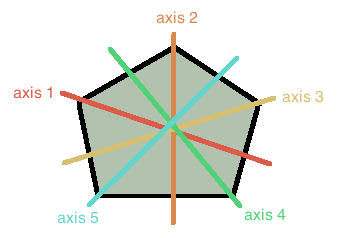
\includegraphics[width=60mm]{Images/dihedral-d5}\]
 Note first that $s$ is not a rotation, so $s\notin \langle r\rangle \leq D_5$. That is $s$ is \textit{another} generator for $D_5$. It remains to determine how $s$ and $r$ interact with \textit{each other}. A quick encounter with reality tells us that $sr=r^{-1}s$, that is, $s$ and $r$ don't quite commute, but there is a rule for swapping their orders. This gives a presentation \begin{equation} 
 	D_5 =\langle s,r \mid s^2=r^5=e, sr=r^{-1}s\rangle
	\end{equation}
\end{example}


\begin{defn}
	The \textbf{dihedral group} of order $n$ is the group $D_n$ given by the following presentation \begin{equation} 
		D_n=\langle s, r \mid s^2=r^n=e, sr=r^{-1}s\rangle \end{equation}
\end{defn}

In general, $D_n$ describes the symmetries of a regular $n$-gon (viewed as a sided shape living in the plane): $r$ is a rotation by $2\pi/n$ and $s$ is a reflection through the origin and a chosen vertex of the $n$-gon. 

\begin{example}[Examples of dihedral groups] For small $n$, we already know the dihedral groups of order $n$ (up to isomorphism, at least). For instance,
\begin{itemize}
	\item $D_1\cong \{e\}$ the trivial group
	\item $D_2\cong \mathbf{Z}_2$
	\item $D_3\cong S_3$, the permutation group on three symbols and the only nonabelian group of order $6$
	\item To describe the groups $D_n$ for $n\geq 4$ requires semi-direct products, which we probably wont get to until later
\end{itemize}
\end{example}

Let $n\geq 1$. The group $D_n$ has order $2n$, since any word can be rearranged to be of form either $r^k$ or $sr^k$ for $k\in\{0,1,\dots,n-1\}$. The cyclic subgroup of $D_n$ generated by $r$ has $\langle r\rangle \cong \mathbf{Z}_n$, similarly $\langle s\rangle \cong \mathbf{Z}_2$. 

\subsection{Exercises}
\begin{enumerate}[label=\arabic*.]

	\item Complete the proof of proposition \ref{crt-group-version}
	\item Let $G=\langle a,b \mid ab=ba\rangle$ is $G$ a finite group? What about $H=\langle a,b \mid ab^2=b^3a\rangle$
	\item How many subgroups of $D_{20}$ have order 5?
	\item Write out the subgroup lattices for $\mathbf{Z}_{20}$, $D_{10}$, and $Q_8$
	\item List all finite abelian groups of order $\leq 40$. (Hint: use theorem \ref{FTFG})
	\item True or False: There is a nontrivial subgroup $H\leq \mathbf{Z}$ such that $H$ is finite. 
	\item Does there exist a subgroup $H\leq D_{20}$ of order $4$?
	\item Prove that the group $Q_8$ from \eqref{Q_8} has exactly eight elements
	\item Let $n\geq 3$, prove that $D_n$ is not a cyclic group
	
	\item Let $S$ be a square with vertices $A,B,C$ and $D$ below. Is it true that \textit{any} permutation of the letters $A,B,C,D$ is a symmetry of this square?
	
	\[ 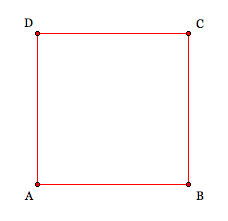
\includegraphics[width=50mm]{Images/square-ex}\]

	\item Let $n,m$ be numbers such that $\gcd(n,m)\neq 1$. Prove that $Z_m \oplus Z_n$ is not cyclic. 
	\item Let $n\geq 1$ and write $D_n$ for the $n$-th dihedral group. Show that $D_n\cong \langle s,r \mid r^n=s^2=(sr)^2=e\rangle$. 
	
	\textit{Challenge} Show that $D_n \cong \langle s,t\mid s^2=t^2=(st)^n=e\rangle$
	
	\item \textit{Challenge} Let $G$ be group generated by the 26 letters of the English alphabet with the relation that words are equivalent if they have the same pronunciation (in English). Show that $G$ is trivial. 
\end{enumerate}

\section{Symmetric groups}

Among the most important finite groups are the symmetric groups (also called permutation groups). In fact, the theory of groups was initially told entirely in terms of symmetric groups and their subgroups.



\begin{defn}
Let $X$ be a finite set. Define $\Sym(X)$ to be the group who elements are bijections $\varphi\colon X\to X$ with the group operation of function composition.
\end{defn}

Let $X$ be a set. In $\Sym(X)$ we denote by $\Id$ the identity function $\Id(x)=x$ for all $x\in X$. Any bijection $\varphi\colon X\to X$ is called a \textit{permutation} of the set $X$. Note that composition of permutations is read \textit{right to left} (consistent with function composition). That is, if $\varphi$ and $\varphi'$ are permutations of $X$, then $(\varphi\varphi')(x)=\varphi(\varphi'(x))$

It's trivial to show that if $X$ and $Y$ have the same number of elements, then $\Sym(X)\cong \Sym(Y)$, therefore the isomorphism type of $\Sym(X)$ really only depends on the number of elements in $X$. For $n\geq 0$ let's set $\underline{0}=\emptyset$ and \begin{equation} \underline{n}=\{1,2,3,\cdots,n\} \qquad \qquad n\geq 1\end{equation}

\begin{defn}[$n$-th symmetric group]
	Let $n\geq 0$, the $n$-th symmetric group is defined to be $S_n=\Sym(\underline{n})$. 
\end{defn}

\begin{prop}
	Let $n\geq 0$. Then $|S_n|=n!$
\end{prop}

\begin{proof}
	This is standard proof by induction. For $n=0,1$ this is trivial. Suppose $n$ given such that we know that $|S_{n-1}|=(n-1)!$. We want to show that $|S_n|=n!$. Let a bijection $\alpha\colon \underline{n}\to \underline{n}$ be given. Suppose that $\alpha(n)=k$. Then $\alpha$ is a bijection of the set $\{1,2,\cdots,n-1\}$ and $\underline{n}\setminus \{k\}$. There are $(n-1)!$ such bijections (by the inductive hypothesis), and $n$ such choices of $k$. So, the total number of bijections $\alpha=n(n-1)!=n!$.
\end{proof}


\begin{remark}
	Since $|S_0|=|S_1|=1$ we must have $S_0\cong S_1\cong \{e\}$ the trivial group. Similarly, $S_2\cong \mathbf{Z}_2$ the only group of order 2. 
	
	For $n\geq 3$, $S_n$ is not abelian. $S_3$ has $3!=6$ elements, so since there are only two groups of order $6$, we must have $S_3\cong D_3$. In fact, this isomorphism can be seen by first labelling the vertices of an equilateral triangle as 1,2,3; then identifying a permutation of $\underline{3}$ with the symmetry from $D_3$ which permutes the vertices in that order. (Note that this does not work for the square (or $n$-gons with $n\geq 4$) since, e.g. no symmetry of the square will swap the vertices $1$ and $2$ keeping $3,4$ fixed.)
	\[ 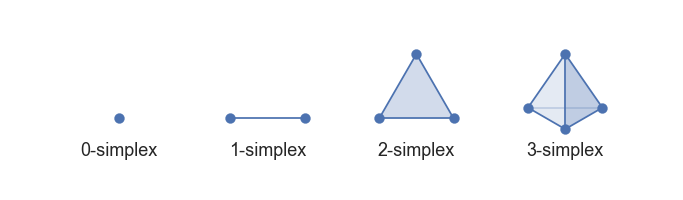
\includegraphics[height=40mm]{Images/simplex-ex}\]
	The natural ``object'' on which the group $S_n$ is the symmetries of is a regular  \href{https://en.wikipedia.org/wiki/Simplex}{$(n-1)$-simplex}. For instance, $S_4$ encodes the symmetries of a regular \href{https://en.wikipedia.org/wiki/Tetrahedron}{tetrahedron} (include those which reverse the orientation of the tetrahedron), which is just a regular $3$-simplex. This is maybe somewhat unsatisfying for $n\geq 5$ since then the geometric objects become $4$+ dimensional which is obviously hard to visualize. 
\end{remark}

\subsection{Cycle decomposition of permutations}

Standard notation for working with permutation groups is to use what is called \textit{cycle notation}. Suppose a permutation from $\alpha\in S_5$ is given by: \[\alpha(1)=2, \quad \alpha(2)=4, \quad \alpha(3)=5, \quad \alpha(4)=3, \quad \alpha(5)=1\]
This is rather clunky, and generally there's not going to be a ``nice'' algebraic formula for a given permutation. We can instead write the information of $\alpha$ as follows $(12435)$. That is, the function is read ``cyclically'' in that \[ 1 \to 2\to 4 \to 3\to 5\to 1\] Since $\alpha$ is a bijection this notation makes sense. In particular, $\alpha$ can just as well be interpreted as a permutation in $S_6$ where the element $6$ is not moved. 

\begin{defn}[Cycle in $S_n$]
	Let $n\geq 0$ and suppose that $\alpha\in S_n$ such that the following holds: There is a number $k$ with $1\leq k\leq n$ and collection of elements $A=\{a_1,\cdots,a_k\}\subset \underline{n}$ such that \[ \alpha(a_1)=a_2, \quad \alpha(a_2)=a_3, \quad \cdots \quad \alpha(a_{k-1})=a_k, \quad \alpha(a_k)=a_1\] and $\alpha(a)=a$ for all $a\notin A$. Then $\alpha$ is called a \textbf{cycle of length $k$} (in $S_n$). In this setup, we write \begin{equation} \alpha=(a_1\, a_2\, a_3\,\cdots \, a_{k-1}\, a_k)\end{equation} for the cycle $\alpha \in S_n$. 

\end{defn}

The word \textit{cycle} here is consistent with the notion of a cyclic group: if $\alpha$ is a cycle of length $k$ then $\langle \alpha\rangle \cong \mathbf{Z}_k\leq S_n$. Let's say that given a cycle $\alpha\in S_n$, and the collection $A$ as outlaid in the above definition, that any $a\in A$ is an \textit{element moved by $\alpha$} (and that if $a\notin A$ then $a$ is \textit{not moved} by $\alpha$). If $\alpha$ is a cycle of length $2$ we call $\alpha$ a \textbf{transposition}.

Let $n\geq 1$ and let $\alpha, \beta$ be cycles in $S_n$. Then, $\alpha$ and $\beta$ are said to be \textbf{disjoint} if they do not move any common elements. Note that while $S_n$ is generally not abelian, the following statement is true.

\begin{prop} \label{disjoint-cycles-commute}
	Let $n\geq 0$. If $\alpha,\beta \in S_n$ are disjoint cycles then $\alpha\beta=\beta\alpha$.
\end{prop} 

\begin{proof}
	Left as an exercise.
\end{proof}

\begin{thm}\label{disjoint-cycles}
	Let $n\geq 0$. Every permutation in $S_n$ is a product of disjoint cycles. Moreover, this decomposition is unique up to rearrangement of factors. 
\end{thm}
\begin{proof}
	This is a nice example of a theorem which is ``evident'' but a bit annoying to write a proof of. Here's the idea. We'll use (complete) induction on $n$. For $n=0,1$ and $2$ this is obvious. 
	
	So let $n$ be given so that for all $k<n$ the claim holds. Let $\alpha\in S_n$. Then $\alpha$ is a bijection of the set $\underline{n}=\{1,2,\dots, n\}$. Consider the set $X=\{1,\alpha(1), \alpha(\alpha(1)), \alpha^3(1),\cdots\}$. Then $X\subset \underline{n}$. If $X=\underline{n}$ we're done, as then $\alpha$ is a cycle of length $n$. If not then we can consider the set $\underline{n}\setminus X$ which must be have a bijection with some set $\underline{k}$ for $1\leq k < n$. So, by induction $\alpha$ restricted to the set $\underline{n}\setminus X$ has a decomposition into disjoint cycles. By construction, these cycles are disjoint from the cycle $(1 \, \alpha(1) \, \alpha^2(1) \cdots)$. So the claim holds. 
	
		Uniqueness I leave to you as an exercise. 
\end{proof}

The decomposition of a permutation $\alpha$ into disjoint cycles is called its \textbf{cycle decomposition}. 
\begin{corollary} \label{trans-generate-Sn}
	Let $n\geq 2$. Every permutation in $S_n$ can be written as a product of transpositions.
\end{corollary}
\begin{proof}
	From theorem \ref{disjoint-cycles} it's enough to show that any cycle can be written as a product of transpositions. Let $2\leq k\leq n$ and $\alpha \in S_n$ be given of the form $\alpha=(a_1\, a_2\, a_3\,\cdots \, a_{k-1}\, a_k)$ for some elements $a_1,\dots,a_k\subset \underline{n}$. Then, by Ex. \ref{permutation-ex} we can write each $\alpha$ a product of transpositions; e.g. as\[\alpha= (a_{1} \, a_2)(a_2\, a_3) \cdots (a_{k-2} \, a_{k-1} )(a_{k-1} \, a_k)\]This completes the proof.
\end{proof} 
\subsection{Conjugacy classes and cycle decomposition}

If $G$ is a group and $g,h\in G$ we call the term $ghg^{-1}$ the conjugate of $h$ by $g$. The first observation is the following:

\begin{prop}
	Let $G$ be a group. Define an relation $\sim$ on $G$ by $h\sim h'$ if there is $g\in G$ with $ghg^{-1}=h'$. Then $\sim$ is an equivalence relation.
\end{prop}

Any set of the associated partition $G/\sim$ is called a \textbf{conjugacy class} of $G$. If $h,h'\in G$ such that there is a $g\in G$ such that $ghg^{-1}=h'$ we say that $h$ and $h'$ are \textbf{conjugate} (by $g$). 

\begin{example}
	We've seen an example of this before\footnote{I believe I showed this in class way back in the first or second week}. In the group $\GL_2(\mathbf{R})$ (with matrix multiplication), matrices $A$ and $B$ are conjugate if and only if there is $P\in \GL_2(\mathbf{R})$ with $PAP^{-1}=B$. In this case, $A$ and $B$ must have the same eigenvalues. In fact, matrices $A,B\in \GL_2(\mathbf{R})$ are conjugate if and only if they have the same eigenvalues. 

\end{example}


\begin{prop} Let $n\geq 0$ and $\alpha,\beta\in S_n$. Suppose that $\alpha$ is a cycle of length $k$ given by $\alpha=(a_1 \, a_2\, \cdots \, a_k)$. Then \[\beta\alpha\beta^{-1}=(\beta(a_1) \, \beta(a_2)\, \cdots \, \beta(a_k))\]

\end{prop}
In particular, any conjugate of a cycle of length $k$ in $S_n$ is another cycle of length $k$. 


\begin{defn}
Let $n\geq 0$ and $\alpha\in S_n$. Let $k\geq 1$ and $n_1,n_2,\dots,n_k\geq 1$ such that $n_1+n_2+\cdots+n_k=n$. We say that $\alpha$ is a \textbf{cycle of type $(n_1,n_2,\cdots,n_k)$} if $\alpha$ has a decomposition into disjoint cycles $\alpha=\alpha_1\alpha_2\cdots\alpha_k$ such that $\alpha_i$ is a cycle of length $i$ for $i=1,2,\dots,k$. 
\end{defn}

Note by theorem \ref{disjoint-cycles} that any decomposition of a permutation $\alpha\in S_n$ into cycles must have the same cycle type. 


\begin{thm}
	Let $n\geq 0$. The conjugacy classes of $S_n$ are in one-to-one correspondence with the cycle types of $S_n$. 
\end{thm}

\begin{example}
	In $S_2$ there are two conjugacy classes: $\{\Id\}$ and $\{(12)\}$. These correspond to the two decompositions $2=2$ and $2=1+1$.
	
	In $S_3$ we have conjugacy classes corresponding to the decompositions of $3$ as $3=3, 3=2+1$ and $3=1+1+1$. These correspond to the conjugacy classes \[ \{ (123), (231) \}, \quad \{ (12), (23), (13)\}, \quad \{ \Id\}\]
	
\end{example}



\subsection{Sign of a permutation}

From corollary \ref{trans-generate-Sn} we know that transpositions generate $S_n$. 


\begin{thm} \label{id-is-even}
	Let $n\geq 0$. If $k\geq 1$ and $\alpha_i\in S_n$ is a transposition for $i=1,\cdots,k$ such that $\Id=\alpha_1\alpha_{2}\alpha_3 \cdots \alpha_k$; then $k$ is an even number.
\end{thm}
\begin{proof}
	A warning, this is somewhat of a tricky proof. We use proof by induction. The identity cannot be a transposition, so $k\neq 1$. If $k=2$ then this follows since any transposition is its own inverse. 
	
	So, let $k>2$ such that the claim holds for all integers $\ell$ with $2\leq \ell < k$. Let $\alpha_k=(a\,b)$, there are then four cases to consider for the form of the terms $\alpha_{k-1}\alpha_k$: \[ \text{(i) } (a \, b)(a\, b),  \quad\text{(ii) } (a \, c)(a\, b) , \quad\text{(iii) } (b \, c)(a\, b) , \quad\text{(iv) } (c \, d)(a\, b)\]
	(here, $c,d\in \underline{n}$)
	
	Let's go case by case. In case (i), we have that $(a\, b)(a\, b)=\Id$, so that $\alpha$ can be reduced to a string of $k-2$ transpositions. By induction, $k-2$ must be even, $k=(k-2)+2$ is even as well. 
	
	In cases (ii)--(iv) we can use the following equations (you should verify these)  \begin{equation} (a\,c)(a\,b)=(a\, b)(b\, c)\, \quad (b\,c)(a\, b)=(a\,c)(c\,b), \quad (c\,d)(a\,b)=(a\,b)(c\,d) \end{equation} to replace $\alpha_{k-1}\alpha_k$ by an equivalent pair of transpositions with $a$ not appearing in $\alpha_k$. If $\alpha_{k-1}=\alpha_{k-2}$ then we're done by induction: cancel these terms and learn by induction that $k-2$ must be even. If not, we can run the same operation again replacing $\alpha_{k-2}\alpha_{k-1}$ by an equivalent string with $a$ not appearing in the term $\alpha_{k-1}$. 
	
	Now let's look at the product $\alpha_1\alpha_2\cdots\alpha_{k-2}$. If this is the identity then we're done, since by the inductive hypothesis we must have $k-2$ even, and therefore $k$ even as well. If not, then we can continue this game: replace $\alpha_{k-3}\alpha_{k-2}$ by a pair of equivalent transpositions with $a$ moved by $\alpha_{k-3}$ only, then $\alpha_{k-4}\alpha_{k-3}$, etc. The claim is that at some point, this pairwise exchange of transpositions must produce the same transposition next to itself. This then cancels out, leaving $\Id$ written as a product of $k-2$ transpositions, and the theorem follows. 
	
	Suppose that this never happens. Then we can exchange transpositions all the way back to $\alpha_1\alpha_2$ such that $\alpha_1$ moves $a$ and no $\alpha_k$ for $k\geq 2$ does. This is a problem, because by assumption we must still have $\Id=\alpha_1\alpha_2\cdots\alpha_k$; but if only $\alpha_1$ moves then $\Id(a)\neq a$ as would be required. This completes the proof.\end{proof} 

\begin{corollary} \label{sign-is-well-def}
	Let $n\geq 0$ and $\alpha\in S_n$ some permutation. If $\alpha$ is represented as an even number of transpositions, then any other representation of $\alpha$ by transpositions must also contain an even number of factors. Similarly, if $\alpha$ is represented as an odd number of transpositions, then any other representation of $\alpha$ by transpositions must contain an odd number of factors. 
\end{corollary}

\begin{proof}
	 Suppose that we had two representations of $\alpha$ by transpositions, i.e., that\[\alpha=\tau_1\tau_2\tau_3\cdots\tau_n=\sigma_1\sigma_2\sigma_3\cdots\sigma_m\] where $\tau_i$ and $\sigma_j$ are transpositions for $i=1,\dots,n$ and $j=1,\dots,m$. The first claim is that \[ \alpha^{-1}=\tau_n \tau_{n-1}\cdots \tau_3\tau_2\tau_1\] Indeed, any transposition is its own inverse, so that \[\tau_1\tau_2\cdots\tau_{n-1}\tau_n\tau_n\tau_{n-1}\cdots\tau_2\tau_1=\tau_1\tau_2\cdots\tau_{n-1}\tau_{n-1}\cdots \tau_2\tau_1=\cdots=\tau_2\tau_1\tau_1\tau_2=\tau_1\tau_1=\Id.\] Then we cxan write \[ \Id=\alpha \alpha^{-1}=\sigma_1\sigma_2\sigma_3\cdots\sigma_m\tau_n \tau_{n-1}\cdots \tau_3\tau_2\tau_1\] But, by theorem \ref{id-is-even} we must have $n+m$ be an even number. This means that either $n$ and $m$ are both even or $n$ and $m$ are both odd. Thus the claim is proved. 
\end{proof}

\begin{defn}[Sign of permutation]
Let $n\geq 0$ and $\alpha\in S_n$. Let $k$ be the number of transpositions in some representation of $\alpha$ by transpositions. If $k$ is even, $\alpha$ is called an \textbf{even} permutation; if $k$ is odd, $\alpha$ is called an \textbf{odd} permutation.
\end{defn}

It's worth pointing out that corollary \ref{sign-is-well-def} tells us that this definition is indeed well-defined. The number of individual transpositions in some representation of a permutation $\alpha\in S_n$ is not necessarily unique, but the \textit{parity} (i.e., even or oddness) of that number is. You can think of this a function \begin{equation} \operatorname{sgn}\colon S_n \to \mathbf{Z}_2\end{equation} such that $\operatorname{sgn}( \text{even permutations})=0$ and $\operatorname{sgn}(\text{odd permutations})=1$. In fact, $\operatorname{sgn}$ is a homomorphism $S_n\to \mathbf{Z}_2$ (see Ex. \ref{sgn-hom}). We'll dig deeper into general homomorphisms (i.e., not just isomorphisms) in the next section. 



\subsection{The alternating group}

Let $n\geq 0$ and define $A_n\subset S_n$ to be \begin{equation} A_n=\{ \alpha\in S_n : \text{$\alpha$ has a representation as an even number of transpositions}\}\end{equation}
The following proposition tells us that $A_n$ is indeed a subgroup of $S_n$. We call $A_n$ the \textbf{alternating group} (on $n$ symbols). 
\begin{prop} $A_n$ is a subgroup of $S_n$
\end{prop}
\begin{proof} $\Id=\tau^{2}$ for any transposition $\tau$, so $\Id\in A_n$. If $\alpha,\beta \in A_n$, then $\alpha$ and $\beta$ both have presentations as an even number of transpositions. Since the sum of even numbers is even, $\alpha\beta\in A_n$ then. Similarly, if $\alpha=\tau_1\tau_2\cdots\tau_k$ is decomposed into transpositions $\tau_i$, then $\alpha^{-1}=\tau_k\tau_{k-1}\cdots\tau_1$, which has the same number of transpositions. So if $\alpha\in A_n$ then $\alpha^{-1}\in A_n$ as well. 
\end{proof}

\begin{prop} \label{order-of-An}
	Let $n\geq 2$, then $|A_n|=n!/2$.
\end{prop}

Either a permutation is even or odd, so it's half the total permutations (that's a joke, but only sort of).  Let $A_n\subset S_n$ be the even permutations and $O_n\subset S_n$ be the odd permutations. Note that $A_n$ and $O_n$ are disjoint, so if we show that there is a bijection $A_n\to O_n$ we're done. Fix any transposition $\tau\in S_n$ and define $\varphi\colon A_n\to O_n$ by $\varphi(\alpha)=\tau\alpha$. Note that if $\alpha\in A_n$ then $\tau\alpha$ has one more transposition, so is odd, and therefore this function is well defined. 

Let's show that $\varphi$ is a bijection. $\varphi$ is injective as, if $\tau\alpha=\tau\beta$ for some permutations $\alpha,\beta\in A_n$, then $\alpha=\tau\tau\alpha=\tau\tau\beta=\beta$. Similarly if $\beta\in O_n$ then $\tau\beta\in A_n$ and $\varphi(\tau\beta)=\tau\tau\beta=\beta$, so $\varphi$ is surjective as well. Thus $|A_n|=|O_n|$ and therefore since $|A_n|+|O_n|=|S_n|=n!$ we must have $|A_n|=n!/2$. 

\subsection{The alternating group in action}

\begin{example}
	It's straightforward to check that $A_1=A_2=\{\Id\}$. A calculation reveals that $A_3=\{\Id, (123), (132)\}\cong \mathbf{Z}_3$. $A_3$ can be interpreted as the orientation-preserving symmetries of the regular $2$-simplex; that is, the subgroup $\langle r\rangle \leq D_3$. 
	
	For $n\geq 4$, $A_4$ is not abelian. It's possible to enumerate the elements of $A_4$: \[A_4=\{ \Id, (12)(34), (13)(24), (14)(23), (123), (132), (124), (142), (134), (143), (234), (243) \}\]
	This is a non-abelian group corresponding to the orientation-preserving\footnote{That is, if you have an honest tetrahedron (a four-sided die, say) in the $3$d space in which we live, the symmetries of that tetrahedron. Some people/books/authority figures will say this $A_4$ is indeed the group of symmetries of the tetrahedron but this inconsistent with $D_3$ being the group of symmetries of the equilateral triangle. ``Symmetries'' in this context is not exactly clear enough: only those from the alternating group preserve the orientation of the space these shapes are immersed into.} symmetries of a regular tetrahedron. It's one of the five non-isomorphic groups of order $12$; we know three of the others: $\mathbf{Z}_{12}, \mathbf{Z}_6\oplus \mathbf{Z}_2$ and $D_6$. The last has the presentation $\langle a, b, c\mid a^3=b^2=c^2=abc=e\rangle$\footnote{Groupprops tells me this is called the \href{https://groupprops.subwiki.org/wiki/Dicyclic_group:Dic12}{\textit{Dicyclic group}}, so I suppose I must believe them}. It's not supposed to be obvious that these are all the groups of order 12.  \end{example}

	\begin{example}[$A_n$ and roots of polynomials] You may know of the following theorem: 
	
	\begin{quote}\textit{Let $p$ be a polynomial with real coefficients of degree $n$. There is an explicit formula for the roots (i.e., $x$ such that $p(x)=0$) of $p$ using radicals if and only if $n=1,2,3,4$}. \end{quote}
	
	For instance, if $n=2$ there is the good old quadratic formula. For $n=3,4$ there are corresponding cubic and quartic formulas which become increasingly complicated. There is, however, no general formula for $5$-th and larger degree polynomials using only roots. This has to do with the structure of the groups $A_n$, in particular that $A_n$ is not \textit{solvable}\footnote{Being \href{https://en.wikipedia.org/wiki/Solvable_group}{solvable} is weaker than being abelian, but still somewhat similar. We probably won't get to talk about solvability of groups} for $n\geq 5$. It's a lot more involved group theory and Galois theory to show this, but an interesting and nontrivial connection to what we're learning. \end{example}



\begin{example}[Symmetry groups of the Platonic solids] \label{platonic-solids-ex}
A neat application of symmetric and alternating groups comes from the groups of symmetries of the five \href{https://en.wikipedia.org/wiki/Platonic_solid}{Platonic solids}. Recall that a platonic solid is a polyhedron in $\mathbf{R}^3$ all of whose faces are the same. There are only five such polyhedra: The cube, the tetrahedron, the octahedron, the icosahedron, and the dodecahedron. 

A \textbf{rotational symmetry} means \textit{orientation-preserving symmetry}\footnote{For instance, the reflection $s\in D_n$ are not rotational symmetries of the $n$-gon. Recall that a rotation of the plane is given by the matrix \[\begin{pmatrix} \cos(\theta) & - \sin(\theta) \\ \sin(\theta) & \cos(\theta) \end{pmatrix}\] for some $\theta\in\mathbf{R}$. If we view the $n$-gon as living inside $\mathbf{R}^2$, no such rotation matrix will take the $n$-gon to its reflection (such a matrix would have to have a negative determinant). It's maybe a bit subtle to really define what a rotation is: one way is to say that a rotation in $\mathbf{R}^n$ is an element of the special orthogonal group $\operatorname{SO}(\mathbf{n})$ of orthogonal $n\times n$ matrices with determinant $1$. This a good example of what's called a Lie group, I'd like to talk about these more later in the term.}, which is again to say, some symmetry you could realize as an honest symmetry of the shape $X$ in $\mathbf{R}^3$. We have the following
\[\begin{tabular}{l | l| l | c}
Solid &  Shape of faces & Number of faces &Rotational symmetry group \\ \hline
Tetrahedron & Triangle & 4 & $A_4$ \\
Cube & Square & 6 & $S_4$ \\
Octahedron & Triangle & 8 & $S_4$ \\
Dodecahedron & Pentagon & 12 & $A_5$ \\
Icosahedron & Triangle & 20 & $A_5$\\
\end{tabular}\]

What's more is that, together with the cyclic and dihedral groups, the groups appearing in the above table are the \textit{only} finite groups that can be realized as the rotational symmetry of some polyhedron in $\mathbf{R}^3$. 
\end{example}

\subsection{Subgroups of $S_n$}

In general, any finite group can be embedded\footnote{This has a precise definition, i.e., that a group $H$ embeds into $G$ if there is an injective homomorphism $H\to G$.} into a symmetric group. As mentioned before, ``groups'' as a concept were initially thought of inasmuchas their embeddings into $S_n$ for some $n$. Cayley's theorem, as follows, solidifies this interpretation. We'll talk more about some of the subtletites of this argument when we discuss group actions in depth.


\begin{thm}[Cayley's theorem] 
Let $n\geq 1$ and $G$ be any finite group of order $n$. Then $G\leq S_n$. 
\end{thm}

\begin{proof}
	Let $n\geq 1$ and suppose that $G$ is any finite group of order $n$. Let's define $X_G$ to be the set with the same elements as $G$, and define  $\widetilde{G}$ to be the set of functions $\varphi_g\colon X_G\to X_G$ given by $\varphi_g(x)=gx$ for $g\in G$. Any such function $\varphi_g$ is a bijection (you should prove this), and  so  $\widetilde{G} \subset \Sym(X_G)$. The first claim is that  $\widetilde{G}$ is indeed a subgroup of $\Sym(X_G)$, the second is that $G\cong  \widetilde{G}$. Let $n=|G|$, then since $X_G$ is a set with $n$ elements, $\Sym(X_G)\cong S_n$, which proves the theorem.
\end{proof}

\subsection{Exercises}
\begin{enumerate}[label=\arabic*.]
	\item Let $\alpha=(12), \beta=(23)$ and $\gamma=(34)$. Construct a presentation of the symmetric group $S_4$ with generators $\alpha,\beta$ and $\gamma$. 
	\item Let $\alpha=(a_1\,a_2\,\cdots\,a_k)\in S_n$. Prove that $\alpha=(a_2 \, a_3\, \cdots\, a_k \, a_1)$ and $\alpha^{-1}=(a_k\, a_{k-1}\, \cdots\, a_1)$
	\item Construct a generating set for $A_4$ and write a presentation based on your set of generators. 
	\item Let $H=\{\alpha\in S_5 : \alpha(1)=4\}$. Is $H\leq S_5$?
	\item Prove proposition \ref{disjoint-cycles-commute}.
	\item Let $\alpha,\beta\in S_n$ such that  $\alpha$ is a cycle of length $k$ of the form $\alpha=(a_1\,a_2\,\cdots \, a_k)$. Prove that  \[\beta\alpha\beta^{-1}=(\beta(a_1) \, \beta(a_2)\, \cdots \, \beta(a_k))\]
	\item Recall that $Z(G)=\{ g\in G : gh=hg \text{ for all $h\in G$}\}$. Prove that $Z(S_n)=\{\Id\}$ for all $n\geq 3$.
	\item Determine (i) the cycle decomposition of, (ii) the order of each of the following permutations \begin{enumerate}
		\item $(12)(357)$
		\item $(12)(237)$
		\item $(345)(245)$
		\item $(1235)(24567)$
	\end{enumerate}
	\item Let $\alpha$ be a $6$-cycle and $\beta$ be a $5$-cycle. Determine if $\alpha^4\beta^4\alpha^{-1}\beta^2$ is even or odd.
	\item Describe all conjugacy classes (i.e., cycle types) in $S_7$ and $A_7$. 
	\item Show that $A_{10}$ contains an element of order $5$. 
	\item Prove that $A_3$ is the group of orientation-preserving symmetries of a regular $3$-gon\footnote{You may know this shape by the name \textit{equilateral triangle} (but it will also be the regular 3-gon to me).} Harder: prove that $A_4$ is the group of orientation preserving symmetries of a regular tetrahedron. \
	\item \label{permutation-ex} Let $n\geq 0$ and write $\alpha=(a_1\,a_2\,a_3\,\cdots,a_k)$ for some cycle in $S_n$. Prove that $\alpha$ can be decomposed into transpositions in the two following ways
	\[ \alpha=(a_1\,a_k)(a_1 \, a_{k-1})\cdots (a_1\,a_3)(a_1\,a_2)=(a_1\,a_2)(a_2\,a_3)\cdots(a_{k-2}\,a_{k-1})(a_{k-1}\,a_k)\]
	\item Let $D_n$ be the $n$-th dihedral group. Prove that $D_n\leq S_n$ for all $n\geq 1$. 
	\item \label{sgn-hom}Prove that $\operatorname{sgn}\colon S_n\to\mathbf{Z}_2$ is a homomorphism. 
	\item Let $\alpha,\beta \in S_n$. Prove that their \textit{commutator} $\alpha\beta\alpha^{-1}\beta^{-1}$ is always an element of $A_n$.
	\item True or False: For any $n\geq 3$, there is a presentation of $S_n$ with exactly two generators. 
	\item True or False: If $\alpha\in S_n$ is a cycle, then $\alpha^k$ is a cycle for all $k\geq 1$.

	\item \textit{Challenge}. Prove that the group of rotational symmetries of a regular cube in $\mathbf{R}^3$ is isomorphic to $S_4$. Use that the octahedron and cube are \href{https://en.wikipedia.org/wiki/Dual_polyhedron}{\textit{dual}} (as polyhedra) to show that the group of rotational symmetries of a regular octahedron is also $S_4$. 
	
	\textit{Challeng-ier}. Use the same type of duality argument to prove that the regular icosahedron and dodecahedron both have rotational symmetry group isomorphic to $A_5$.
	\item \textit{Challenge}. Let $n\geq 1$. Describe the set $K_n$ of all integers $k$ for which $S_n$ has a subgroup of order $k$.
	\item ($A_n$ is generated by $3$-cycles). Let $n\geq 3$. Prove that $(a\,b)(c\,d)=(a\,c\,b)(a\,c\,d)$ and $(a\,b)(a\,c)=(a\,c\,b)$ for any $a,b,c,d\in \underline{n}$. Use this to prove that the collection of cycles of length $3$ generate $A_n$. 
\end{enumerate}

\section{Normal subgroups and group quotients}

So far we've seen many examples of group, and some examples of how to construct new groups from old. One crucial operation is missing: Quotients. The first observation is that not all subgroups ``permit" quotienting. In order to create a quotient of a group by a subgroup, we need to first describe the language of cosets.

\subsection{Cosets}

Let $G$ be a group and $H\leq G$ some subgroup of $G$. Let $g\in G$. We write $gH$ and $Hg$ for the sets \begin{equation} gH=\{gh : h\in H\} \qquad \qquad Hg=\{hg: h\in H\} \end{equation}
In words, a set of the form $gH$ is called a \textbf{left coset}\footnote{Note that $g$ acts on the \textit{left} here} of $H$ by $g$ (in $G$), and $Hg$ is called a \textbf{right coset} of $H$ by $g$ (in $G$).  Note that in general these sets are not equal, since groups are not assumed to be commutative. Note that cosets $gH$ and $g'H$ may have $gH=g'H$ without group elements $g$ and $g'$ being equal. 

\begin{prop}
	Let $G$ be a group and $H\leq G$. Then $g\sim h$ if and only if $gH=hH$ is an equivalence relation on $G$. Similarly, $g\sim h$ iff $Hg=Hh$ is also an equivalence relation on $G$.
\end{prop}

I believe we proved the above proposition (or something equivalent to it) in lecture. Regardless, I leave it to you as an exercise. The key here is that cosets (either left or right) form a partition of the original group $G$. 

\begin{example} Recall that any subgroup $H\leq \mathbf{Z}$ is of the form $H=n\mathbf{Z}=\{nk: k\in \mathbf{Z}\}$ for some $n\in \mathbf{Z}$. Such a subgroup has cosets given by the equivalence classes $[0], [1], \cdots, [n-1]$ where again \[ [k]=\{k+n\ell : \ell\in\mathbf{Z}\}=k+n\mathbf{Z}\]
In this case, cosets $k+n\mathbf{Z}$ and $n\mathbf{Z}+k$ are equal, since addition of integers is commutative. 
\end{example}

\begin{remark}
	 In general, if $H\leq G$ and $g\in G$ such that $gH\neq eH$, then $gH$ \textbf{will not} be a subgroup of $G$. An upshot is that a lot of the intuition from linear algebra carries over. A subgroup $H\leq G$ is analogous to a \textit{subspace} $U\subset V$ of some vector space $V$ (i.e., $V=\mathbf{R}^n$). Recall that all subspaces must contain the origin, in the same way that all subgroups must contain the identity. Cosets of $U$ in $V$ are the translations of $U$ by some nonzero vector: i.e., $v+U$ for some $v\in V$. They aren't quite subspaces\footnote{Sometimes you'll see the adjective \textit{affine} used here}, but \textit{shifts} of subspaces.
\end{remark}

\subsection{Normal subgroups}

For certain types of subsets of $G$, it is possible to define a group structure on the set of cosets. These subsets are called normal subgroups as we discuss below.

\begin{defn}[Normal subgroup]
	Let $G$ be a group and $N\leq G$ a subgroup of $G$. We say that $N$ is a \textbf{normal} subgroup of $G$ if for any $g\in G$ we have \begin{equation} gNg^{-1}=\{ghg^{-1} : h\in N\}=N.\end{equation}
\end{defn} 
Notation-wise, we write \begin{equation} N\nrml G\end{equation} to denote that $N\leq G$ is a normal subgroup of $G$. This operation of multiplying by $g$ on the left and $g^{-1}$ on the right is called \textbf{conjugation}---we will see this appear more in the term. An equivalent statement to $N$ being normal is that all \textit{conjugates} of $N$ are the same. 

\begin{prop} Let $G$ be a group. The follow statements are equivalent
\begin{enumerate}[label=(\roman*)]
	\item $N$ is a normal subgroup of $G$
	\item $gN=Ng$ for all $g\in G$ (i.e., left and right cosets of $N$ are the same)
	\item $gNg^{-1}\subset N$ for all $g\in G$
\end{enumerate}
\end{prop}

\begin{proof} Note first that, for any $g\in G$, $gNg^{-1} =N$ if and only if  $gN=gNg^{-1}g=Ng$. This shows (i) is equivalent to (ii). Clearly (i) implies (iii), so it's enough to show that (iii) implies (i). Suppose that $gNg^{-1}\subset N$ for all $g\in G$. Then \[ N = g^{-1} gNg^{-1} (g^{-1})^{-1}\subset g^{-1} N g\] for all $g\in G$. In particular, rewriting $h=g^{-1}$, $N\subset hNh^{-1}$ for all $h\in G$. \end{proof} 

The following proposition is basically trivial, but still very useful to have for reference. I leave it to you to show why this is trivial.
\begin{prop} If $G$ is abelian, and $N\leq G$ then $N\nrml G$.
\end{prop}



\subsection{Quotient groups} 
Given any subgroup $H\leq G$ we write $G/H$ for the set of (left) cosets of $H$ in $G$ (that is, the associated set of equivalence classes given by the partition by left cosets). Note that this is generally different from the partition of $G$ by \textit{right} cosets, you may see people write $H\backslash G$ for this. The distinction is important, but let's no worry about it for now.


\begin{thm}[Quotient group]
	Let $G$ be a group and $N\nrml G$ a normal subgroup. Then $G/N$ inherits a group structure from $G$. 
\end{thm}


\begin{proof}
Let $gN,gH\in G/H$. The evident group operation is given by \[ (gN)(hN)=(gh)N\] Note that this is well-defined since $N$ is normal in $G$; i.e., $(gN)(hN)=g(Nh)N=g(hN)N=ghN$. Moreover, this product does not depend on choice of representative for each coset. Meaning, if $gN=g'N, hN=h'N$ then $g'=gn$ and $h'=hm$ for some elements $n,m\in N$. Then \[(g'N)(h'N)=(g'h')N=(gnhm)N=ghn'mN=ghN\] (note here that $nh=hn'$ for some $n'\in N$ since the right coset and left coset by $h$ agree.) The identity in $G/N$ is given by the subgroup $N=eN$. If $gN\in G/N$ then $(gN)^{-1}=g^{-1}N$. 
%	We must show that the binary operation \eqref{normal-operation} defines a group structure on $G/N$. First of all, this means showing that $[g][h]$ and $[gh]$ are actually the same coset of $N$. Let $g,h\in G$. Then \begin{equation} (gN)(hN)=g(Nh)N=ghNN=(gh)N\end{equation}. It is then straightforward to show that (i) if $e\in G$ is the identity, $[e]$ is the identity in $G/N$, (ii) for any $g\in G$, [g]^{-1}=[g^{-1}]
\end{proof}

The resulting group $G/N$ is called the \textbf{quotient of $G$ by $N$}. Some examples below:

\begin{example}[Quotients of cyclic groups]
	 Let $n\geq1$, then $n\mathbf{Z}=\{nk:k\in \mathbf{Z}\}$ is a normal subgroup of $\mathbf{Z}$. The quotient $\mathbf{Z}/n\mathbf{Z}\cong \mathbf{Z}_n$.
	As another example, let $n\geq 1$ and $k\mid n$. Then $\langle n/k\rangle\nrml \mathbf{Z}_n$. In particular, $\mathbf{Z}/\langle n/k\rangle \cong \mathbf{Z}_k$.
\end{example}

\begin{example}[Normal subgroups of $D_n$] \label{ex-Dn-normal} Let $n\geq 1$. The dihedral group $D_n=\langle r, s \mid r^n=s^2=e, sr=r^{-1}s\rangle$ has the subgroup $N=\langle r\rangle \cong \mathbf{Z}_n$. The claim is that subgroup is normal in $G$. We'll show that $gNg^{-1}\subset N$ for all $g\in G$. It suffices to show this for the generators $s,r$ of $D_n$. That $rNr^{-1}\subset N$ is trivial. To show that $sNs^{-1}\subset N$ we observe that an element in $sNs^{-1}$ is one of the from $sr^ks$, which by the group relations can be rewritten $sr^ks=r^{-k}ss=r^{-k}\in N$. 
	
	The associated quotient group $D_n/\langle r\rangle= \{eN, sN\}\cong \mathbf{Z}_2$. Note that this quotient group is ``crushes'' the rotational aspect of $D_n$, leaving only the reflections. In terms of the presentation, we're simply adding in an additional relations which say any $g\in N$ is equal to $e$. 
\end{example}


\begin{defn}[Index of $H$ in $G$]
Let $G$ be a group and $H\leq G$ any subgroup. The \textbf{index of $H$ in $G$} is the positive integer $n$ such that the partition of $G$ by cosets of $H$ has exactly $n$ elements. 
\end{defn}
We write $[G:H]$ for the index of $H$ in $G$. If $G/H$ has infinitely many elements we write $[G:H]=\infty$\footnote{Technically, you should worry about the cardinality of infinity here, but we'll let this slide}. Note that if $G,H$ are finite groups then $[G:H]$ is always finite. If $G$ is an infinite group there could still be (infinite) subgroups $H$ such that $[G:H]$ is finite. 

In example \ref{ex-Dn-normal} we found that $\langle r\rangle \leq D_n$ is a subgroup of index $2$. Similarly, $A_n\leq S_n$ is a subgroup of index 2. In general, any subgroup of index $2$ is normal (see problem \ref{subgroup-of-index-2}). 


%\begin{example}[Group presentations are quotients of the free group]Let's work with a concrete example first. Let $DC_3=\langle a,b,c \mid a^3=b^2=c^2=abc=e\rangle$. We claim that $DC_3$ is (isomorphic to) a quotient of the free group $\langle a,b,c\rangle$. Let $N$ be the collection of all ``words'' made from the symbols $a^3, b^2, c^2$ or $abc$ (that is, all of the things we wish to set equal to $e$). \end{example}

\subsection{Kernel and image of a homomorphism}

\begin{defn}
	Let $G,H$ be groups and $\varphi\colon G\to H$ a homomorphism. Define the \textbf{kernel}, $\ker{\varphi}$, and \textbf{image}, $\img{\varphi}$, of $\varphi$ by \begin{equation} \ker{\varphi}=\{ g\in G : \varphi(g)=e_H\} \qquad \qquad \img{\varphi}=\{\varphi(g): g\in G\} \end{equation}
	\end{defn}

\begin{prop}\label{ker-is-normal}
Let $G,H$ be groups and $\varphi\colon G\to H$ a homomorphism. Then $\ker{\varphi}\leq G$ and $\img{\varphi}\leq H$.  Moreover, $\ker{\varphi}$ is a normal subgroup of $G$.
\end{prop}

\begin{proof}
	Let $\varphi\colon G\to H$ be given and write $K=\ker \varphi$.  Note that $\varphi(e_G)=e_H$ so that $e_G\in K$. Similarly, if $g,h\in \ker\varphi$ then $\varphi(gh^{-1})=\varphi(g)\varphi(h)^{-1}=e_He_H^{-1}=e_H$. So that $K\leq G$. To show that $K$ is normal, let $g\in G$. Note that $gK=\{gh : \varphi(h)=e_H\}$. So for any $h\in K$ we claim that $gh=h'g$ for some other $h'\in K$. Indeed, set $h'=ghg^{-1}$, then \[\varphi(h')=\varphi(g)\varphi(h)\varphi(g^{-1})=\varphi(g)e_H\varphi(g)^{-1}=e_H\] so that $h'\in K$. Thus $gK=K g$, and so $K$ is normal. That $\img\varphi\leq H$ we leave as an exercise. 
\end{proof}

Generally whenever you have a function $f\colon A\to B$ between sets with algebraic structure, the ``stuff'' in $A$ that gets sent to the identity in $B$ will always be a ``nice'' subset of $A$. 

For instance, you may recall the nullspace of a matrix: Any matrix represents a linear transformation $T\colon V\to U$ for some vector spaces $V,U$ (for instance, $\mathbf{R}^n$). Vector spaces generally have more structure than just a group\footnote{A vector space is what is called a \textit{module} over a \textit{field}. Fields are algebraic structures where you can add, subtract, multiply and divide, like $\mathbf{R}$ or $\mathbf{C}$. \textit{Module} means that in addition to the (abelian) group structure (addition of vectors) you can also multiply by scalars from the field.}, but do always have an underlying (abelian) group whose operation is sum of vectors. The nullspace of $T$ is a linear subspace of $V$ of vectors which get sent to the zero vector in $U$. This is simply the kernel of the linear transformation $T$. 

\begin{prop}
	Let $\varphi\colon G\to H$ be a group homomorphism. Then $\varphi$ is injective if and only if $\ker\varphi=\{e\}$.
\end{prop}

The idea of this proof is that since groups have inverses, any property can be ``shifted'' to the identity. Essentially, one-to-one-ness at the identity is enough to show one-to-one-ness overall. 

\begin{proof}
Suppose that $\varphi$ is injective and write $e\in G$ and $e'\in H$ for th respective group identities. Since $\varphi(e)=e'$ must be true of a homomorphism, then $\ker\varphi=\{e\}$ since $\varphi$ is injective. 
	Similarly, suppose that $\ker\varphi=\{e\}$ and that $g,h\in G$ such that $\varphi(g)=\varphi(h)$. Then $\varphi(gh^{-1})=e'$ so that $gh^{-1}\in \ker\varphi$. But then $gh^{-1}=e$ so that $g=h$. Thus $\varphi$ is injective.
\end{proof}

\subsection{The isomorphism theorems}

The following are some general statements about the structure of groups, mostly regarding quotients, which on the whole are called ``The isomorphism theorems''. However, the isomorphism theorems do not form an ordered set, or even a set with a well-defined cardinality.  As far as labeling which theorem is which, it's the wild west out there. It seems to be a long standing tradition in the world of Algebra textbook authors to use whatever bespoke enumeration is at their particular whim. I'm presenting them here with the enumeration roughly by which I learned them, which comes from the book \textit{Abstract Algebra} by Dummit and Foote. But just be warned, saying ``the $n$-th isomorphism theorem'' is about a precise as saying ``Euler's theorem''. 

\begin{thm}[First isomorphism theorem] \label{first-iso}
	Let $G,H$ be groups and $\varphi\colon G\to H$ a homomorphism. Then $G/\ker{\varphi}\cong \img{\varphi}$
\end{thm}

\begin{proof}
	Write $K=\ker\varphi$ and $I=\img\varphi$. From proposition \ref{ker-is-normal} we know that $K\nrml G$, so the quotient $G/K$ is well-defined. Let's $f\colon G/K \to I$ by $f(gK)=\varphi(g)$. The claim is that $f$ is an isomorphism. 
	
	First, let's show that $f$ is well-defined, this means that if $gK=hK$ represent the same coset in $G/K$ then $f(gK)=f(hK)$. Note that if $gK=hK$ then $h=gk$ (note $\varphi(k)=e$) for some $k\in K$. Therefore, \[f(gK)=\varphi(g)=\varphi(g)e=\varphi(g)\varphi(k)=\varphi(gk)=\varphi(h)=f(hK)\]

	Second, we'll show that $f$ is actually a homomorphism. This follows from the observation that \[ f(gKhK)=f(ghK)=\varphi(gh)=\varphi(g)\varphi(h)=f(gK)f(hK).\]
	
	That $f$ is onto is essentially trivial. If $h\in I$ then $h=\varphi(g)$ for $g\in G$ so $f(gK)=h$. That $f$ is injective follows from the observation that if $f(gK)=f(hK)$ then $\varphi(g)=\varphi(h)$ so that $\varphi(g^{1}h)=e$ and therefore $g^{-1}h\in K$. But $g^{-1}h\in K$ if and only if $gK=hK$. This completes the proof. 
\end{proof}

\begin{remark}
This is a great opportunity to introduce what is called a \textbf{commutative diagram}. That is, a direct graph, where arrows between nodes are functions (homomorphisms) such that any (directed) path between nodes results in the same value. 

Let $G,H$ be groups, $\varphi\colon G\to H$ a homomorphism, and $K=\ker\varphi$. There is always a map $q\colon G\to G/K$ given by $q(g)=gK$ for all $g\in G$. One way of phrasing the first isomorphism theorem is that there is always a canonical map $f\colon G/K\to H$ such that $\varphi(g)=f(q(g))$ for all $g\in G$---i.e., that the following diagram commutes. 
\[\begin{tikzcd}
	G \arrow{rr}{\varphi} \arrow{rd}{q} && H \\
 &G/K \arrow{ru}{f}&
\end{tikzcd}\]
Moreover, (i) $q$ is a surjection, (ii) $f$ is an injection, (iii) $f$ is a bijection onto the image of $\varphi$ in $H$. If you find a commutative diagram enjoyer\footnote{These tools are particularly useful in homological algebra and are essentially \textit{the} language in which category theory is written.} in  the wild they will describe this as follows ``\textit{A homomorphism always factors through the quotient by the kernel}''.
\end{remark}


\begin{example}[Order of $A_n$]
	Let $n\geq 1$. Recall that $\operatorname{sgn}\colon S_n\to \mathbf{Z}_2$ is a homomorphism, and that by definition  $A_n=\ker\operatorname{sgn}$. Since $\operatorname{sgn}$ is a surjection we have $\mathbf{Z}_2\cong S_n/A_n$. Therefore, $A_n$ has index two in $S_n$. Which is to say that $|A_n|=n!/2$. (More generally, this tells us that any time you can quantify ``stuff'' as even or odd via a homomorphism to $\mathbf{Z}_2$, then the amount of even stuff has to be the same as the amount of odd stuff). 
\end{example}

\begin{example} You may recall that famous \href{https://en.wikipedia.org/wiki/Rank\%E2\%80\%93nullity_theorem}{\textit{Rank-nullity theorem}}, which states that for a matrix $A$ its rank plus its nullity is equal to the number of columns of that matrix. If $A$ represents a linear transformation of vector spaces $T\colon V\to U$, the rank of the matrix is equal to the dimension of its image, the nullity is the dimension of its kernel, and the number of columns is the dimension of its domain. Thus, \[\dim V=\dim(\ker T)+\dim (\img T).\] One way to show this is using the first isomorphism theorem: $V/\ker T\cong \img T$ as vector spaces, and vector spaces are characterized (up to isomorphism) by their dimension. (Note $\dim (V/\ker T)=\dim V-\dim (\ker T)$)
\end{example} 
{\color{violet}

\begin{remark}	To be completely honest, I've never used any of the remaining ``isomorphism theorems'' in my life as a practicing mathematician. The first isomorphism theorem is a very useful statement, and exists in a much more general context. The remainder of these theorems might be useful were you to do a deep dive on the structure of a particular group. We'll skip them for now. I've written the statements of the 2nd and 3rd isomorphism theorems below, should you desire to learn more please feel free to inquire.
\end{remark}
}
\begin{thm}[Second isomorphism theorem]
Let $G$ be a group, $N\nrml G$ and $H\leq G$. Then $HN=\{hn: h\in H, n\in H\}\leq G$, $N\cap H\nrml H$ and \begin{equation} H/(H\cap N)\cong (HN)/N\end{equation}
\end{thm}

\begin{thm}[Third isomorphism theorem]
Let $G$ be a group and $H,N$ normal subgroups of $G$ such that $N\nrml H$. Then $H/N \nrml G/N$ and \begin{equation} G/H \cong (G/N) / (H/N)\end{equation}

\begin{proof} 
	Let's define a function $\psi\colon G/N\to G/H$ by $\psi(gN)=gH$. Note that $\psi$ is well defined, since if $gN=hN$ then $g=hn$ for some $n\in N$, so that $\psi(gN)=hnH=hH=\psi(hN)$ (note that $n\in N\subset H$). We claim that $\psi$ is a homomorphism. Indeed, \[\psi(gN hN)=gHhH=ghHH=ghH\] since $H\nrml G$. The kernel of $\psi$ is given by $\ker\psi=\{gN : gH=H\}$ which is to say that $\ker\psi=H/N$ (and so $H/N\nrml G/N$). Last, $\psi$ is surjective since any coset $gH$ is obtained from $\psi$ by $\psi(gN)$. So, by the first isomorphism theorem \[ (G/N) / (H/N) \cong G/H\] as desired.
\end{proof}
\end{thm}





\subsection{Identifying groups as direct products of subgroups}

\begin{thm}[Condition for $G$ to be a direct product of subgroups] \label{product-subgroup}
	Let $G$ be a group and $H,K\leq G$ be subgroups such that \begin{itemize}
		\item $H\cap K=\{e\}$
		\item $H,K\nrml G$
		\item For any $g\in G$ there is $h\in H$ and $k\in K$ such that $g=hk$
	\end{itemize}
	Then $G\cong H\oplus K$
\end{thm}


\subsection{Exercises}
\begin{enumerate}[label=\arabic*.]
	\item Let $K\leq H \leq G$. Prove that $[G:K]=[G:H][H:K]$
	\item \label{subgroup-of-index-2} Prove that if $H\leq G$ is any subgroup of index 2, then $H\nrml G$. (\textit{Hint: if $gH\neq H$ then $gH=G\setminus H$. Can you use this to show that $Hg=gH$?})
	\item Give an example of an infinite group $G$ and subgroup $H$ such that $[G:H]=\infty$
	\item Find \textit{all} three subgroups of index $2$ in $\mathbf{Z}\oplus \mathbf{Z}$.
	\item Let $H=\{ \Id, (12), (34), (12)(34)\}, N=\{\Id, (12)(34), (13)(24), (14)(23)\} \subset S_4$. Show that both $H$ and $N$ are isomorphic to the Klein four group $\mathbf{Z}_2\oplus \mathbf{Z}_2$, but that $N$ is normal in $S_4$ while $H$ is not. 
	\item Determine if the following subgroups are normal. If so, describe the quotient group.
		\begin{enumerate}
			\item $\langle (13), (1234) \rangle \leq S_4$
			\item $\{\pm e,  \pm i \} \leq Q_8$ \qquad (Recall $Q_8$ form \ref{groups-example} \ref{quats})
			\item The group of matrices of the form $\left \{ \begin{pmatrix} 1 & x \\ 0 & 1\end{pmatrix} : x\in \mathbf{R}\right\}$ as a subgroup of $\GL_2(\mathbf{R})$
			\item The group of matrices of the form $\left \{ \begin{pmatrix} 1 & x \\ 0 & 1\end{pmatrix} : x\in \mathbf{R}\right\}$ as a subgroup of the group of upper triangular matrices $\left \{ \begin{pmatrix} a & b \\ 0 & d\end{pmatrix} : ad\neq 0\right\}$
		\end{enumerate}
	\item Prove that if $N,N'\nrml G$ then $N\cap N'\nrml G$.
	\item Let $G$ be a group and define $Z(G)=\{g\in G: zg=gz \text{ for all $z\in G$}\}$ .
		\begin{enumerate} 
		\item Prove that $Z(G)$ is a normal subgroup of $G$. 
		\item Prove that if $G/Z(G)$ is cyclic, then $G$ is abelian
		\end{enumerate}
	\item Prove that if $G$ has exactly one subgroup $H$ of order $k$ then $H\nrml G$. 
	\item \textit{True or False}. Determine if the following statements are true or false. Prove your answer. \begin{enumerate}
		\item If $H$ and $G/H$ are cyclic, then $G$ is cyclic.
		\item If $H$ and $G/H$ are abelian, then $G$ is abelian. 
		\item If $\varphi\colon G\to H$ is a homomorphism and $G$ is cyclic then $\img \varphi$ is cyclic.
		\item If $\varphi\colon G\to H$ is a homomorphism and $G$ is abelian then $\img \varphi$ is abelian. 
		\item $\mathbf{Q}/\mathbf{Z}\cong \mathbf{Z}$
	\end{enumerate} 
	\item Prove that the determinant $\det\colon \GL_n(\mathbf{R})\to (\mathbf{R}^*,\cdot)$ is a homomorphism. 
	\item Give a description of the set of matrices $A\in \GL_2(\mathbf{R})$ such that $A\in \ker(\det)$
	\item If $N,N'\nrml G$ such that $N\cap N'=\{e\}$ prove that $G$ is isomorphic to a subgroup of  $G/N \oplus G/N'$
	\item Let $g\in G$. Prove that $\varphi_g\colon G\to G$ defined by $x\mapsto gxg^{-1}$ is a homomorphism. Describe the elements in $\ker\varphi_g$.
	\item Let $G,H$ be abelian groups and define $\Hom(G,H)$ be the set of all homomorphisms $\varphi\colon G\to H$. For $\varphi, \psi\in \Hom(G,H)$ define $\varphi\cdot \psi$ by $(\varphi\cdot \psi)(g)=\varphi(g)\psi(g)$. Show that $(\varphi,\psi)\mapsto \varphi\cdot \psi$ defines a group structure on $\Hom(G,H)$. Then, prove that $\Hom(\mathbf{Z},\mathbf{Z})\cong \mathbf{Z}$
	\item For $G$ a group define $\Aut(G)$ to be the subset of $\Hom(G,G)$ consisting of group isomorphisms (\textit{Note}: such a bijection $G\to G$ is called an \textbf{automorphism}). Prove the following: 
	\begin{enumerate}
		\item $\Aut(\mathbf{Z}_n)\cong\mathbf{Z}_n^*$
	 	\item $\Aut(\mathbf{Z})\cong \mathbf{Z}_2$
	 	\item $\Aut(S_3)\cong S_3$
	 \end{enumerate}
	 
\end{enumerate}




\section{Group actions}

Most reasonable mathematicians will say something along the lines of ``we care about groups because of what they act on". That is to say, groups allow us to express the symmetries of some type of objet: be it geometric, algebraic, topological, etc. This is not to disparage those who do deep structural results about groups, but rather to express the typical mathematical interpretation about the usefulness of group theory. Groups are \textit{the way} in which symmetries of an object are expressed. These symmetries are expressed by group actions. 


\begin{defn} \label{group-action}
	Let $G$ be a group. A \textbf{(left) $G$-set} or \textbf{set with a (left)  $G$ action} is a set $X$ together with map $G\times X\to X$ given by $(g,x)\mapsto g.x$ which satisfies \begin{enumerate}[label=\roman*.]
		\item $e.x=x$ for all $x\in X$
		\item $g.(h.x)=(gh).x$ for all $g,h\in G$, $x\in X$
	\end{enumerate}
\end{defn}

The notation $g.x$ is also written as $gx$ when there is minimal risk of confusion. One thing to note is that an equivalent definition to \ref{group-action} is to say that a (left) $G$ action on $X$ consists of a collection of functions \[ \varphi_g\colon X\to X \quad g\in G\] such that $\varphi_e=\Id_X$ and $\varphi_g\circ \varphi_{g'}=\varphi_{gg'}$ for all $g,g'\in G$. That is to say, a $G$-action is just a collection of self-mappings $X\to X$ that compose according to the group laws from $G$.

Note that any group $G$ and set $X$ has a \textbf{trivial group action} given by $g.x=x$ for all $g\in G, x\in X$. The goal is to understand useful and interesting $G$-sets. 

\begin{remark}[Left vs. right actions]
A \textbf{right $G$-set} is defined in exactly the way you might expect: i.e., there is must be a  map $X\times G\to X$ given by $(x,g)\mapsto x.g$ which satisfies $x.e=x$ and $(x.g).h=x.(gh)$. The difference is (mostly) immaterial\footnote{Though, with the interpretation of a $G$ action as a collection of functions $\varphi_g\colon X\to X$, the difference is that a right $G$-action composes ``in reverse", i.e., $\varphi_g\circ \varphi_{g'}=\varphi_{g'g}$ for $g,g'\in G$. Use this information how you see fit.}: let us unambiguously say ``$G$-set'' and ``action by $G$'' to mean left actions, and only bring the adjectives left and right in when absolutely necessary. 
\end{remark}

\begin{example} \label{GL-action}
	Let $n\geq 1$, then $\GL_n(\mathbf{R})$ acts on $\mathbf{R}^n$ by matrix multiplication. That is, an element $A\in \GL_n(\mathbf{R})$ is an $n\times n$ matrix, and a vector $v\in \mathbf{R}^n$ is a column vector ($1\times n$ matrix). So, we have a mapping \[ (A,v)\mapsto Av\] such that $Av$ is then another column vector (and therefore in $\mathbf{R}^n$. That this is a (left) group actions comes from the fact that matrix multiplication  is associative: i.e., for $A,B\in \GL_n(\mathbf{R})$, $A(Bv)=(AB)v$.
\end{example}

\begin{example}
	Let $G=D_n$ and $X$ be a regular $n$-gon. Then $G$ acts on $X$ by expressing the symmetries of the $n$-gon. For instance, $D_4$ acts on the square as follows: label the vertices of the square cyclically as $X=\{0,1,2,3\}$. Then the $D_4$ action on $X$ is generated by the operations $r.n=n+1\Mod{4}$ and $s.n=3-n\Mod{4}$ for $n\in X$.
\end{example}

\begin{example}
	Let $G$ be a group and $H\leq G$. Then $H$ acts on $G$ by \textbf{conjugation}: i.e., \begin{equation} (h,g)\mapsto h.g=hgh^{-1}\end{equation} Note that if $h,k\in H$ then \[ k.(h.g)=k.(hgh^{-1})=khgh^{-1}k^{-1}=(kh)g(kh)^{-1}=(kh).g\]
	We've seen examples of this group action before, for instance, in determine cycle types of the symmetric group $S_n$. More specifically, when $H=G$, the orbits (definition \ref{def-orbits}) of this action are called \textbf{conjugacy classes} of $G$. 
\end{example}

\begin{example}
	If $H\leq G$ then $G$ acts on the collection of (left) cosets of $H$ in $G$, by \[(g, xH)\mapsto g.(xH)=gxH.\] This defines a  (transitive, see definition \ref{def-trans}) $G$ action on the set $G/H$. 
\end{example}

The following is left as an exercise, but is fairly straightforward to show. In words, if $G$ acts on a set $X$ and $H\leq G$, then the given action of $G$ \textit{restricts} to an action of $H$ on $X$. 

\begin{prop} \label{restricted-action}
	If $X$ is a set with a $G$ action and $H\leq G$ then $X$ inherits an $H$ action. 
\end{prop}
\subsection{Orbits and fixed points}
For the remainder of this section let us generically refer to $X$ as a set with an action by some group $G$.

\begin{prop} Define a relation $\sim_G$ on $X$ by $x\sim_G y$ if there is $g\in G$ such that $g.x=y$. Then $\sim_G$ is an equivalence relation.
\end{prop}

\begin{proof} We've essentially proved this before, so I'll leave it as an exercise \end{proof}

The corresponding set of equivalence classes $X/\sim_G$, or $X/G$, is called the collection of \textit{orbits} of the $G$ action on $X$. 

\begin{defn}[Orbits] \label{def-orbits} Given $x\in X$ write $\mathcal{O}_x$ for the \textbf{orbit of $x$ under $G$}, defined by \begin{equation}
	\mathcal{O}_x=\{y \in X : y=g.x \text{ for some $g\in G$}\} 
	\end{equation}
\end{defn}
Note that $\mathcal{O}_x\subset X$. You can think of the orbit of some $x\in X$ as the collection of all objects in $X$ that ``obtainable'' by applying some operation from $G$. For instance with example \ref{GL-action}, given any vector $v\in \mathbf{R}^n$ the orbit $\mathcal{O}_v$ is all of $\mathbf{R}^n$. Reason being is that given any other vector $v'\in\mathbf{R}^n$ there is some matrix $A\in \GL_n(\mathbf{R})$ such that $Av=v'$. In general, if a group action has this property we call $G$ transitive, as below

\begin{defn}[Transitive group action] \label{def-trans}
	An action of $G$ on $X$ is called \textbf{transitive} if for any $x,y\in X$ there is $g\in G$ such that $g.x=y$. 
\end{defn}	

Note that any transitive group action has exactly one orbit. Complementary to the notion of orbit is that of a $G$-fixed point. 

\begin{defn}[Fixed points]
	Let $g\in G$ and define the \textbf{$g$-fixed point set} of $X$ to be the set \begin{equation}
		X^g=\{ x\in X : g.x=x\}
	\end{equation}
	Similarly, we define $X^G=\{ x\in X: g.x=x \text{ for all $g\in G$}\}$ to be the set of \textbf{$G$-fixed points of $X$}. 
\end{defn}

We have $X^g, X^G\subset X$ and certainly $X^G\subset X^g$ for any $g\in G$. Fixed point is a fairly self explanatory term, the idea being that action of $G$ acts trivially on the fixed points $X^G$. 

\begin{example}For instance, with the example from \ref{GL-action}, we have that $(\mathbf{R}^n)^{\GL_n(\mathbf{R})}=\{0\}$ since the only vector which is fixed by all matrices is the zero vector. Similarly, given $A\in \GL_n(\mathbf{R})$ the set of $A$-fixed points of $\mathbf{R}^n$ is trivial, unless $A$ has an eigenvalue $1$, in which case $(\mathbf{R}^n)^A$ is the eigenspace corresponding to $1$. 

As an even more concrete example, the matrix $A=\begin{pmatrix} 0 & 1 \\ 1 & 0\end{pmatrix}\in\GL_2(\mathbf{R})$ has fixed points in $\mathbf{R}^2$ given by the span of the vector $v=(1,1)$. Visually, $A$ is a reflection of $\mathbf{R}^2$ over the line $y=x$, any vector in this subspace will be fixed by $A$.\end{example}



\subsection{Stabilizer subgroups}
Orbits and fixed-points are reflected in the how the ``things'' in the set $X$ get moved (or not) by the group action. Similarly, we can ask about the structure of group elements that have some property with regards to the group action. 

\begin{defn}[Stabilizer subgroup]
	Let $x\in X$ and set $\Stab_G(x)=\{ g\in G : g.x=x \}$. Then $\Stab_G(x)\subset G$ is called the \textbf{stabilizer subgroup of $x\in X$}.\end{defn}

The word \textit{stabilizer} is meant to convey that group elements $g\in G$ which act trivially on this element $x\in X$. The first observation is that the collection of these group elements forms a subgroup of $G$. Other notation is to write $G_x$ for $\Stab_G(x)$.
	
\begin{prop} 
	For any $x\in X$, $\Stab_G(x)\leq G$. 
\end{prop}

\begin{proof} Let $x\in X$, and suppose that $g,h\in \Stab_G(x)$. Certainly $e\in \Stab_G(x)$ since $e.x=x$ is one the axioms of a group action. If $g,h\in \Stab_G(x)$ then $(gh).x=g.(h.x)=g.x=x$ so $gh\in \Stab_G(x)$. Similarly, $g.x=x$ implies that $x=g^{-1}.(gx)=g^{-1}.x$, so that $g^{-1}\in \Stab_G(x)$. 
\end{proof}

For instance, following our theme of unraveling the mysteries of example \ref{GL-action}, let's suppose there is $A\in \GL_n(\mathbf{R})$ and  vector $v\in \mathbf{R}^n$ such that $Av=v$. That is to say that $v$ is an eigenvector for $A$ with corresponding eigenvalue 1. $\Stab_{GL_n(\mathbf{R})}(v)$ is then the collection of all matrices with an eigenspace given by the linear span of $v$ with corresponding eigenvalue $1$. This is a subgroup of $\GL_n(\mathbf{R})$ (I leave it to you to prove why). 
\begin{defn}[Free group action]
	If $G$ acts on $X$ such that  the stabilizer subgroups $\Stab_G(x)\leq G$ are trivial for all $x\in X$, then we say that the action of $G$ on $X$ is \textbf{free}.
\end{defn}

In other words, a group action is \textit{free} if for all $x\in X$, $g.x=x$ only if $g=e$. For example, $\mathbf{Z}_n$ acting on a regular $n$-gon by rotation is a free action. Here $X$ is the set of vertices of the $n$-gon, cyclically labelled as $\{0,1,2,\cdots,n-1\}$, and $(k,x)\mapsto x+k\Mod{n}$ for $k\in \mathbf{Z}_n, x\in X$ is the group action (note: $x+k=x\Mod{n}$ if and only if $k=0\Mod{n}$).


\subsection{Counting with group actions}

What's left is to incorporate two worlds of (i) orbits and fixed points (in $X$) and (ii) stabilizer subgroups (in $G$) together, and then use this to understand some structural statements about group actions. The main results here are theorems \ref{orb-stab} and \ref{BS-lem}, which allows us to count the symmetries of some group action without necessarily having the fully enumerate each orbit.
\begin{thm}[Orbit-stabilizer theorem] \label{orb-stab}
	Suppose that $X$ is a finite set with an action of a finite group $G$. Let $x\in X$ and $g\in G$. Then $[ G: \Stab_G(x)]=|\mathcal{O}_x|$.
\end{thm}

\begin{proof}
	Let $x\in X$ and set $H=\Stab_G(x)$. Recall that $[G:H]$ is the number of cosets of $H$ in $G$. We will define a map of sets $\mathcal{O}_x\to G/H$ and then prove that this map is a bijection. Note for any $y\in \mathcal{O}_x$ there must be $g=g\in G$ with $g.x=y$. Thus, there is a function $\varphi\colon \mathcal{O}_x\to G/H$ given by $\varphi(y)= gH$ where $g\in G$ is such that $g.x=y$.
	
	To show that $\varphi$ is injective suppose that $\varphi(y)=\varphi(y')$ for some $y,y'\in \mathcal{O}_x$. Therefore, there are group elements $g,g'$ with $gH=g'H$ and $g.x=y, g'.x=y'$. But if $gH=g'H$ then there is $h\in H$ with $g'=gh$. By assumption $h.x=x$ (since $h$ is in the stabilizer of $x$), so therefore \[y'=g'.x=(gh).x=g.(h.x)=g.x=y\] Similarly, given $gH\in G/H$ let $y=g.x\in \mathcal{O}_x$. Then $\varphi(y)=gH$, so that $\varphi$ is onto. Thus $\varphi$ is a bijection and the claim is proved.
\end{proof}


\begin{example}[Counting the symmetries of the cube]\label{sym-of-cube-ex}
The orbit stabilizer theorem (theorem \ref{orb-stab}) can be used to enumerate the order of symmetry groups that are otherwise difficult to calculate. For instance, let's consider the symmetries (not necessarily orientation preserving) of the cube. First let's label the vertices of the cube as $X=\{1,2,3,4,5,6,7,8\}$ as in the following picture.
\[ 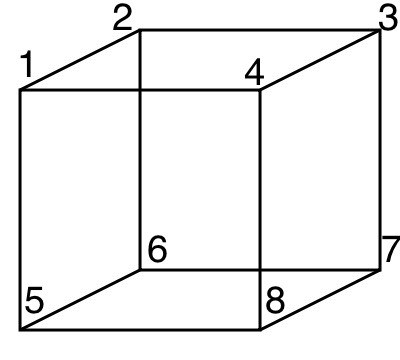
\includegraphics[width=50mm]{Images/cube-ex}\]
Let $G$ be the group of (not necessarily orientation preserving) symmetries of the square. Then $G$ acts on $X$ by permutation of vertices. It's straightforward to see that this $G$ action is transitive, since, e.g. vertex $1$ can be sent to any of the 7 other vertices. Therefore, $|\mathcal{O}_1|=8$ and so $[G:\Stab_G(1)]=8$. That is to say \[|G|=8\cdot |\Stab_G(1)|\] The key is that now we can apply the orbit stabilizer theorem to the restricted $\Stab_G(1)$ action on $X$\footnote{See prop. \ref{restricted-action}}. Let's write $G_1=\Stab_G(1)$. So,  $[G_1 : \Stab_{G_1} (2)]=\mathcal{O}^{G_1}_2$ (we write $\mathcal{O}_1^{G_1}$ here to denote the orbit of $2$ under the action by $G_1$ rather than $G$). When $1$ is fixed, the element $2$ can only be sent to an adjacent vertex to 1. There are three such vertices $2,4$ and $5$, so $|\mathcal{O}_2^{G_1}|=3$. Therefore, \[ |G_1|=3\cdot |\Stab_{G_1}(2)|\] Continuing in this process, let's write $G_2$ for $\Stab_{G_1}(2)$, we can then look at the orbit $\mathcal{O}_3^{G_2}$ of vertex 3 under the action by $G_2$. Since $G_2$ fixes both vertices 1 and 2, 3 must be sent to either itself or 3, that is to say $|\mathcal{O}_3^{G_2}|=2$. Therefore, $[G_2 : \Stab_{G_2}(3)|=2$, and so \[|G_2|=2\cdot |\Stab_{G_2}(3)|\] At this point, if we let $G_3=\Stab_{G_2}(3)$ note that any stabilizers of the $G_3$ action are trivial as a rotation of the cube which fixes vertices $1,2$ and $3$ must be the identity. Therefore, \[ |G|=8\cdot|G_1|\cdot|G_2|=8\cdot 3\cdot 2=48\] 
\end{example}

\begin{remark}
You may recall from example \ref{platonic-solids-ex} that the group of 3D-rotational symmetries of the cube is $S_4$. Note that $|S_4|=24$, not 48 as the previous example shows. What's going on here is that these 3D-rotations must preserve the orientation on 3D space. In example \ref{sym-of-cube-ex}, we calculated the total group of symmetries. Half of these preserve the orientation of the cube, and half don't. 

In fact, we can see exactly what goes wrong. In the last step, we found that $\mathcal{O}_3^{G_2}$ has two elements: 3 and 6. But, if we fix vertices 1 and 2, and swap 3 and 6, the orientation of the cube has been flipped (meaning, this permutation of vertices is not a rotation but a reflection). The previous calculations all preserve orientation, so, if we were tasked with computing the order of the rotational symmetry group of the cube, it would be $8\cdot3=24$ as expected. 

In fact, the group of all symmetries of the cube is isomorphic to $S_4\oplus \mathbf{Z}_2$\footnote{The order checks out, but this shouldn't be ``obvious''. For instance, when talking about dihedral groups $D_n$ is not isomorphic to $\mathbf{Z}_n\oplus \mathbf{Z}_2$, which would be the analog of ``rotational symmetries summed with orientation flip''}.

\end{remark}


\begin{thm}[Burnside's counting lemma] \label{BS-lem} Let $G$ be a finite group and $X$ a finite set with a $G$ action. Let $k=|X/G|$ be the number of orbits of the given $G$ action. Then \begin{equation} 
	k = \dfrac{1}{|G|} \sum_{g\in G} |X^g|
\end{equation}
\end{thm}

In plain English, the term on the right is just the average number of fixed points from the group action. Theorem \ref{BS-lem} can be useful for counting the number of orbits of an action, it's generally easier to intuit fixed points than orbits. 

\begin{proof}[Proof of theorem \ref{BS-lem}]
	This proof employs one of the best combinatorial methods: counting the same thing both ways. Note that \[ \sum_{g\in G} |X^g|= \left|\{ (g,x)\in G\times X : g.x=x\} \right|= \sum_{x\in X} |\Stab_G(x)|\] (Think of laying the points in $G\times X$ out in a grid and counting along the $X$-axes and the $G$-axes respectively in the middle set.)
	
	From theorem \ref{orb-stab} we know that $[G: \Stab_G(x)]=|\mathcal{O}_x|$ and so $|\Stab_G(x)|=|G|/ |\mathcal{O}_x|$. Therefore,\[ \sum_{g\in G} |X^g|= \sum_{x\in X} |\Stab_G(x)|=\sum_{x\in X}\dfrac{|G|}{|\mathcal{O}_x|}=\sum_{Y\in X/G} \left(\sum_{y\in Y} \dfrac{|G|}{|Y|}\right)=\sum_{Y\in X/G}|G|=|G|\cdot|X/G|\]
	(The third equation follows from the observation that orbits partition $X$, so a sum over $X$ can be broken into two sums: an outer sum over all orbits and inner over each element of the orbit). And thus we have that \[ |X/G|=\dfrac{1}{|G|} \sum_{g\in G} |X^g|\]
\end{proof}


\begin{example}[Counting the colors of a square]
	(This is the same example from Judson's book, but his formatting of the answer is difficult to read in my opinion.) Suppose we want to answer the following question: 
	
	\begin{quote} \textit{The vertices of a square are colored either red or green. Up to rotations and reflections, how many such colorings are there?}\end{quote}
	
	Note that the answer is not $2^4=16$, since for instance this number counts each of the labellings of ``all red'' and ``all green'' four times each. We can answer this question using theorem \ref{BS-lem}. Let's first put into language that group actions can handle. 
	
	Let $X=\{1,2,3,4\}$ be the vertices of a square (labeled cyclically). A \textit{coloring} of the square is just a function $c\colon X\to \{ \text{red}, \text{green}\}$. Let's let $C$ denote the set of all such colorings, i.e. \[ C=\left\{ f\colon X\to \{\text{red}, \text{green}\}\right\}\] Note that $D_4$ acts on $C$ as follows: first identify $D_4$ with subgroup\footnote{Here, $r=(1234), s=(12)(34)$} \[D_4'=\{\Id, (1234), (13)(24), (1432), (14)(23), (12)(34), (13), (24)\}\leq S_4\] Then, there is a group action $D_4'\times C\to C$ given by $(\alpha, f)\mapsto f\alpha$, that is, $D_4'$ acts on $C$ by \textit{precomposition} with a permutation \[ X\xrightarrow{\;\alpha\;} X\xrightarrow{\;f\;} \{ \text{red}, \text{green}\}\] Then, a coloring \textit{up to rotation and reflection} is just an \textit{orbit} of this action. Burnside's lemma allows us to calculate the number of orbits by calculating the number of fixed points for each $\alpha\in D_4'$. We have:
	\begin{itemize}
		\item $|C^{\Id}|=16$ --- Any coloring of the square is fixed by the identity permutation.
		\item $|C^{(1234)}|=|C^{(1432)}|=2$ --- Only the colorings of ``all red'' or ``all green'' are fixed by a rotation
		\item $|C^{(12)(34)}|=|C^{(13)(24)}|=|C^{(14)(23)}|=4$ --- Put the vertices into groups of two and color each group the same, there are 4 total such colorings
		\item $|C^{(13)}|=|C^{(24)}|=8$ --- Diagonally opposite vertices get the same color, the other two are colored independently.
	\end{itemize}
	Therefore, the total number of orbits, $k$, is given by \[ k=\dfrac{1}{8}(16+2\cdot2+3\cdot4+2\cdot8)=6\] and thus there are six such distinct colorings of the square. 
\end{example}


\subsection{Exercises}
\begin{enumerate}[label=\arabic*.]
	\item Let $X=\{1,2,3,4,5,6\}$ and $G=\{ \Id, (12), (345), (354), (12)(345), (12)(354)\}\leq S_6$. For each $g\in G$ compute the fixed points $X^g$. For each $x\in X$ compute the stabilizer subgroup $\Stab_G(x)$.
	\item Determine the conjugacy classes for $D_5, \mathbf{Z}_9$ and $Q_8$\footnote{Recall that $Q_8$ is the \textbf{quaternion group} given by $\langle i,j,k | i^2=j^2=k^2=ijk, i^4=j^4=k^4=e\rangle$}
	\item Let $A_4$ act on $S_4$ by conjugation, i.e., $\beta.\alpha=\beta \alpha \beta^{-1}$ for $\alpha\in S_4, \beta\in A_4$. Describe the orbits of this action. 
	\item Let $X=\{1,2,3,\dots,n\}$ and let $S_n$ act on $X$ by permutation. Is this action transitive? Is the action by the alternating group $A_n$ on $X$ transitive? 
	\item Let $X=\{(u,v): u,v\in \mathbf{R}^2 \text{ are linearly independent vectors}\}$ and $\GL_2(\mathbf{R})$ act on $X$ by $A.(u,v)=(Au,Av)$. Is this action transitive? 
	\item Let $\SL_2(\mathbf{R})$ act on $\mathbf{R}^2$ by $A.v=Av$. Is this action transitive? 
%item Let $\SO(2)$ denote the group of matrices \[ \SO(2)=\left\{\begin{pmatrix} \cos\theta & -\sin \theta \\ \sin \theta & \cos \theta\end{pmatrix} : \theta \in \mathbf{R}/2\mathbf{Z}\right\}\] 
	\item Let $X$ be a set with an action of a group $G$. Prove the following:
	\begin{enumerate}
		\item $\bigcap_{g\in G}X^g=X^G$
	\end{enumerate}
	\item Use the proof technique from example \ref{sym-of-cube-ex} to compute the order of the symmetry groups for the tetrahedron, octahedron, icosahedron, and dodecahedron (see also, example \ref{platonic-solids-ex})
	\item Up to 3D rotations how many distinct enumerations of a six-sided die are there? What about a four-sided die?
	\item Up to rotations and reflections, how many ways can the vertices of a hexagon be colored red or green?
	\item A cube consists of 12 edges. Suppose these edges are colored yellow and green. Up to 3D rotations, how many such colorings of the cube are there?
	\item \href{https://en.wikipedia.org/wiki/Benzene}{Benzene} is an organic compound made of a ring of six carbon atoms $C$ attached to hydrogen atoms $H$ as below:
	\[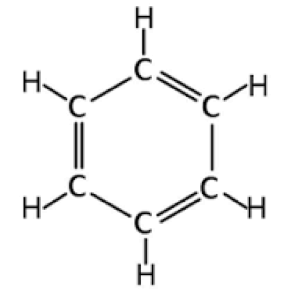
\includegraphics[width=40mm]{Images/benzene-ex}\]
	
	Suppose one or more hydrogen atoms is replaced with chlorine. How much different compounds can be made? What if three of the six $H$ atoms were replaced by a single $CH_3$.
	
	\item Suppose that $G$ acts on a set $X$. This action is called \textbf{faithful} if given $g\in G$ such that $g.x=g.y$ then $x=y$ (i.e., the functions $\varphi_g\colon X\to X$ are injective) Similarly the action is called \textbf{full} if given $y\in X$ there is $x\in X$ with $g.x=y$ (i.e., $\varphi_g$ are surjective). Determine if the following actions are faithful and/or full:
	\begin{enumerate}
		\item $S_3$ acting on $\{1,2,3\}$
		\item $V=\{\Id, (13), (24), (13)(24)\}$ on $\{1,2,3,4\}$
		\item $\GL_2(\mathbf{R})$ acting on $\mathbf{R}^2$ by $A.v=Av$
		\item $\mathbf{Z}_5$ acting on a regular pentagon by rotation on the vertices.	
		\item $\mathbf{Z}_4$ acting on the cube by rotation  through one central axis of the cube
	\end{enumerate}
	
	\item Let $G$ be the symmetry group of the \textit{hypercube} (i.e., 4-dimensional cube, see picture below). Let $X=\{1,2,3,4,\cdots, 15,16\}$ be the set of vertices of the hypercube, and let $G$ act on $X$ by permutation of vertices. Use a similar argument to example \ref{sym-of-cube-ex} to determine the order of $G$. 
	\[ 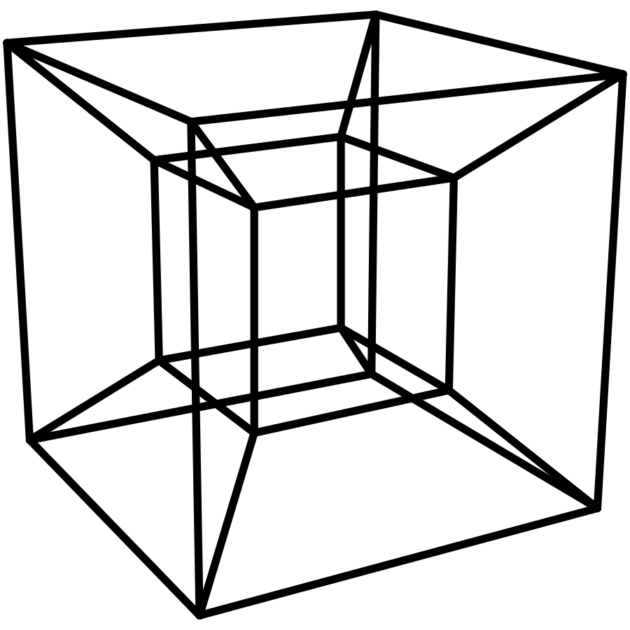
\includegraphics[width=50mm]{Images/hypercube-ex1}\] 
\end{enumerate}

\section{Matrix groups} 

Historically, all groups were subgroups of symmetric groups. A (slightly) more modern approach is to think of groups in how they can be ``put'' inside groups of matrices\footnote{This is essentially the field of \href{https://en.wikipedia.org/wiki/Representation_theory}{representation theory}}. Our focus will be on matrices will real coefficients, but there is an equally deep story for the following content when $\mathbf{R}$ is replaced by $\mathbf{C}$, the complex numbers, or more generally some arbitrary field (for instance, matrices with coefficients in $\mathbf{Z}_p$ are another big topic to explore). 

Recall that definitions we've been working with so far \begin{equation} \GL_n(\mathbf{R}) = \{A : \text{$A$ is an $n\times n$ invertible matrix with real entires}\}\end{equation} and 
\begin{equation} \SL_n(\mathbf{R}) = \{A\in \GL_n(\mathbf{R}) : \det A=1\}\end{equation}

In words, we call these the \textbf{general linear} group and \textbf{special linear} group of $n\times n$ matrices (with real coefficients), respectively. We've already seen that $\SL_n (\mathbf{R})\nrml \GL_n(\mathbf{R})$, since $\SL_n(\mathbf{R})$ is the kernel of the determinant $\det \colon \GL_n (\mathbf{R})\to\SL_n(\mathbf{R})$. 




Let's denote by $I\in \GL_n(\mathbf{R})$ the identity matrix (i.e., $I$ has 1s along the diagonal and 0s everywhere else). Matrices can be given by double indexed sets, i.e., $A=\{a_{i,j}\}_{1\leq i,j\leq n}$ where the entries $a_{i,j}$ for $i=1,\dots n$ are the entries over the $j$-th column, and $a_{i,j}$ for $j=1,\dots,n$ are the entries from the $i$-th row of $A$

\begin{defn}[Matrix transpose] Let $A=\{a_{i,j}\}\in \GL_n(\mathbf{R})$. Then the \textbf{transpose of $A$} is the matrix $A^T$ given by $A^T=\{a_{j,i}\}$
\end{defn}



Visually, the transpose of a matrix is just the reflection of the entries of $A$ over the main diagonal. I leave you to check the following proposition. More generally, matrix transposition is an instance of $\mathbf{Z}_2$ acting on $\GL_2(\mathbf{R})$, which I also leave you to check. 

\begin{prop} \label{transposition-ex}
	For matrices $A,B\in \GL_n(\mathbf{R})$, we have $(AB)^T=B^TA^T$ and $(A^{-1})^T=(A^T)^{-1}$.
\end{prop}


\begin{defn}[Symmetric matrix]
Let $A$ be an $n\times n$ matrix. Then $A$ is \textbf{symmetric} if $A=A^T$. 
\end{defn}
\subsection{Orthogonal matrices}

\begin{defn}[Orthogonal matrix] An $n\times n$ matrix with real entries is called \textbf{orthogonal} if $A^TA=I$. 
\end{defn}

\begin{example}\label{orthogonal}
Let's unpack what this definition is telling us: Suppose we are given a matrix $A\in \GL_3(\mathbf{R})$ of the form \[A=\begin{pmatrix} a_{1,1} & a_{1,2} & a_{1,3} \\ a_{2,1} & a_{2,2} & a_{2,3} \\ a_{3,1} & a_{3,2} & a_{3,3} \end{pmatrix}\]
Then: 
 \[A^T=\begin{pmatrix} a_{1,1} & a_{2,1} & a_{3,1} \\ a_{1,2} & a_{2,2} & a_{3,2} \\ a_{1,3} & a_{2,3} & a_{3,3} \end{pmatrix}\]

Let's write out the product $A^TA$ (it's going to be long)
\begin{equation*} \label{Ex-A-orth}A^TA=
\begin{pmatrix} (a_{1,1})^2+(a_{2,1})^2+(a_{3,1})^2 & 
a_{1,1}a_{1,2} + a_{2,1}a_{2,2} + a_{3,1}a_{3,2} &
 a_{1,1}a_{1,3}+a_{2,1}a_{2,3}+a_{3,1}a_{3,3} \\
 a_{1,2}a_{1,1} +a_{2,2}a_{2,1}+a_{3,2}a_{3,1}& 
  (a_{1,2})^2+(a_{2,2})^2+(a_{2,3})^2 & 
  a_{1,2}a_{2,3}+a_{2,2}a_{2,3}+a_{3,2}a_{3,3} \\ 
  a_{1,3}a_{1,1}+a_{2,3}a_{2,1} + a_{3,3}a_{3,1} &
  a_{1,3}a_{1,2}+a_{2,3}a_{2,2}+a_{3,3}a_{3,2} & 
   (a_{1,3})^2+(a_{2,3})^2+(a_{3,3})^2\end{pmatrix}
\end{equation*}

This looks like a nightmare but something nice is happening. Let's suppose that $A$ is orthogonal. Recall then that this means that $A^TA$ from the equation above is then equal to the identity matrix \[I=\begin{pmatrix} 1 & 0 & 0\\ 0 & 1 & 0 \\ 0 & 0 & 1\end{pmatrix}\]
Let's let $v_1=(a_{1,1}, a_{2,1}, a_{3,1})$, $v_2=(a_{2,1}, a_{2,2}, a_{2,3})$ and $v_3=(a_{1,3}, a_{2,3}, a_{3,3})$ be vectors in $\mathbf{R}^3$. And note that the dot products $v_i\cdot v_j$ are precisely the entries of $A^TA$: \[ A^TA=\begin{pmatrix} v_1\cdot v_1 & v_1\cdot v_2 & v_1\cdot v_3 \\ v_2\cdot v_1 & v_2\cdot v_2 & v_3 \cdot v_2 \\ v_3 \cdot v_1 & v_3\cdot v_2  & v_3\cdot v_3\end{pmatrix}\]  That is to say, if $A$ is orthogonal, then the column vectors (in this case $v_1,v_2,v_3$) from $A$ satisfy the following: \[ v_1\cdot v_1=1,\, v_2\cdot v_2=1, \,v_3\cdot v_3=1; \quad v_i\cdot v_j=0 \text{ (for $i\neq j$) }\]
In other words still, the columns of $A$ form an \textbf{orthonormal basis}\footnote{i.e., a basis such that each basis element is of unit length and any two distinct elements of the basis are orthogonal} of $\mathbf{R}^3$.
\end{example}

\begin{defn} 
Let $n\geq 1$. Define $\Or(n)$ to be the set of orthogonal matrices $A\in \GL_n(\mathbf{R})$. Similarly define $\SO(n)\subset \Or(n)$ to be the collection of orthogonal matrices $A$ such that $\det A=1$. 
\end{defn}

In words, $\Or(n)$ is called the \textbf{orthogonal group} (of order $n$) and $\SO(n)$ the \textbf{special orthogonal group} (also of order $n$). That these sets actually form subgroups of $\GL_n(\mathbf{R})$ follows from prop \ref{On-group}. From example \ref{orthogonal} we know that any matrix $A\in \Or(n)$ is represented by some orthonormal basis of $\mathbf{R}^n$. If furthermore $A\in \SO(n)$ then $A$ is \textit{orientation preserving}: that is, the standard orientation\footnote{For instance, in $\mathbf{R}^3$ this is the \textit{right-hand rule}} on the basis of coordinate axis in $\mathbf{R}^n$ is preserved under $A$.

\begin{prop}\label{On-group}
	Let $n\geq 1$ then $\Or(n)$ and $\SO(n)$ are groups. Moreover, \[\SO(n)\nrml O(n)\leq \GL_n(\mathbf{R})\]
\end{prop}

\begin{prop} $\Or(2)$ and $\SO(2)$ are given by the following:	\begin{itemize}
	\item $\Or(2)=\left\{ \pm \begin{pmatrix} \cos\theta & -\sin\theta \\ \sin\theta & \cos\theta \end{pmatrix} : \theta \in \mathbf{R}\right\}$
	
	\item $\SO(2)=\left\{ \begin{pmatrix} \cos\theta & -\sin\theta \\ \sin\theta & \cos\theta \end{pmatrix} : \theta \in \mathbf{R}\right\}$
	\end{itemize}
\end{prop}

\begin{corollary}
	$\SO(2)\cong \mathbf{R}/2\pi\mathbf{Z}$
\end{corollary}

\subsection{Rotations of real space}
When you think of a rotation of space, what really is happening is an orientation preserving change of orthonormal basis for $\mathbf{R}^n$. That is to say, the group $\SO(n)$ captures the rotational structure of $\mathbf{R}^n$. 

For instance, the following propositions tells us what \textit{finite rotational symmetries} look like in $\mathbf{R}^2$ and $\mathbf{R}^3$. 


\begin{prop}
	Let $H\leq \SO(2)$ be a finite subgroup. Then $H$ is isomorphic to $\mathbf{Z}_n$ for some $n\geq 1$.
\end{prop}

In particular $H$ is generated by a matrix of the form \[ R=\begin{pmatrix} \cos(2\pi/n) & -\sin(2\pi/n) \\ \sin(2\pi/n) & \cos(2\pi/n) \end{pmatrix} \]

\begin{prop}
	Let $H\leq \SO(3)$ be a finite subgroup. Then $H$ is isomorphic to one of the following groups \begin{itemize}
		\item $\mathbf{Z}_n$ (for some $n\geq 1$)
		\item $D_n$ (for some $n\geq 1$)
		\item $A_4, \, S_4$ or $A_5$
	\end{itemize}
\end{prop}

In particular, these symmetries can be realized as group actions as follows: \begin{itemize}
	\item $\mathbf{Z}_n$ acts on a (thickened) $n$-gon in $\mathbf{R}^3$ by rotation 
	\item $D_n$ acts on a (thickened) $n$-gon in $\mathbf{R}^3$ by rotations and reflections
	\item $A_4$ acts on the tetrahedron as orientation preserving symmetries
	\item $S_4$ acts on the cube and octahedron as orientation preserving symmetries
	\item $A_5$ acts on the icosahedron and dodecahedron as orientation preserving symmetries
\end{itemize}

A precise proof is a bit beyond the scope of our class. But, here's a heuristic argument: if $H\leq \SO(3)$ were some finite subgroup not from this list, then $H$ would be the rotational symmetry of some shape. If this were a 3D shape it would have be a (finite) regular polyhedron. But, we've already enumerated all of the regular polyhedra (the Platonic solids) and their symmetry groups. 

\begin{remark} A question I get a lot from students is ``What is the fourth dimension". The (cheap) but ``correct'' answer of the ``fourth dimension is just $\mathbf{R}^3$ with another axis" does not really satisfy. What you really want is to understand the structure of $\SO(4)$: Our intuition about 3-dimensional space is built off of interacting (i.e., rotating) actual 3D objects all our life, we implicitly understand the group structure of $\SO(3)$ even if we don't know it by name. 

Meaning, if you want to get a better understanding of 4D space, you can start by understanding what $\SO(4)$ looks like: What kind of subgroups does it have? For instance, the quaternion group $Q_8$ is (isomorphic to) a \href{https://groupprops.subwiki.org/wiki/Linear_representation_theory_of_quaternion_group#Four-dimensional_irreducible_representation_over_a_non-splitting_field}{subgroup} of $\SO(4)$ (and notably $Q_8$ is not a subgroup of $\SO(3)$), so is a ``new'' type of rotational symmetry unlocked with the additional dimension.  What's nice, is that with some understanding of matrix operations, and our newly acquired language of group theory, we can begin to understand how to answer this question (and the same questions for higher dimensional spaces still). 

Another thing to point out is that these matrix groups are \textit{manifolds} (essentially, ``shapes" that have geometry). Meaning, you can talk about \textit{paths of rotations} as just parametrized curves in the space $\SO(n)$. Even in $\mathbf{R}^3$ some bizarre things\footnote{For instance, the \href{https://en.wikipedia.org/wiki/Plate_trick}{Plate trick}} happen that are not immediately obvious, but give us deep insight to the geometry of space (and also show up when, e.g., describing certain types of symmetries in particle physics) 
\end{remark}


\subsection{Exercises}
\begin{enumerate}[label=\arabic*.]

	\item Prove proposition \ref{transposition-ex}. Then prove that $A\mapsto A^T$ describes an action by $\mathbf{Z}_2$ on $\GL_n(\mathbf{R})$. 
	\item Let $E(n)=\{ (A,x) : A\in \Or(n), x\in \mathbf{R}^n\}$. Define a binary operation on $E(n)$ by \[(A,x)\cdot (B,y)=(AB,Ay+x)\] Prove that $E(n)$ is a group.
	
	\item \label{rotations-R3} Let $\theta\in\mathbf{R}$. Prove that the following matrices are all elements of $\SO(3)$ \[ R_x(\theta)=\begin{pmatrix} 1 & 0 & 0 \\ 0 & \cos\theta & -\sin\theta \\ 0 & \sin\theta & \cos\theta \end{pmatrix} \quad 
	R_y(\theta)=\begin{pmatrix} \cos\theta & 0 &  \sin\theta \\ 0 &1 & 0 \\-\sin\theta & 0 & \cos\theta \end{pmatrix} \quad 
	R_z(\theta)=\begin{pmatrix}  \cos\theta & -\sin\theta& 0 \\ \sin\theta & \cos\theta & 0 \\ 0 & 0 & 1\end{pmatrix}\]
	and then prove that $R_x(\theta),R_y(\theta),R_z(\theta)$ denote (counterclockwise) rotations by $\theta$ of the $x$-, $y$- and $z$-axes in $\mathbf{R}^3$. 
	
	\item Let $\theta,\psi$ be real numbers. Prove that $\SO(4)$ contains the following matrix \[ R_{\theta,\psi} = \begin{pmatrix} \cos \theta & - \sin\theta & 0 & 0 \\
\sin\theta & \cos\theta & 0 & 0 \\
0 & 0 & \cos\psi & -\sin\psi \\
0 & 0 & \sin\psi & \cos\psi\end{pmatrix}\]
Use this show that $\SO(2)\oplus \SO(2)\leq \SO(4)$. Is there an $n$ such that $\Or(2)\oplus \Or(2)\leq \SO(n)$?

Follow up: Does $\SO(4)$ contain the following matrix?  \[\widetilde{R_{\theta,\psi}} = \begin{pmatrix} 0 & 0 & \cos \theta & - \sin\theta  \\
0 & 0 &\sin\theta & \cos\theta  \\
\cos\psi & -\sin\psi & 0 & 0\\
 \sin\psi & \cos\psi & 0 & 0 \end{pmatrix}\]
	
	\item Let $\Delta_n$ be a regular $n$-gon centered at the origin in $\mathbf{R}^2$ and let $\Or(2)$ act on $\mathbf{R}^2$ by $(A,x)\mapsto Ax$. Prove that $\Stab_{\Or(2)}(\Delta_n)\cong D_n$ the $n$-th dihedral group.
	
	\item Let $\SO(3)$ act on $\mathbf{R}^3$ by $(A,x)\mapsto Ax$. Is this action transitive? Determine the set of orbits from this action. 

	\item Let $A\in \GL_n(\mathbf{R})$ be a symmetric matrix. Prove that the eigenvalues of $A$ are always real numbers and that any two nonparallel eigenvectors of $A$ are perpendicular. 
	
	\item \label{bilinear-form}Let $A$ be a symmetric $n\times n$ matrix, i.e., a matrix such that $A^T=A$ and $x,y\in \mathbf{R}^n$ be column vectors. Let $\langle x,y\rangle_A$ be given by \[\langle x,y\rangle_A=x^T A y\]
	Prove that the following hold: \begin{enumerate}
		\item $\langle x, y\rangle_A=\langle y,x\rangle_A$
		\item $\langle x, y+z\rangle_A=\langle x, y\rangle_A+\langle x, z\rangle_A$
		\item $\langle kx, y\rangle_A=k\langle x, y\rangle_A$ \quad for any scalar $k$
		%\item $\langle x,x\rangle_A\geq 0$
		%\item If $\langle x,y\rangle_A=0$ for all $y\in \mathbf{R}^n$ then $y=0$.
	\end{enumerate}
	Such an operation $(x,y)\mapsto \langle x,y\rangle_A$ is called an \textit{bilinear form}. Prove further that if $A=\Id$ then $\langle x,y\rangle_{\Id}=x\cdot y$ the \textit{dot product} of vectors $x,y$.

	

	\item True or False: There is an $n\geq 1$ such that  $\Or(n)$ has an abelian subgroup of infinite cardinality. 
	\item Let $n\leq m$. Show that $\Or(n)\leq \Or(m)$ and $\SO(n)\leq \SO(m)$.
	\item Let $n\geq 1$. Prove that $S_n\leq \Or(n)$. Is it also the case that $S_n\leq \SO(n)$?
	
	\item \textit{Challenge}. (Follow up to problem \ref{rotations-R3}). Let $v$ be some vector in $\mathbf{R}^3$ and $\theta\in \mathbf{R}$. Write  $R_v(\theta)$ for the element in $\SO(3)$ given by rotation about the axis produced by $v$ in the counterclockwise direction. Denote by $L_v$ the following matrix \[ L_v = \dfrac{d}{d\theta} \left[R_v(\theta) \right]_{\theta=0}\]
	Note that $L_v$ is the \textit{instantaneous rotation} through axis $v$ when $\theta=0$. 
	Let ${x}=(1,0,0), {y}=(0,1,0), {z}=(0,0,1)$ denote the vectors in the positive $x$-, $y$-, and $z$-axes respectively.
	\begin{enumerate}
	\item Prove that for any (column) vector $u$, $L_v u =v\times u$. 
	\item Prove that \[ L_x= \begin{pmatrix} 0 & 0 & 0 \\ 0 & 0 & -1 \\ 0 & 1 & 0\end{pmatrix} \quad L_y=\begin{pmatrix} 0 & 0 & 1 \\ 0 & 0 & 0 \\ -1 & 0 & 0 \end{pmatrix} \quad L_z=\begin{pmatrix} 0 & -1 & 0 \\ 1 & 0 & 0 \\ 0 & 0 & 0 \end{pmatrix}\]
	\item Prove that $L_x L_y-L_yL_x=L_z$, $L_yL_z-L_zL_y=L_x$ and $L_zL_x-L_xL_z=L_y$
	\item For a vector $v=(a,b,c)$, show that $L_v$ is given by  \[L_v=aL_x+bL_y+cL_z.\]
	\item Prove that for vectors $u,v$, the cross product $u\times v$ satisfies \[ L_{u\times v}=L_uL_v-L_uL_v.\]
	
	The (real) vector space with basis $L_x,L_y,L_z$ is (an isomorphic form) of the associated \textit{Lie algebra} to the \textit{Lie group} $\SO(3)$. It's usually written $\mathfrak{so}(3)$. Though this may look intimidating (and it is), what you've just shown is that $\mathfrak{so}(3)$ is isomorphic (as algebras) to $\mathbf{R}^3$ equipped with the cross-product.
	\end{enumerate}
	
	\item \textit{Challenge}. (Follow up to problem \ref{bilinear-form}). You may recall the \textit{second-derivative test}\footnote{That is, if $(a,b)$ is a point such that $\nabla f(a,b)=0$ then the Hessian determinant $D=f_{xx}f_{yy}-f_{xy}^2$ evaluated at $(a,b)$ can be used to determine if $(a,b)$ is a max/min or saddle point.} from multivariable calc. If $f\colon \mathbf{R}^3\to\mathbf{R}$ is a differentiable function of three variables, write $H$ for the Hessian matrix \[ H= \begin{pmatrix} f_{xx} & f_{xy} & f_{xz} \\ f_{yx} & f_{yy} & f_{yz} \\ f_{zx} & f_{zy} & f_{zz} \end{pmatrix}\]Here, $f_{xy}$ denotes the partial derivative $\partial^2 f/\partial x\partial y$, etc. Note $H$ is a function of the variables $x,y,z$.
	\begin{enumerate}
		\item Prove that $H$ is symmetric
		\item Prove that for a column vector $v\in\mathbf{R}^3$, that $\langle v,v\rangle_H$ is equal to the concavity of $f$ in the direction $v$.
		\item Prove that if (at a point $P\in\mathbf{R}^3$ such that $\nabla f(P)$ is the zero vector) that if all eigenvalues of $H$ are positive, then $P$ is a local minimum of $f$. 
	\end{enumerate}	

	

\end{enumerate}

\appendix
\section{Mathematical induction}

Induction, or \textbf{mathematical induction}, is a useful tool for proving (or in many cases ``confirming'') the existence of some pattern, usually dependent on the natural numbers. Rather than give a general description of what induction is, it's better to look at the following example and see how to use induction. 

\begin{example} A classic example is proving the sum formula \begin{equation} 1+2+3+\cdot+n=\dfrac{n(n+1)}{2} \label{sum1} \end{equation} holds for all $n\geq 1$. It goes as follows: let's first show that the formula holds for $n=1$. Since \[ 1 = \dfrac{1(1+1)}{2}=\dfrac{2}{2}=1\] this is indeed true. Here's the trick: we show that \textit{if} the formula is true for some value of $n$, then it \textit{must} be true for $n+1$ as well. Let's see \begin{align*}
1+2+\cdots+n+(n+1) &= \dfrac{n(n+1)}{2}+n+1\\ &= \dfrac{ n(n+1)+2(n+1)}{2}\\&= \dfrac{(n+1)(n+2)}{2}\end{align*}
So, by induction, \eqref{sum1} must hold for all $n$.
\end{example}

It's important to note what we've just shown. Let's let $P(n)$ be the statement that the formula \eqref{sum1} holds for $n$. In the first step we showed $P(1)$ is true. Then we showed that $P(n)$ implies $P(n+1)$. At this point it's like watching a bunch of dominoes topple over. We get that $P(1)$ is true, so $P(2)$ must be. But then $P(3)$ must be, and $P(4)$, and $P(5)$,  and so on. If we give ourselves an arbitrary $n$ and ask the question ``is $P(n)$ true?'' the answer must be ``yes'' as we can work our way back to its truth value being tied to $P(1)$, which was already shown. Note as well that induction doesn't tell us ``what'' the formula \eqref{sum1} should be. It only allows us to prove that the formula is correct. 


\subsection{Using induction}

Induction is typically used to prove statements like \eqref{sum1} which can be phrased as a set of propositions $\{P(n) : n\in \mathbf{N}\}$ which have a decent ``regularity'' to them. A general approach to using induction is then:
\begin{itemize}
	\item Show that there is a ``starting value'' $k\in\mathbf{N}$ such that $P(k)$ is true. Typically this is $k=1$, but it doesn't have to be. This is called the \textbf{base case}.
	\item Show that given an arbitrary $n\geq k$, that if $P(n)$ is true, then $P(n+1)$ must be true. This is called the \textbf{inductive step}.
\end{itemize}
A good proof by induction will then end by justifying why and how induction has been used, but the above steps are where the work goes in. 

\subsection{Well-orderings}
What induction relies on is that the set $\mathbf{N}$ is well-ordered\footnote{And in fact this is a sufficient condition \textit{do} induction, meaning you can ``do induction'' over any well-ordered set, even those with uncountably many elements, it's just harder to intuit what is happening}. A complete definition is given below for your entertainment, but we won't really need to go any deeper into well-orderings than understanding how to use theorem \ref{well-ord}. 

\begin{defn}Let $X$ be a set. An \textbf{ordering} on $X$ is a relation $\leq$ on $X$ such that~\begin{itemize}
\item For each pair of elements $x,y\in X$ either $x\leq y$ or $y\leq x$
\item $x\leq x$ for all $x\in X$
\item If $x,y,z\in X$ such that $x\leq y$ and $y\leq z$, then $x\leq z$.
\item If $x\leq y$ and $y\leq x$, then $x=y$. 
\end{itemize}
\end{defn}
 
A set $X$ with ordering $\leq$ is called \textbf{well-ordered} if each nonempty subset $Y\subset X$ has a least-element for this ordering (that is, there is $y\in Y$ such that $y\leq z$ for all $z\in Y$). You can convince yourself that $\mathbf{N}$ is well-ordered, but $\mathbf{Z}$ is not (at least with the typical ordering of integers). A fun, \href{https://en.wikipedia.org/wiki/Constructivism_(philosophy_of_mathematics)}{but somewhat controversial}, fact in mathematics is that \textit{any} set can be well-ordered. 

For us, it's enough to use the following as a black-box statement (which is true more or less by definition). 

\begin{thm}[$\mathbf{N}$ is well-ordered]\label{well-ord}
	Any nonempty subset $X\subset \mathbf{N}$ has a smallest element. 

\end{thm}

\subsection{Exercises} 
\begin{enumerate}[label=\arabic*.]
	\item Use induction to prove for $n\geq 1$ that \[ 1^2+2^2+3^3+\cdots+n^2=\dfrac{n(n+1)(2n+1)}{6}\] 
	\item Use induction to prove that $n!>2^n$ for $n\geq 4$. 
	\item Use induction to prove for $n\geq 2$ that \[ \dfrac{1}{1\cdot 2} + \dfrac{1}{2\cdot 3} + \dfrac{1}{3\cdot 4} +\cdots + \dfrac{1}{(n-1)n} = \dfrac{n-1}{n}\]
	\item You may know about the Fibonacci numbers: $a_1=1, a_2=1$ and $a_{n}=a_{n-1}+a_{n-2}$ for $n\geq 3$. Prove for $n\geq 1$ that \[ a_n=\dfrac{1}{\sqrt{5}}  \left( \dfrac{1+\sqrt{5}}{2} \right)^n- \dfrac{1}{\sqrt{5}}\left(\dfrac{1-\sqrt{5}}{2}\right)^n\]  
	
	\textit{Challenge}. What is the limit $\lim_{n\to \infty} a_{n+1}/a_n$ of the ratio of successive Fibonacci numbers?
	\item With respect to the usual ordering, are the sets $\mathbf{Q}$ or $\mathbf{R}$ well-ordered?
	
	\item Prove that for any $n\geq 1$ there is an integer $k$ such that \[ 10^{n+1}+10^{n}-1=3k\] 
	
	\item \textit{Challenge}. Let $n\geq 1$ and let $a_1,a_2,\cdots, a_n$ be real numbers. Prove that \[ \sqrt[n]{a_1a_2a_3\cdots a_n}\leq \dfrac{1}{n} \sum_{k=1}^n a_k\] This is known as the \href{https://en.wikipedia.org/wiki/AM\%E2\%80\%93GM_inequality}{AM-GM inequality}.
	\item \textit{Challenge}. Let $S=\{0,1\}\times \mathbf{N}$ and give $S$ the order that $(a,b)\leq (c,d)$ if either (i)  $a=c, b\leq d$ or (ii)  $a<c$\footnote{This is sometimes called the \textit{lexicographic order}}. Show that $S$ is well-ordered. Show as well that there is no bijection $f\colon S\to \mathbf{N}$ that preserves this ordering $\leq$ (that is, such that if $a\leq b$ in $S$ then $f(a)\leq f(b)$ in $\mathbf{N}$).
\end{enumerate}


\end{document}









	
